\documentclass[12pt,a4paper,twoside]{book}
\usepackage[utf8]{inputenc}
\usepackage{amsmath}
\usepackage{amstext}
\usepackage{amsfonts}
\usepackage{amssymb}
\usepackage{graphicx}
\usepackage{longtable}
\usepackage{booktabs}
\usepackage[bookmarks=true,colorlinks=true,urlcolor=blue,citecolor=blue,linkcolor=blue,unicode=true]{hyperref}
\usepackage[top=2.5cm, bottom=2.5cm]{geometry}
\usepackage{siunitx}

\setlength{\parindent}{0pt}
\setlength{\parskip}{6pt plus 2pt minus 1pt}
\setlength{\emergencystretch}{3em}  % prevent overfull lines
\providecommand{\tightlist}{%
  \setlength{\itemsep}{0pt}\setlength{\parskip}{0pt}}

%predefined commands
\newcommand{\Cb}{C_\beta} 
\newcommand{\eq}{\!=\!} 
\newcommand{\Gauss}{\mathcal{N}} 
\renewcommand{\H}{\mathbf{H}} 
\newcommand{\Hij}{\H_{ij}} 
\newcommand{\I}{\mathbf{I}} 
\newcommand{\Lijk}{\mathbf{\Lambda}_{ij,k}}
\newcommand{\Lk}{\mathbf{\Lambda}_k}
\newcommand{\LLreg}{L\!L_\mathrm{reg}}
\newcommand{\muijk}{\mathbf{\mu}_{ij,k}}
\newcommand{\muk}{\mathbf{\mu}_k}
\newcommand{\neff}{N_\mathrm{eff}}
\renewcommand{\r}{\mathbf{r}}
\newcommand{\rij}{r_{ij}}
\newcommand{\seq}{\mathbf{x}}
\newcommand{\Qij}{\mathbf{Q}_{ij}}
\newcommand{\q}{\mathbf{q}}
\newcommand{\qij}{\mathbf{q\prime}_{ij}}
\newcommand{\Sn}{S_n}
\renewcommand{\v}{\mathbf{v}}
\newcommand{\vi}{v_{i}}
\newcommand{\vj}{v_{j}}
\newcommand{\via}{v_{ia}}
\newcommand{\w}{\mathbf{w}}
\newcommand{\wij}{\mathbf{w}_{ij}}
\newcommand{\wijab}{w_{ijab}}
\newcommand{\wijcd}{w_{ijcd}}
\newcommand{\wklcd}{w_{klcd}}
\newcommand{\X}{\mathbf{X}}
\newcommand{\angstrom}{\mathring{A} \;}


% Numbering of sections unto depth=5
\setcounter{secnumdepth}{5}

% Table of contents formatting
\renewcommand{\contentsname}{Table of Contents}
\setcounter{tocdepth}{1}

% Headers and page numbering 
\usepackage{fancyhdr}
\pagestyle{plain}

% Chapter styling
\usepackage[grey]{quotchap}
\makeatletter 
\renewcommand*{\chapnumfont}{%
  \usefont{T1}{\@defaultcnfont}{b}{n}\fontsize{80}{100}\selectfont% Default: 100/130
  \color{chaptergrey}%
}
\makeatother


%------------------- Definition of LMU title pages
\newcommand{\LMUCover}[3]{
    \thispagestyle{empty}
    {\parindent0cm \rule{\linewidth}{.7ex}}
    
    \begin{flushright}
      \vspace*{\stretch{1}}
      \sffamily\bfseries\Huge
      #1\\
      \vspace*{\stretch{1}}
      \sffamily\bfseries\large
      #2
      \vspace*{\stretch{1}}
    \end{flushright}
  
    \rule{\linewidth}{.7ex}
    \vspace*{\stretch{5}}
    \vspace*{\stretch{1}}
    
    \begin{center}\sffamily\LARGE{#3}\end{center}
}



\newcommand{\LMUTitlePage}[4]{
    \thispagestyle{empty}
    \vspace*{\stretch{1}}
    
    \begin{center}
      \Large Dissertation zur Erlangung des Doktorgrades der Fakultät für Chemie und Pharmazie der Ludwig-Maximilians-Universität München
    \end{center}
    
    \vspace*{\stretch{1}}
    {\parindent0cm \rule{\linewidth}{.7ex}}
    
    \begin{flushright}
      \vspace*{\stretch{1}}
      \sffamily\bfseries\Huge
      #1\\
      \vspace*{\stretch{1}}
    \end{flushright}
  
    \rule{\linewidth}{.7ex}

    \vspace*{\stretch{3}}
    \begin{center}
      \Large vorgelegt von\\
      \Large #2\\
      \Large geboren in #3\\
      \vspace*{\stretch{2}}
      \Large München, den #4
    \end{center}
}


\newcommand{\LMUErklaerung}[5]{
    \thispagestyle{empty}
    \begin{flushleft}
      \large \textbf{Erklärung} \\[1mm]
      \large Diese Dissertation wurde im Sinne von §7 der Promotionsordnung vom 28. November 2011 von #2 betreut.
      \bigskip
  
      \large \textbf{Eidesstattliche Versicherung}\\[1mm]
      \large Diese Dissertation wurde eigenständig und ohne unerlaubte Hilfe erarbeitet.
      \vspace{5em}
  
      \dots\dots\dots   \dots\dots\dots \hfill \dots\dots\dots\dots\dots\dots\dots\dots\\
      \large Ort, Datum \hfill #1
      \vfill
  
  
      \large Dissertation eingereicht am: \hfill #4
      \bigskip
    
      \large Erstgutachter:  #2 \hfill \dots\dots\dots\dots\dots\dots\dots
      \bigskip
    
      \large Zweitgutachter: #3 \hfill \dots\dots\dots\dots\dots\dots\dots
      \bigskip
    
      \large Tag der mündlichen Prüfung: \hfill #5
    \end{flushleft}
}


\usepackage{amsthm}
\newtheorem{theorem}{Theorem}[chapter]
\newtheorem{lemma}{Lemma}[chapter]
\theoremstyle{definition}
\newtheorem{definition}{Definition}[chapter]
\newtheorem{corollary}{Corollary}[chapter]
\newtheorem{proposition}{Proposition}[chapter]
\theoremstyle{definition}
\newtheorem{example}{Example}[chapter]
\theoremstyle{remark}
\newtheorem*{remark}{Remark}
\begin{document}

\frontmatter

%%% LMU cover page
\LMUCover
	{Bayesian Model for Prediction of Protein Residue-Residue Contacts}
	{Susann Vorberg}
	{15.10.2017}

\newpage
\thispagestyle{empty}
\cleardoublepage

%%% LMU title page
\LMUTitlePage
	{Bayesian Model for Prediction of Protein Residue-Residue Contacts}
	{Susann Vorberg}
	{Leipzig, Germany}
	{15.10.2017}

\newpage
\thispagestyle{empty}
\cleardoublepage

%%% LMU statement page
\LMUErklaerung
	{Susann Vorberg}
	{Dr. Johannes Soeding}
	{Prof. Dr. Julien Gagneur}
	{15.10.2017}
	{15.12.2017}

\newpage
\thispagestyle{empty}
\cleardoublepage
\frontmatter\setcounter{page}{1}

\chapter*{Summary}\label{summary}
\addcontentsline{toc}{chapter}{Summary}

Awesome contact prediction project abstract

\chapter*{Acknowledgements}\label{acknowledgements}
\addcontentsline{toc}{chapter}{Acknowledgements}

I thank the world.

\tableofcontents
\addcontentsline{toc}{chapter}{Table of Contents}

\mainmatter \setcounter{page}{1}

\chapter{Interpretation of Coupling
Matrices}\label{interpreting-coupling-matrices}

Contact prediction methods learning a \emph{Potts model} for the
\protect\hyperlink{abbrev}{MSA} of a protein familiy, map the inferred
20 x 20 dimensional coupling matrices \(w_{ij}\) onto scalar values to
obtain contact scores for each residue pair as outlined in section
\ref{post-processing-heuristics}. As a result, the full information
contained in coupling matrices is lost, such as the contribution of
individual couplings \(\wijab\), whether a coupling is positive or
negative, higher order dependencies between couplings or possibly
biological meaningful signals. The following sections give some
intuition for the information contained in coupling matrices.

\section{Single Coupling Values Carry Evidence of
Contacts}\label{correlation-between-couplings-and-class}

Given the success of \protect\hyperlink{abbrev}{DCA} methods, it is
clear that the inferred couplings \(\wij\) are good indicators of
spatial proximity for residue pairs. As described in section
\ref{post-processing-heuristics}, a contact score \(C_{i,j}\) for a
residue pair \((i,j)\) is commonly computed as the Frobenius norm over
the coupling matrix,
\(C_{i,j}=||\wij||_2 = \sqrt{\sum_{a,b=1}^{20} \wijab}\).

The left plot in Figure \ref{fig:sq-coupling-correlation} shows the
correlation between squared coupling values \((\wijab)^2\) and binary
contact class (contact=1, non-contact=0) for approximately 100.000
residue pairs per class (for details see methods section
\ref{method-coupling-correlation}). All couplings have a positive class
correlation, meaning the stronger the squared coupling value, the more
likely a contact can be inferred. Generally, couplings that involve an
aliphatic amino acid such as isoleucine (I), leucine (L), valine (V) or
an alanine (A) express the strongest class correlation. In contrast,
cysteine pairs (C-C) or pairs involving only the charged residus
arginine (R), glutamic acid (E), lysine (K) or aspartic acid (D)
correlate only weakly with contact class. Interestingly, C-C and
couplings involving charged residues have the highest standard-deviation
among all couplings as can be seen in the right plot in Figure
\ref{fig:sq-coupling-correlation}. It can be hypothesized that these
couplings considerably contribute to false positive predictions when
using the Frobenius norm as a contact score because they can have high
squared values (high standard deviation) that do not correlate well with
being a contact.










\begin{figure}

{\centering 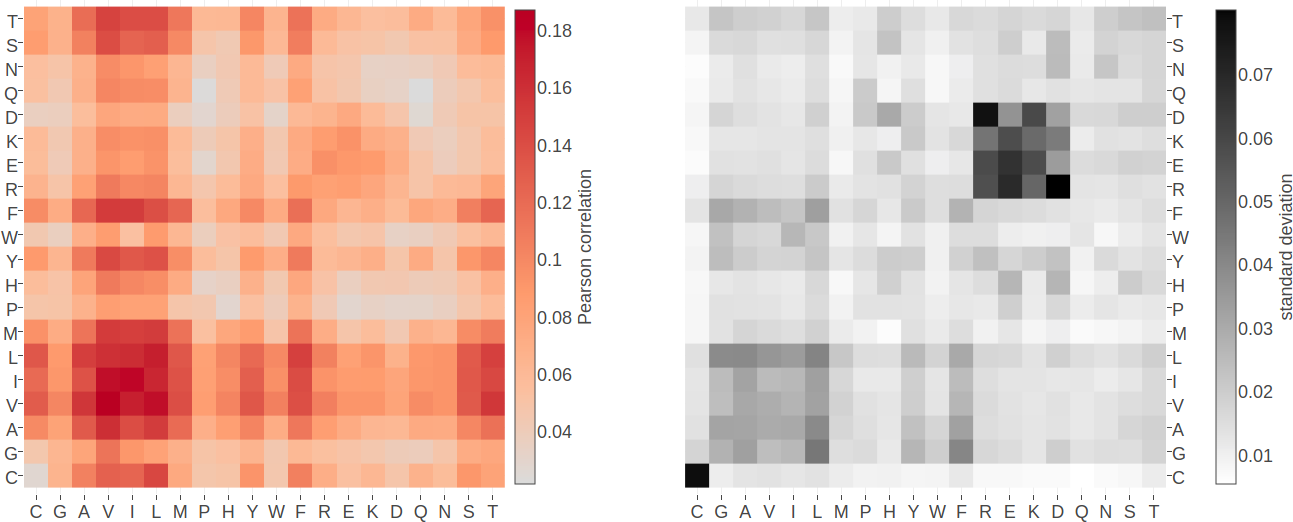
\includegraphics[width=1\linewidth]{img/coupling_matrix_analysis/combi_squared_couplings_correlation_and_stddev_heatmap_notitle} 

}

\caption{\textbf{Left} Pearson correlation of squared
coupling values \((\wijab)^2\) with contact class (contact=1,
non-contact=0). \textbf{Right} Standard deviation of squared coupling
values. Dataset contains 100.000 residue pairs per class (for details
see methods section \ref{method-coupling-correlation}). Amino acids are
abbreviated with one-letter code and they are broadly grouped with
respect to physico-chemical properties listed in Appendix
\ref{amino-acids}.}\label{fig:sq-coupling-correlation}
\end{figure}

Different couplings are of varying importance for contact inference and
have distinct characteristics. When looking at the raw coupling values
(without squaring), these charateristics become even more pronounced.
The left plot in Figure \ref{fig:coupling-correlation} shows the
correlation of raw coupling values \(\wijab\) with contact class.
Interestingly, in contrast to the findings for squared coupling values,
couplings for charged residue pairs, involving arginine (R), glutamic
acid (E), lysine (K) and aspartic acid (D), have the strongest class
correlation (positive and negative), whereas aliphatic coupling pairs
correlate to a much lesser extent. This implies that squared coupling
value is a better indicator of a contact than the raw signed coupling
value for aliphatic couplings. On the contrary, the raw signed coupling
values for charged residue pairs are much more indicative of a contact
than the magnitude of their squared values. Raw couplings for cysteine
(C-C) pairs, proline (P) and tryptophane (W) correlate only weakly with
contact class. For these pairs neither a squared coupling value nor the
raw coupling value seems to be a good indicator for a contact.









\begin{figure}
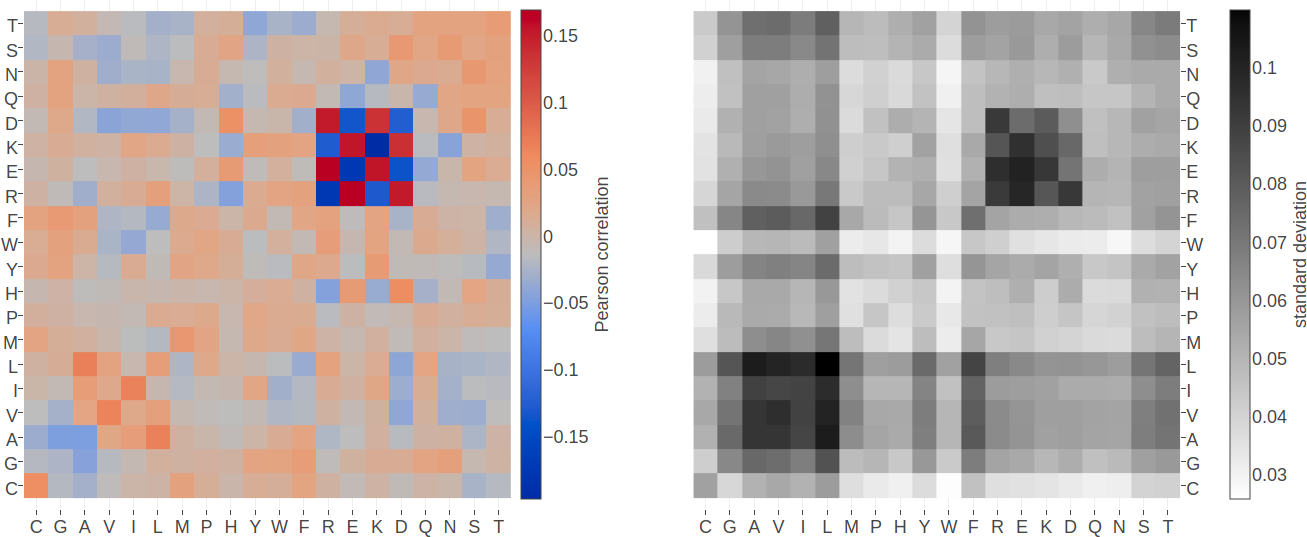
\includegraphics[width=1\linewidth]{img/coupling_matrix_analysis/combi_couplings_correlation_and_stddev_heatmap_notitle} \caption{\textbf{Left} Pearson correlation of
raw signed coupling values \(\wijab\) with contact class (contact=1,
non-contact=0). \textbf{Right} Standard deviation of coupling values.
Dataset contains 100.000 residue pairs per class (for details see
section \ref{method-coupling-correlation}). Amino acids are abbreviated
with one-letter code and they are broadly grouped with respect to
physico-chemical properties listed in Appendix \ref{amino-acids}.}\label{fig:coupling-correlation}
\end{figure}

Looking only at correlations can be misleading if there are non-linear
patterns in the data, for example higher order dependencies between
couplings. For this reason it is advisable to take a more detailed view
at coupling matrices and the distributions of their values.

\section{Physico-Chemical Fingerprints in Coupling
Matrices}\label{physico-chemical-fingerprints-in-coupling-matrices}

The correlation analysis of coupling matrices in the last section
revealed that certain couplings are more indicative of a contact than
others. Individual coupling matrices for a residue pair that is in
physcial contact often display striking patterns that agree with the
previous findings. These patterns allow a biological interpreation of
the coupling values that reveal details of the physico-chemical
interdependency between both residues.

Figure \ref{fig:coupling-matrix-ionic-interaction} visualizes the
inferred coupling matrix for a residue pair using the pseudo-likelihood
method. A cluster of strong coupling values can be observed for the
couplings between the charged residues glutamic acid (E), aspartic acid
(D), lysine (K) and arginine (R) and the polar residue glutamine (Q).
Positive coupling values arise between positively charged residues (K,
R) and negatively charged residues (E, D), whereas couplings between
equally charged residues have negative values. These exemplary couplings
(E-R, E-K, K-D) perfectly reflect the interaction preference for
residues forming salt bridges. Indeed, in the protein structure the
first residue (E) forms a salt bridge with the second residue (R) as can
be seen in the left plot in Figure \ref{fig:coupling-matrix-pymol}.











\begin{figure}
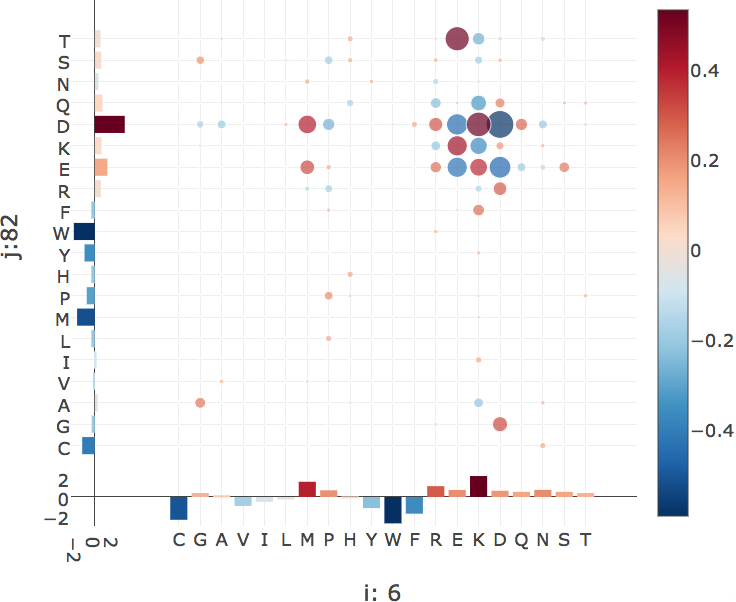
\includegraphics[width=0.9\linewidth]{img/coupling_matrix_analysis/coupling_matrix_1a9xA05_6_82_notitle} \caption{Coupling matrix computed
with pseudo-likelihood for residues 6 and 82 in protein chain
1a9x\_A\_05. Color represents coupling strength and direction (red =
positive coupling value, blue = negative coupling value) and diameter of
bubbles represents absolute coupling value \(|\wijab|\). Bars at the
x-axis and y-axis correspond to the \emph{Potts model} single potentials
\(\vi\) and \(\vj\). Amino acids are abbreviated with one-letter code
and they are broadly grouped with respect to physico-chemical properties
listed in Appendix \ref{amino-acids}.}\label{fig:coupling-matrix-ionic-interaction}
\end{figure}

Figure \ref{fig:coupling-matrix-hydrophobic-interaction} visualizes the
coupling matrix for a pair of hydrophobic residues. Hydrophobic
pairings, such as alanine (A) - isoleucine (I), or glycine (G) -
isoleucine (I) have strong coupling values but the couplings also
reflect a sterical constraint. Alanine is a small hydrophobic residue
and it is favoured at both residue positions because it has strong
positive couplings with isoleucine (I), leucine (L) and methionine (M).
But alanine is disfavoured to appear at both positions at the same time
as the A-A coupling is negative. Figure \ref{fig:coupling-matrix-pymol}
illustrates the location of the two residues in the protein core. Here,
hydrophobic residues are densely packed and the limited space allows for
only small hydrophobic residues.











\begin{figure}
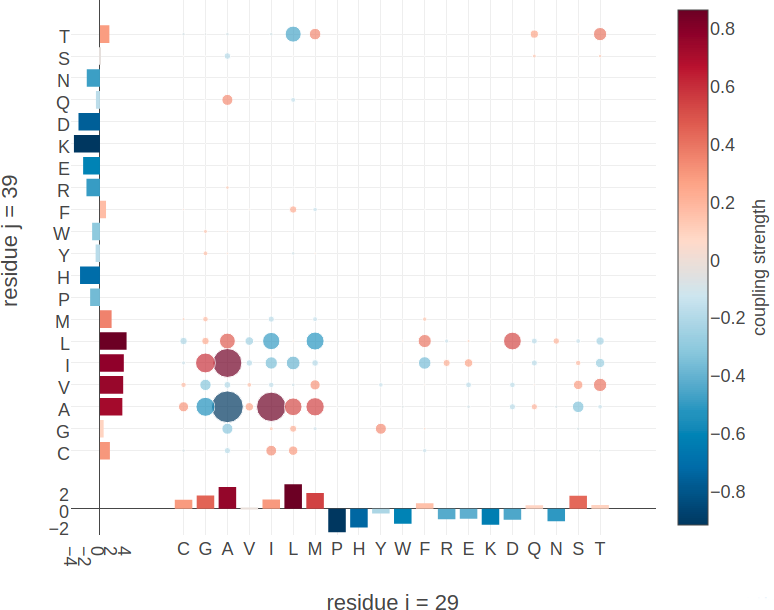
\includegraphics[width=0.9\linewidth]{img/coupling_matrix_analysis/coupling_matrix_1ae9A00_29_39_notitle} \caption{Coupling matrix
computed with pseudo-likelihood for residues 29 and 39 in protein chain
1ae9\_A\_00. Color represents coupling strength and direction (red =
positive coupling value, blue = negative coupling value) and diameter of
bubbles represents absolute coupling value \(|\wijab|\). Bars at the
x-axis and y-axis correspond to the \emph{Potts model} single potentials
\(\vi\) and \(\vj\). Amino acids are abbreviated with one-letter code
and they are broadly grouped with respect to physico-chemical properties
listed in Appendix \ref{amino-acids}.}\label{fig:coupling-matrix-hydrophobic-interaction}
\end{figure}






\begin{figure}
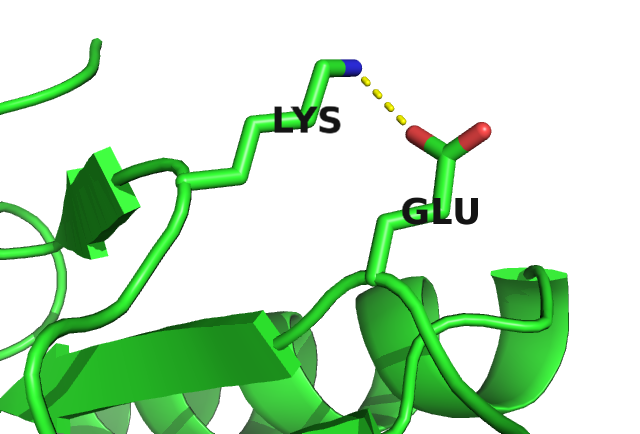
\includegraphics[width=0.5\linewidth]{img/coupling_matrix_analysis/1a9xA05_6_82} 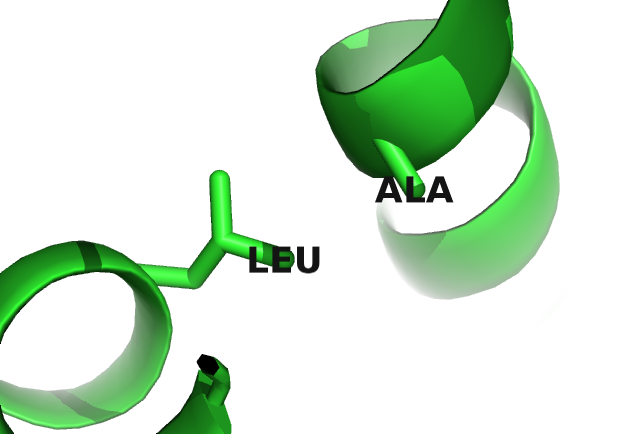
\includegraphics[width=0.5\linewidth]{img/coupling_matrix_analysis/1ae9A00_29_39} \caption{Interactions between protein side
chains. \textbf{Left}: residue 6 (E) forms a salt bridge with residue 82
(R) in protein chain 1a9x\_A\_05. \textbf{Right}: residue 29 (A) and
residue 39 (L) within the hydrophobic core of protein chain 1ae9\_A\_00.}\label{fig:coupling-matrix-pymol}
\end{figure}

Many more biological interpretable signals can be identified from
coupling matrices, including pi-cation interactions (see Appendix
\ref{pi-cation}), aromatic-proline interactions (see Appendix
\ref{aromatic-proline}), sulfur-aromatic interactions or disulphide
bonds (see Appendix \ref{disulfide}).

Coucke and collegues performed a thorough quantitative analysis of
coupling matrices selected from confidently predicted residue pairs
{[}\protect\hyperlink{ref-Coucke2016}{1}{]}. They showed that eigenmodes
obtained from a spectral analysis of averaged coupling matrices are
closely related to physico-chemical properties of amino acid
interactions, like electrostaticity, hydrophobicity, steric interactions
or disulphide bonds. By looking at specific populations of residues,
like buried and exposed residues or residues from specific protein
classes (small, mainly \(\alpha\), etc), the eigenmodes of corresponding
coupling matrices are found to capture very characteristic interactions
for each class, e.g.~rare disulfide contacts within small proteins and
hydrophilic contacts between exposed residues. Their study confirms the
qualitative observations presented above that amino acid interactions
can leave characteristic physico-chemical fingerprints in coupling
matrices.

\section{Coupling Profiles Vary with
Distance}\label{coupling-profiles-vary-with-distance}

Analyses in the previous sections showed that certain coupling values
correlate more or less strong with contact class and that coupling
matrices for contacts express biological meaningfull patterns.

More insights can be obtained by looking at the distribution of distinct
coupling values for contacts, non-contacts and arbitrary populations of
residue pairs. Figure \ref{fig:1d-coupling-profile-0-5} shows the
distribution of selected couplings for filtered residue pairs with
\(\Cb-\Cb\) distances \(< 5\angstrom\) (see methods section
\ref{method-coupling-profile} for details). The distribution of R-E and
E-E coupling values is shifted and skewed towards positive and negative
values respectively. This is in accordance with attracting electrostatic
interactions between the positively charged side chain of arginine and
the negatively charged side chain of gluatamic acid and also with
repulsive interactions between the two negatively charged glutamic acid
side chains. Coupling values for cysteine pairs (C-C) have a broad
distribution that is skewed towards positive values, reflecting the
strong signals obtained from covalent disulphide bonds. The broad
distribution for C-C, R-E and E-E agrees with the observation in section
\ref{correlation-between-couplings-and-class} that these specific
coupling values have large standard deviations and that for charged
residue pairings the signed coupling value is a strong indicator of a
contact.

Hydrophobic pairs like V-I have an almost symmetric coupling
distribution, confirming the finding that the direction of coupling is
not indicative of a true contact whereas the strength of the coupling
is. The hydrophobic effect that determines hydrophobic interactions is
not specific or directed. Therefore, hydrophobic interaction partners
can commonly be substituted by other hydrophobic residues, which
explains the not very pronounced positive coupling signal compared to
more specific interactions, e.g ionic interactions. The distribution of
aromatic coupling values like F-W is slightly skewed towards negative
values, accounting for steric hindrance of their large side chains at
small distances.










\begin{figure}

{\centering 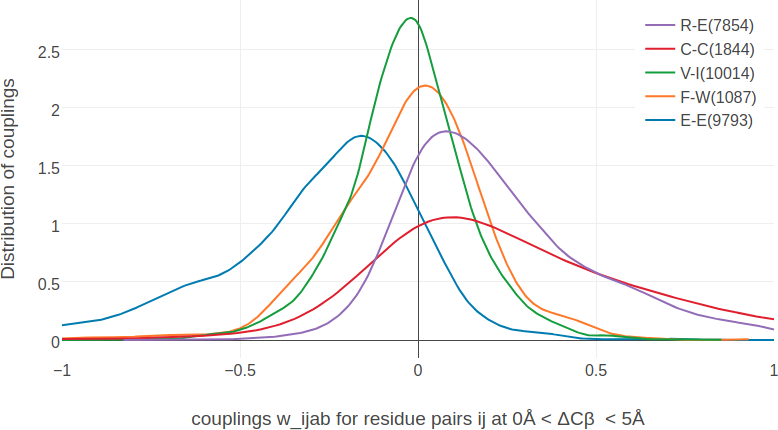
\includegraphics[width=0.9\linewidth]{img/coupling_matrix_analysis/1d_coupling_profile_0_5} 

}

\caption{Distribution of selected couplings
for filtered residue pairs with \(\Cb-\Cb\) distances \(< 5\angstrom\)
(see methods section \ref{method-coupling-profile} for details). Number
of coupling values used to determine the distribution is given in
brackets in the legend. R-E = couplings for arginine and glutamic acid
pairs, C-C = coupling for cystein residue pairs, V-I = coupling for
valine and isoleucine pairs, F-W = coupling for phenylalanine and
tryptophane pairs, E-E = coupling for glutamic acid residue pairs.}\label{fig:1d-coupling-profile-0-5}
\end{figure}

In an intermediate \(\Cb\) distance range between \(8\angstrom\) and
\(12\angstrom\) the distributions for all coupling values are centered
close to zero and are less broad. The distributions are still shifted
and skewed, but less pronounced compared to the distributions at
\(\Cb-\Cb\) distances \(< 5\angstrom\). For aromatic pairs like F-W, the
distribution of coupling values has very long tails, suggesting rare but
strong couplings for aromatic side chains at this distance.








\begin{figure}
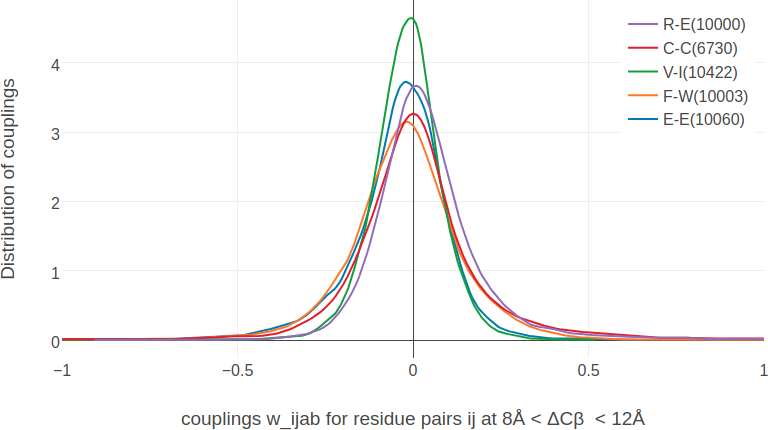
\includegraphics[width=1\linewidth]{img/coupling_matrix_analysis/1d_coupling_profile_8_12} \caption{Distribution of selected
couplings for filtered residue pairs with \(\Cb-\Cb\) distances between
\(8\angstrom\) and \(12 \angstrom\) (see methods section
\ref{method-coupling-profile} for details). Number of coupling values
used to determine the distribution is given in brackets in the legend.
Couplings are the same as in Figure \ref{fig:1d-coupling-profile-0-5}.}\label{fig:1d-coupling-profile-8-12}
\end{figure}

Figure \ref{fig:1d-coupling-profile-20-50} shows the distribution of
selected couplings for residue pairs far apart in the protein structure
(\(\Cb-\Cb\) distances \(> 20\angstrom\)).\\
The distribution for all couplings is centered at zero and has small
variance. Only for C-C coupling values, the distribution has a long tail
for positve values, presumably arising from the fact that the maximum
entropy model cannot distuinguish highly conserved signals of multiple
disulphide bonds within a protein. This observation also agrees with the
previous finding in section
\ref{correlation-between-couplings-and-class} that C-C coupling values,
albeit having large standard-deviations, correlate only weakly with
contact class. The same arguments apply to couplings of aromatic pairs
that have a comparably broad distribution and do not correlate strongly
with the contact class. The strong coevolution signals for aromatic
pairs even at high distance ranges might result from transitive effects
that could not be completely resolved by the \emph{Potts model}.
Aromatic residues are known to form network-like structures in the
protein core that stabilize protein structure and can lead to transitive
effects (see Figure \ref{fig:aromatic-network} in
Appendix){[}\protect\hyperlink{ref-Burley1985}{2}{]}.








\begin{figure}
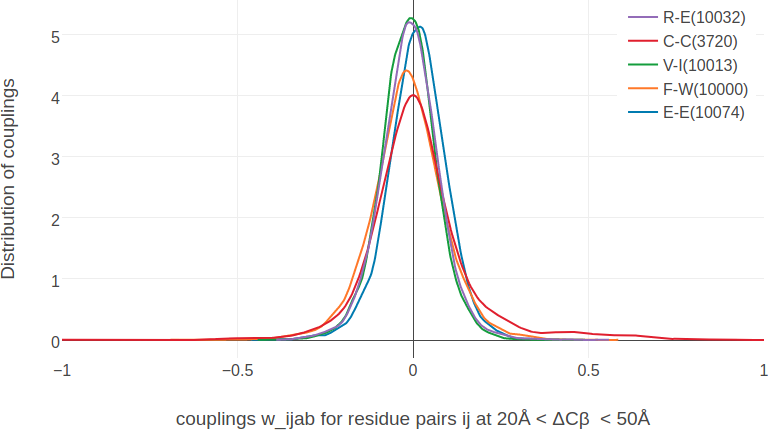
\includegraphics[width=1\linewidth]{img/coupling_matrix_analysis/1d_coupling_profile_20_50} \caption{Distribution of selected
couplings for filtered residue pairs with \(\Cb-\Cb\) distances between
\(20\angstrom\) and \(50\angstrom\) (see methods section
\ref{method-coupling-profile} for details). Number of coupling values
used to determine the distribution is given in brackets in the legend.
Couplings are the same as in Figure \ref{fig:1d-coupling-profile-0-5}.}\label{fig:1d-coupling-profile-20-50}
\end{figure}

\section{Higher Order Dependencies Between
Couplings}\label{higher-order-dependencies-between-couplings}

The analyses in the previous sections focused on single coupling values
picked from the \(20 \times 20\)-dimensional coupling matrices \(\wij\).
As mentioned before, analysing only single dimensions might be
misleading when variables are dependent on each other and further
insights might be concealed in higher order relationships.
Unfortunately, it is not possible to reasonably visualize high
dimensional coupling matrices.

Exploring two dimensional coupling scatter plots strengthens the
observation that couplings matrices contain signals that reflect
biological relevant amino acid interactions. The plots in the top row in
Figure \ref{fig:2d-coupling-profiles-0-8} show the distribution of
couplings for filtered residue pairs with \(\Cb-\Cb\) distances
\(< 8\angstrom\) between the ionic pairings of E-R and R-E and between
the ionic pairing R-E and the equally charged residues E-E,
respectively. Coupling values for R-E and E-R are positively correlated
with predominantly positive values. This means when the amino acid pair
R-E is frequently observed at two positions \(i\) and \(j\), then it
also likely that the amino acid pair E-R can be frequently observed.
This situation indicates an important ionic interaction whereby the
location of the positively and negatively charged residue at position
\(i\) or \(j\) is irrelevant.

On the contrary, coupling values for R-E and E-E are negatively
correlated, with positive values for R-E and negative values for E-E.
This distribution can be interpreted with frequently occuring amino acid
pairs R-E at two positions \(i\) and \(j\) while at the same time the
amino acid pair E-E cannot be observed. Again, this situation coincides
with amino acid pairings that would be expected for an ionic
interaction.

The bottom left plot in Figure \ref{fig:2d-coupling-profiles-0-8} shows
the distribution between couplings for the hydrophobic pairings I-L and
V-I that is almost symmetric and broadly centered around zero. Coupling
distributions for residue pairs that are not physically interacting
(\(\Cb \gg 8 \angstrom\)) resemble the distribution for hydrophobic
pairings in that there is no correlation, but at high distance the
distributions are much tighter centered around zero (bottom right plot
in Figure \ref{fig:2d-coupling-profiles-0-8}).
















\begin{figure}
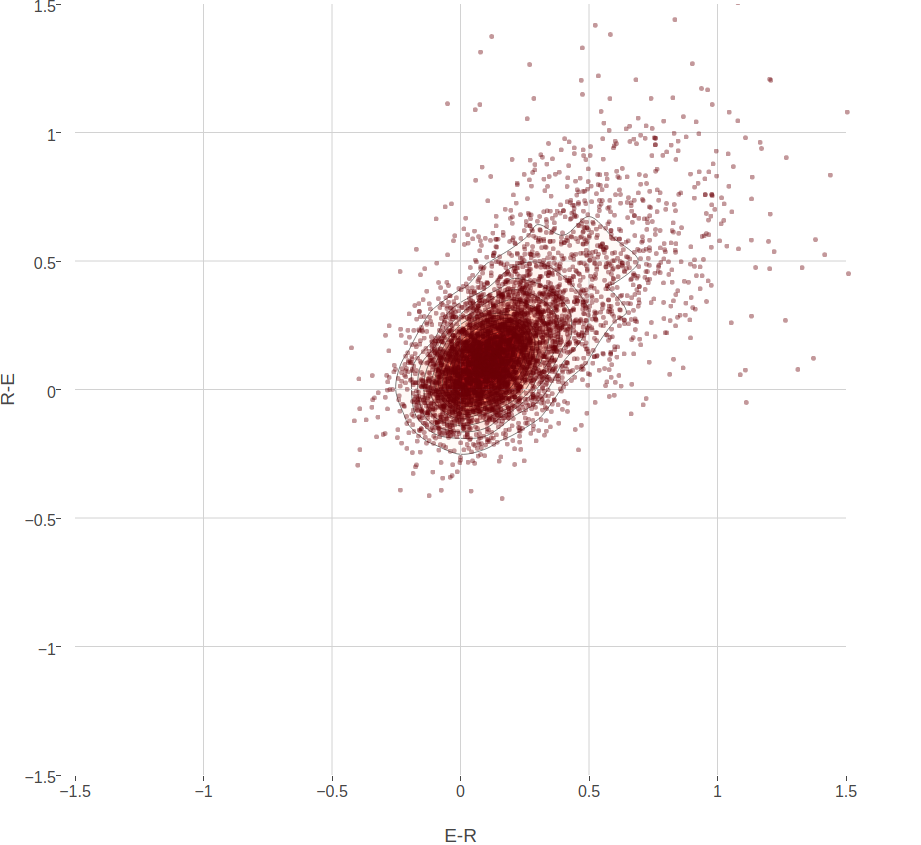
\includegraphics[width=0.5\linewidth]{img/coupling_matrix_analysis/pairwise_couplings_R-E_E-R_Cbdistance_0_8_notitle} 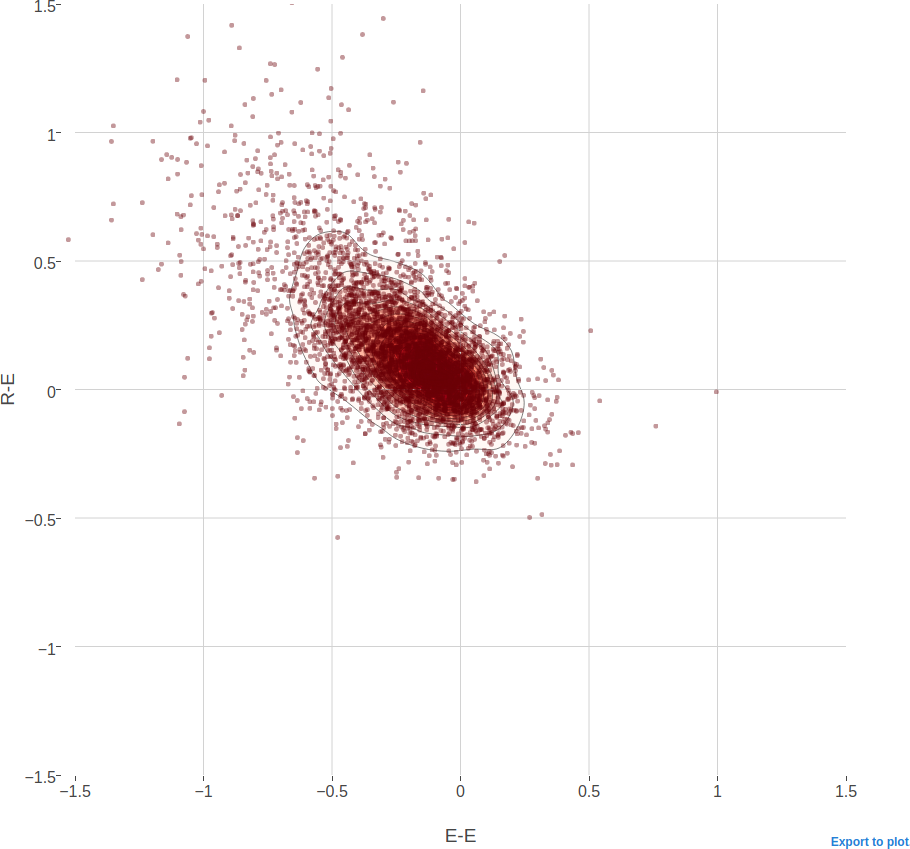
\includegraphics[width=0.5\linewidth]{img/coupling_matrix_analysis/pairwise_couplings_R-E_E-E_Cbdistance_0_8_notitle} 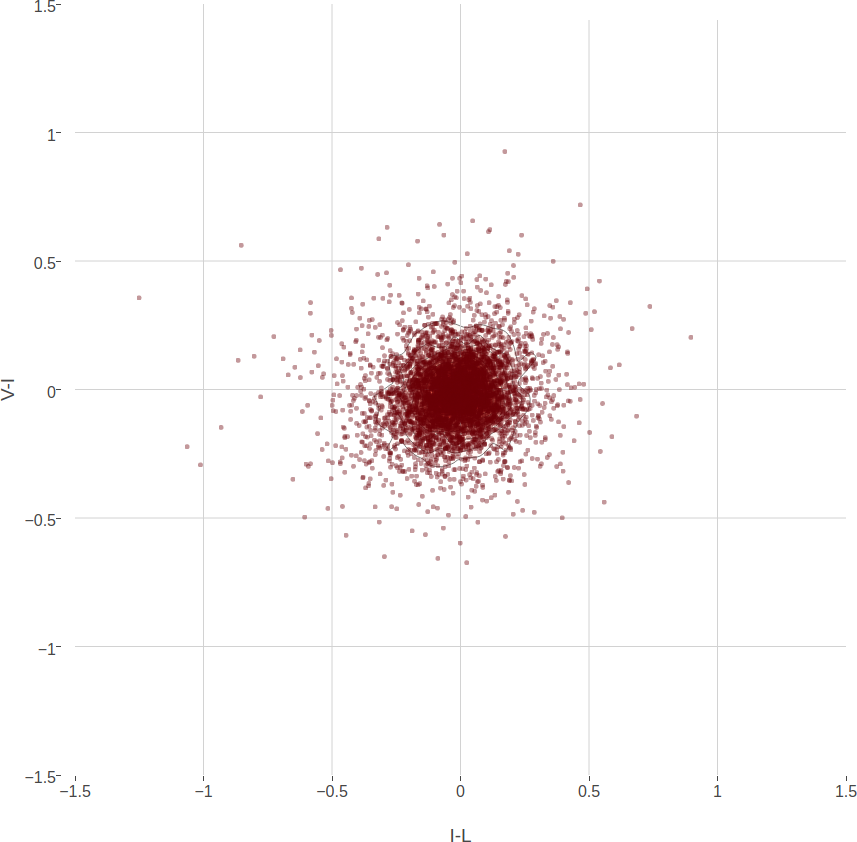
\includegraphics[width=0.5\linewidth]{img/coupling_matrix_analysis/pairwise_couplings_V-I_I-L_Cbdistance_0_8_notitle} 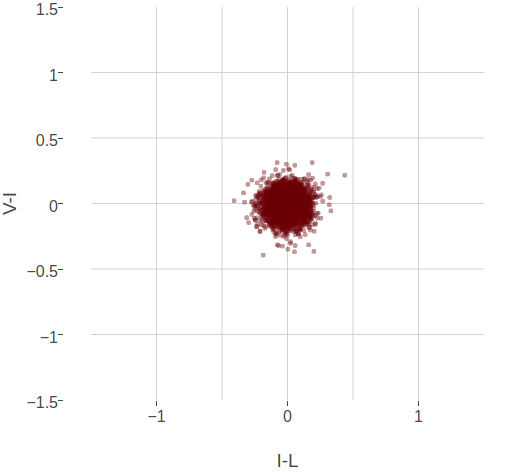
\includegraphics[width=0.5\linewidth]{img/coupling_matrix_analysis/pairwise_couplings_V-I_I-L_Cbdistance_20_50_notitle} \caption{Two-dimensional distribution of
approximately 10000 coupling values computed with pseudo-likelihood.
\textbf{Top Left} The 2-dimensional distribution of couplings E-R and
R-E for residue pairs with \(\Cb-\Cb\) distances \(< 8 \angstrom\) is
almost symmetric and the coupling values are positively correlated.
\textbf{Top Right} The 2-dimensional distribution of couplings E-R and
E-E for residue pairs with \(\Cb-\Cb\) distances \(< 8 \angstrom\) is
almost symmetric and the coupling values are negatively correlated.
\textbf{Bottom Left} The 2-dimensional distribution of couplings I-L and
V-I for residue pairs with \(\Cb-\Cb\) distances \(< 8 \angstrom\) is
symmetrically distributed around zero without visible correlation.
\textbf{Bottom Right} The 2-dimensional distribution of couplings I-L
and V-I for residue pairs with \(\Cb-\Cb\) distances \(> 20 \angstrom\)
is tighly distributed around zero. .}\label{fig:2d-coupling-profiles-0-8}
\end{figure}

\chapter{Contact Prior}\label{contact-prior}

The wealth of successful meta-predictors presented in section
\ref{meta-predictors} highlights the importance to exploit other sources
of information apart from coevolution statistics. Much information about
residue interactions is typically contained in single position features
that can be predicted from local sequence profiles, such as secondary
structure, solvent accessibility or contact number, and in pairwise
features such as the contact prediction scores for residue pairs
\((i,j)\) from a simple local statistical methods as presented in
section \ref{local-methods}.

For example, predictions of secondary structure elements and solvent
accessibility are used by almost all modern machine learning predictors,
such as MetaPsicov {[}\protect\hyperlink{ref-Jones2015a}{3}{]}, NeBCon
{[}\protect\hyperlink{ref-He2017}{4}{]}, EPSILON-CP
{[}\protect\hyperlink{ref-Stahl2017}{5}{]}, PconsC3
{[}\protect\hyperlink{ref-Skwark2016}{6}{]}. Other frequently used
sequence derived features include pairwise contact potentials, sequence
separation and conservation measures such as column entropy
{[}\protect\hyperlink{ref-Jones2015a}{3},\protect\hyperlink{ref-He2017}{4},\protect\hyperlink{ref-Ma2015a}{7}{]}.

In the following sections I present a random forest classifier that uses
sequence derived features to distinguish contacts from non-contacts.
Methods section \ref{seq-features} lists all features used to train the
classifier including the aforementioned standard features as well as
some novel features.

The probabilistic predictions of the random forest model can be
introduced directly as prior information into the Bayesian statistical
model presented in the last section \ref{bayesian-approach} to improve
the overall prediction accuracy in terms of posterior probabilities.
Furthermore, contact scores from coevolution methods can be added as
additional feature to the random forest model in order to elucidate how
much the combined information improves prediction accuracy over the
single methods.

\section{Random Forest Classifiers}\label{random-forest-classifiers}

Random Forests are supervised machine learning methods that belong to
the class of ensemble methods
{[}\protect\hyperlink{ref-Ho1998}{8}--\protect\hyperlink{ref-Breiman2001}{10}{]}.
They are easy to implement, fast to train and can handle large numbers
of features due to implicit feature selection
{[}\protect\hyperlink{ref-Menze2009}{11}{]}.

Ensemble methods combine the predictions of several independent base
estimators with the goal to improve generalizability over a single
estimator. Random forests are ensembles of decision trees where
randomness is introduced in two ways:

\begin{enumerate}
\def\labelenumi{\arabic{enumi}.}
\tightlist
\item
  every tree is build on a random sample that is drawn with replacement
  from the training set and has the same size as the training set (i.e.,
  a bootstrap sample)
\item
  every split of a node is evaluated on a random subset of features
\end{enumerate}

A single decision tree, especially when it is grown very deep is highly
susceptible to noise in the training set and therefore prone to
overfitting which results in poor generalization ability. As a
consequence of randomness and averaging over many decision trees, the
variance of a random forest predictor decreases and therefore the risk
of overfitting {[}\protect\hyperlink{ref-Louppe2014}{12}{]}. It is still
advisable to restrict the depth of single trees in a random forest, not
only to counteract overfitting but also to reduce model complexity and
to speedup the algorithm.

Random forests are capable of regression and classification tasks. For
classification, predictions for new data are obtained by running each
data sample down every tree in the forest and then either apply majority
voting over single class votes or averaging the probabilistic class
predictions. Probabilistic class predictions of single trees are
computed as the fraction of training set samples of the same class in a
leaf whereas the single class vote refers to the majority class in a
leaf. Figure \ref{fig:rf-intro} visualizes the procedure of classifying
a new data sample.









\begin{figure}

{\centering 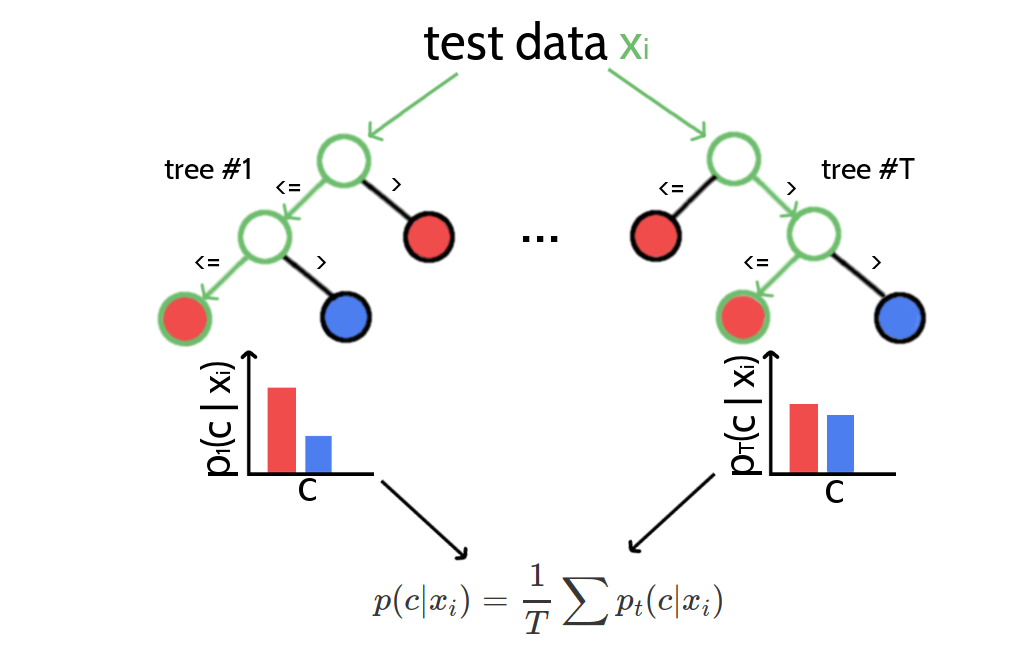
\includegraphics[width=0.8\linewidth]{img/random_forest_contact_prior/intro_random_forest} 

}

\caption{Classifying new data with random forests. A new
data sample is run down every tree in the forest until it ends up in a
leaf node. Every leaf node has associated class probabilities \(p(c)\)
reflecting the fraction of training samples belonging to every class
\(c\). The color of the leaf nodes reflects the class with highest
probability. The predictions from all trees in form of the class
probabilties are averaged over all trees and yield the final prediction.}\label{fig:rf-intro}
\end{figure}

Typically, \emph{Gini impurity}, which is a computationally efficient
approximation to the entropy, is used as a split criterion to evaluate
the quality of a split. It measures the degree of purity in a data set
regarding class labels as \(GI = (1 - \sum_{k=1}^K p_k^2)\), where
\(p_k\) is the proportion of class \(k\) in the data set. For every
feature \(f\) in the random subset that is considered for splitting a
particular node \(N\), the \emph{decrease in Gini impurity}
\(\Delta GI_f\) will be computed as,

\[
\Delta GI_f(N_{\textrm{parent}}) = GI_f(N_{\textrm{parent}}) - p_{\textrm{left}} GI_f(N_{\textrm{left}}) - p_{\textrm{right}} GI_f(N_{\textrm{left}})
\]

where \(p_{\textrm{left}}\) and \(p_{\textrm{right}}\) refers to the
fraction of samples ending up in the left and right child node
respectively {[}\protect\hyperlink{ref-Menze2009}{11}{]}. The feature
\(f\) with highest \(\Delta GI_f\) over the two resulting child node
subsets will be used to split the data set at the given node \(N\).

Summing the \emph{decrease in Gini impurity} for a feature \(f\) over
all trees whenever \(f\) was used for a split yields the \emph{Gini
importance} measure, which can be used as an estimate of general feature
relevance. Random forests therefore are popular methods for feature
selection and it is common practice to remove the least important
features from a data set to reduce the complexity of the model. However,
feature importance measured with respect to \emph{Gini importance} needs
to be interpreted with care. The random forest model cannot distinguish
between correlated features and it will choose any of the correlated
features for a split, thereby reducing the importance of the other
features and introducing bias. Furthermore, it has been found that
feature selection based on \emph{Gini importance} is biased towards
selecting features with more categories as they will be chosen more
often for splits and therefore tend to obtain higher scores
{[}\protect\hyperlink{ref-Strobl2007}{13}{]}.

\section{Evaluating Random Forest Model as Contact
Predictor}\label{evaluating-random-forest-model-as-contact-predictor}

I trained a random forest classifier on the feature set described in
methods section \ref{seq-features} and optimized model hyperparameters
as well as some data set specific settings (e.g window size and class
ratios) with 5-fold cross-validation as described in methods section
\ref{rf-hyperparameter-optimization}.

Figure \ref{fig:rf-feature-importance} shows the ranking of the ten most
important features according to \emph{Gini importance}. Both local
statistical contact scores, \emph{OMES}
{[}\protect\hyperlink{ref-Fodor2004a}{14}{]} and
\protect\hyperlink{abbrev}{MI} (mutual information between amino acid
counts), constitute the most important features besides the mean pair
potentials acording to Miyazawa \& Jernigan
{[}\protect\hyperlink{ref-Miyazawa1999a}{15}{]} and
Li\&Fang{[}\protect\hyperlink{ref-Li2011}{16}{]}. Further important
features include the relative solvent accessibility at both pair
positions, the total percentage of gaps at both positions, the
correlation between mean isoelectric point property at both positions,
sequence separation and the beta-sheet propensity in a window of size
five around position i.
























\begin{figure}
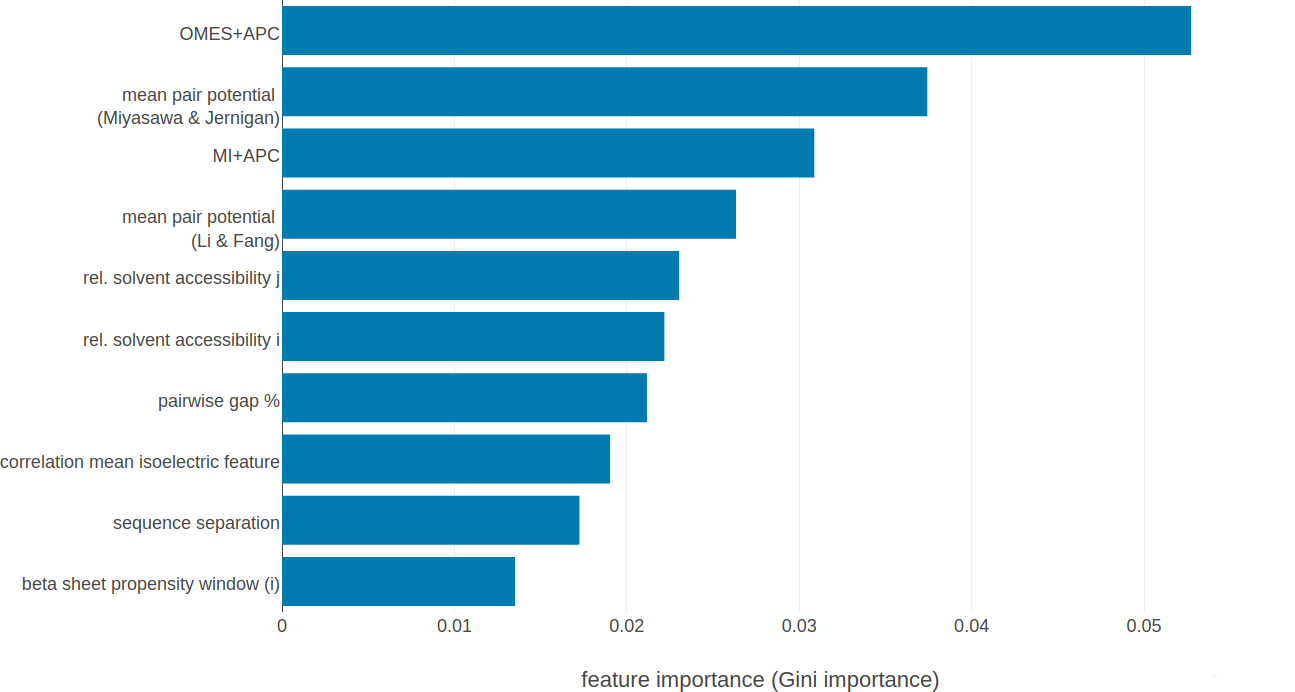
\includegraphics[width=1\linewidth]{img/random_forest_contact_prior/feature_random_forest_optimalhyperparameters_topfeatures} \caption{Top ten features ranked according to
\emph{Gini importance}. \textbf{OMES+APC}:
\protect\hyperlink{abbrev}{APC} corrected OMES score according to
Fodor\&Aldrich {[}\protect\hyperlink{ref-Fodor2004a}{14}{]}.
\textbf{mean pair potential (Miyasawa \& Jernigan)}: average
quasi-chemical energy of transfer of amino acids from water to the
protein environment {[}\protect\hyperlink{ref-Miyazawa1999a}{15}{]}.
\textbf{MI+APC}: \protect\hyperlink{abbrev}{APC} corrected mutual
information between amino acid counts (using pseudo-counts).
\textbf{mean pair potential (Li\&Fang)}: average general contact
potential by Li \& Fang {[}\protect\hyperlink{ref-Li2011}{16}{]}.
\textbf{rel. solvent accessibilty i(j)}: RSA score computed with
Netsurfp (v1.0) {[}\protect\hyperlink{ref-Petersen2009a}{17}{]} for
position i(j). \textbf{pairwise gap\%}: percentage of gapped sequences
at either position i and j. \textbf{correlation mean isoelectric
feature}: Pearson correlation between the mean isoelectric point feature
(according to Zimmermann et al., 1968) for positions i and j.
\textbf{sequence separation}: \textbar{}j-i\textbar{}. \textbf{beta
sheet propensity window(i)}: beta-sheet propensity according to Psipred
{[}\protect\hyperlink{ref-Jones1999}{18}{]} computed within a window of
five positions around i. eatures are described in detail in methods
section \ref{seq-features}.}\label{fig:rf-feature-importance}
\end{figure}

Many features have low \emph{Gini importance} scores which means they
are rarely considered for splitting a node and can likely be removed
from the dataset. Removing irrelevant features from the dataset is a
convenient procedure to reduce model complexity. As described in methods
section \ref{rf-feature-selection}, I performed feature selection by
evaluating model performance on subsets of features of decreasing
importance. Most models trained on subsets of the total feature space
perform nearly identical compared to the model trained on all features,
as can be seen in Figure \ref{fig:rf-feature-selection-performance}.
Performance of the random forest models drops noticeably when using only
the 25 most important features. For the further analysis I am using the
random forest model trained on the 75 most important features as this
model constitutes the smallest set of features while performing nearly
identical compared to the model trained on the complete feature set.







\begin{figure}
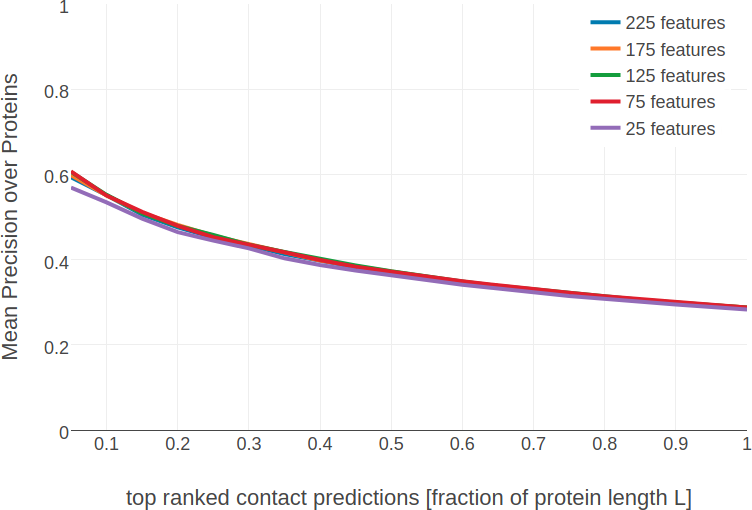
\includegraphics[width=1\linewidth]{img/random_forest_contact_prior/precision_vs_rank_featureselection_random_forest_optimized_hyperparameters} \caption{Mean precision of top
ranked predictions over 200 proteins for random forest models trained on
subsets of features of decreasing importance. Subsets of features have
been selected as described in methods section
\ref{rf-feature-selection}.}\label{fig:rf-feature-selection-performance}
\end{figure}

Figure \ref{fig:performance-rf} shows the mean precision for the random
forest model trained on the 75 most important features. The random
forest model has a mean precision of 0.33 for the top \(0.5\cdot L\)
contacts compared to a precision of 0.47 for pseudo-likelihood.
Furthermore, the random forest model improves approximately ten
percentage points in precision over the local statistical contact
scores, \emph{OMES} and mutual information (MI). Both methods comprise
important features of the random forest model as can be seen in Figure
\ref{fig:rf-feature-importance}.

When analysing performance with respect to alignment size it can be
found that the random forest model outperforms the pseudo-likelihood
score for small alignments (see Figure \ref{fig:performance-neff-rf}).\\
Both, local statistial models \emph{OMES} and
\protect\hyperlink{abbrev}{MI} also perform weak on small alignments,
leading to the conclusion that the remaining sequence derived features
are highly relevant when the alignment contains only few sequences. This
finding is expected, as it is well known that models trained on simple
sequence features perform almost independent of alignment size
{[}\protect\hyperlink{ref-Stahl2017}{5}{]}.














\begin{figure}
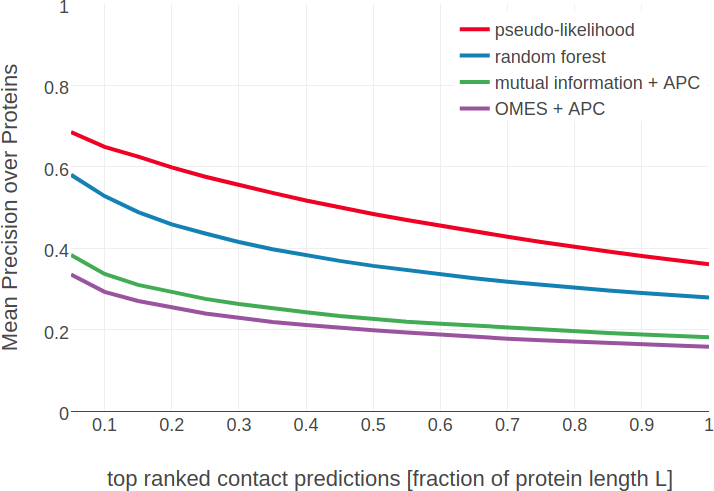
\includegraphics[width=1\linewidth]{img/random_forest_contact_prior/precision_vs_rank_notitle} \caption{Mean precision for top ranked contacts on a
test set of 774 proteins. \textbf{random forest (pLL)} = random forest
model using sequence derived features and pseudo-likelihood contact
score (\protect\hyperlink{abbrev}{APC} corrected Frobenius norm of
couplings). \textbf{pseudo-likelihood} = \protect\hyperlink{abbrev}{APC}
corrected Frobenius norm of couplings computed with pseudo-likelihood.
\textbf{random forest} = random forest model trained on 75 sequence
derived features. \textbf{OMES} = \protect\hyperlink{abbrev}{APC}
corrected \emph{OMES} contact score according to Fodor\&Aldrich
{[}\protect\hyperlink{ref-Fodor2004a}{14}{]}. \textbf{mutual
information} = \protect\hyperlink{abbrev}{APC} corrected mutual
information between amino acid counts (using pseudo-counts).}\label{fig:performance-rf}
\end{figure}























\begin{figure}
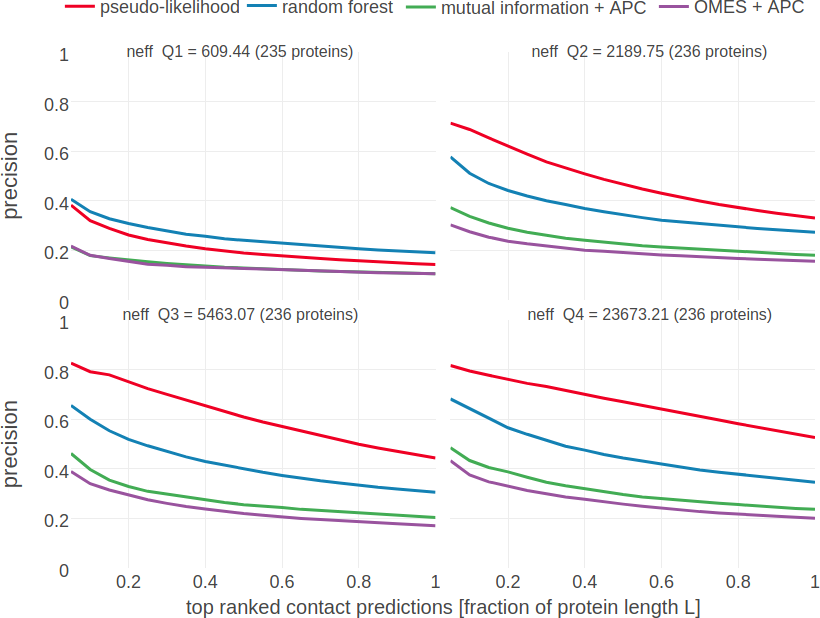
\includegraphics[width=1\linewidth]{img/random_forest_contact_prior/precision_vs_rank_facetted_by_neff_notitle} \caption{Mean precision for top ranked contacts
on a test set of 774 proteins splitted into four equally sized subsets
with respect to \protect\hyperlink{abbrev}{Neff}. Subsets are defined
according to quantiles of \protect\hyperlink{abbrev}{Neff} values. Upper
left: Subset of proteins with \protect\hyperlink{abbrev}{Neff}
\textless{} Q1. Upper right: Subset of proteins with Q1 \textless{}=
\protect\hyperlink{abbrev}{Neff} \textless{} Q2. Lower left: Subset of
proteins with Q2 \textless{}= \protect\hyperlink{abbrev}{Neff}
\textless{} Q3. Lower right: Subset of proteins with Q3 \textless{}=
\protect\hyperlink{abbrev}{Neff} \textless{} Q4. \textbf{random forest
(pLL)} = random forest model using sequence derived features and
pseudo-likelihood contact score (\protect\hyperlink{abbrev}{APC}
corrected Frobenius norm of couplings). \textbf{pseudo-likelihood} =
\protect\hyperlink{abbrev}{APC} corrected Frobenius norm of couplings
computed with pseudo-likelihood. \textbf{random forest} = random forest
model trained on 75 sequence derived features. \textbf{OMES} =
\protect\hyperlink{abbrev}{APC} corrected \emph{OMES} contact score
according to Fodor\&Aldrich
{[}\protect\hyperlink{ref-Fodor2004a}{14}{]}. \textbf{mutual
information} = \protect\hyperlink{abbrev}{APC} corrected mutual
information between amino acid counts (using pseudo-counts).}\label{fig:performance-neff-rf}
\end{figure}

Figure \ref{fig:performance-neff-rf} showed that the random forest
predictor improves over the pseudo-likelihood coevolution method when
the alignment consists of only few sequences. In order to assess this
improvement in a more direct manner, it is possible to build a combined
random forest predictor that is not only trained on the sequence derived
features but also on the pseudo-likelihood contact score as an
additional feature (see methods section \ref{rf-with-pll-score} for
details). As expected, the pseudo-likelihood score comprises the most
important feature in the model (Figure
\ref{fig:feature-importance-rf-with-pll-score} in methods section)
followed by the same sequence features that were found in the previous
analysis in Figure \ref{fig:rf-feature-importance}.

Finally, comparing the random forest model trained on sequence features
and pseudo-likelihood contact score to the pseudo-likelihood score in
Figure \ref{fig:performance-rf} reveals that combining both types of
information indeed improves predictive power over both single
approaches. Especially for small alignments, the improvement is
substantial as can be seen in in the left upper plot in Figure
\ref{fig:performance-neff-rf}. In contrast, the improvement on large
alignments (right lower plot in Figure \ref{fig:performance-neff-rf}) is
small, as the gain from simple sequence features compared to the much
more powerful coevolution signals is neglectable.

\chapter{Methods}\label{methods}

all you need to know

\section{Dataset}\label{dataset}

A protein dataset has been constructed from the CATH (v4.1)
{[}\protect\hyperlink{ref-Sillitoe2015}{19}{]} database for
classification of protein domains. All CATH domains from classes
1(mainly \(\alpha\)), 2(mainly \(\beta\)), 3(\(\alpha+\beta\)) have been
selected and filtered for internal redundancy at the sequence level
using the \texttt{pdbfilter} script from the
HH-suite{[}\protect\hyperlink{ref-Remmert2012}{20}{]} with an E-value
cutoff=0.1. The dataset has been split into ten subsets aiming at the
best possible balance between CATH classes 1,2,3 in the subsets. All
domains from a given CATH topology (=fold) go into the same subsets, so
that any two subsets are non-redundant at the fold level. Some
overrepresented folds (e.g.~Rossman Fold) have been subsampled ensuring
that in every subset each class contains at max 50\% domains of the same
fold. Consequently, a fold is not allowed to dominate a subset or even a
class in a subset. In total there are 6741 domains in the dataset.

Multiple sequence alignments were built from the CATH domain sequences
(\href{http://www.cathdb.info/version/current/domain/3cdjA03/sequence}{COMBS})
using HHblits {[}\protect\hyperlink{ref-Remmert2012}{20}{]} with
parameters to maximize the detection of homologous sequences:

\texttt{hhblits\ -maxfilt\ 100000\ -realign\_max\ 100000\ -B\ 100000\ -Z\ 100000\ -n\ 5\ -e\ 0.1\ -all}
\texttt{hhfilter\ -id\ 90\ -neff\ 15\ -qsc\ -30}

The COMBS sequences are derived from the SEQRES records of the PDB file
and sometimes contain extra residues that are not resolved in the
structure. Therefore, residues in PDB files have been renumbered to
match the COMBS sequences. The process of renumbering residues in PDB
files yielded ambigious solutions for 293 proteins, that were removed
from the dataset. Another filtering step was applied to remove 80
proteins that do not hold the following properties:

\begin{itemize}
\tightlist
\item
  more than 10 sequences in the multiple sequence alignment (\(N>10\))
\item
  protein length between 30 and 600 residues (\(30 \leq L \leq 600\))
\item
  less than 80\% gaps in the multiple sequence alignment (percent gaps
  \textless{} 0.8)
\item
  at least one residue-pair in contact at \(C_\beta < 8\angstrom\) and
  minimum sequence separation of 6 positions
\end{itemize}

The final dataset is comprised of \textbf{6368} proteins with almost
evenly distributed CATH classes over the ten subsets (Figure
\ref{fig:dataset-cath-topologies}).





\begin{figure}
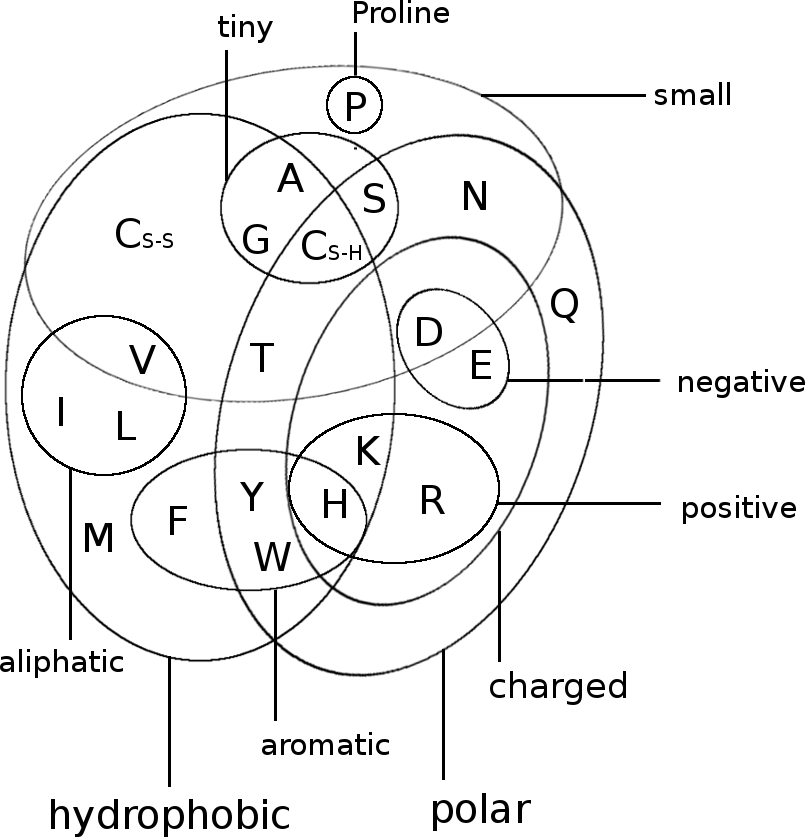
\includegraphics[width=1\linewidth]{img/amino_acid_physico_chemical_properties_venn_diagramm} \caption{Distribution of CATH classes
(1=mainly \(\alpha\), 2=mainly \(\beta\), 3=\(\alpha-\beta\)) in the
dataset and the ten subsets. }\label{fig:dataset-cath-topologies}
\end{figure}

\section{Optimizing
Pseudo-Likelihood}\label{optimizing-pseudo-likelihood}

Dr Stefan Seemayer has reimplementated the open-source software CCMpred
{[}\protect\hyperlink{ref-Seemayer2014}{21}{]} in Python. Based on a
fork of his private github repository I continued development and
extended the software, which is now called CCMpredPy. It will soon be
available at \url{https://github.com/soedinglab/CCMpredPy}. All
computations in this thesis are performed with CCMpredPy unless stated
otherwise.

\subsection{Pseudo-Likelihood Objective Function and its
Gradients}\label{pseudo-likelihood-objective-function-and-its-gradients}

CCMpred optimizes the regularized negative pseudo-log-likelihood using
conjugate gradients optimizer.

The negative pseudo-log-likelihood, abbreviated \(\mathcal{npll}\), is
defined as:

\begin{equation}
  \mathcal{npll}(\mathbf{X} | \v,\w) =   - \sum_{n=1}^N \sum_{i=1}^L  \left(  v_i(x_i^{(n)}) + \sum_{\substack{j=1 \\ j \neq i}}^L w_{ij}(x_i^{(n)}, x_j^{(n)})  - \log Z_i^{(n)} \right)
\end{equation}

The normalization term \(Z_i\) sums over all assignments to one position
\(i\) in sequence:

\begin{equation}
  Z_i^{(n)} = \sum_{a=1}^{20} \exp \left( v_i(a) + \sum_{\substack{j=1 \\ j \neq i}}^L w_{ij}(a, x_j^{(n)}) \right)
\end{equation}

\subsection{Differences between CCMpred and
CCMpredpy}\label{diff-ccmpred-ccmpredpy}

CCMpredPy differs from CCMpred
{[}\protect\hyperlink{ref-Seemayer2014}{21}{]} which is available at
\url{https://github.com/soedinglab/CCMpred} in several details:

\begin{itemize}
\tightlist
\item
  Initialization of potentials \(\v\) and \(\w\)

  \begin{itemize}
  \tightlist
  \item
    CCMpred initializes single potentials
    \(\v_i(a) = \log f_i(a) - \log f_i(a= "-")\) with \(f_i(a)\) being
    the frequency of amino acid a at position i and \(a="-"\)
    representing a gap. A single pseudo-count has been added before
    computing the frequencies. Pair potentials \(\w\) are intialized at
    0.
  \item
    CCMpredPy initializes single potentials \(\v\) with the
    \protect\hyperlink{abbrev}{ML} estimate of single potentials (see
    section \ref{regularization}) using amino acid frequencies computed
    as described in section \ref{amino-acid-frequencies}. Pair
    potentials \(\w\) are initialized at 0.
  \end{itemize}
\item
  Regularization

  \begin{itemize}
  \tightlist
  \item
    CCMpred uses a Gaussian regularization prior centered at zero for
    both single and pair potentials. The regularization coefficient for
    single potentials \(\lambda_v = 0.01\) and for pair potentials
    \(\lambda_w = 0.2 * (L-1)\) with \(L\) being protein length.
  \item
    CCMpredPy uses a Gaussian regularization prior centered at zero for
    the pair potentials. For the single potentials the Gaussian
    regularization prior is centered at the
    \protect\hyperlink{abbrev}{ML} estimate of single potentials (see
    section \ref{regularization}) using amino acid frequencies computed
    as described in section \ref{amino-acid-frequencies}. The
    regularization coefficient for single potentials \(\lambda_v = 10\)
    and for pair potentials \(\lambda_w = 0.2 * (L-1)\) with \(L\) being
    protein length.
  \end{itemize}
\end{itemize}

Default settings for CCMpredPy have been chosen to best reproduce
CCMpred results. A benchmark over a subset of approximately 3000
proteins confirms that performance measured as
\protect\hyperlink{abbrev}{PPV} for both methods is almost identical
(see Figure \ref{fig:cmmpredvanilla-vs-ccmpredpy}).









\begin{figure}
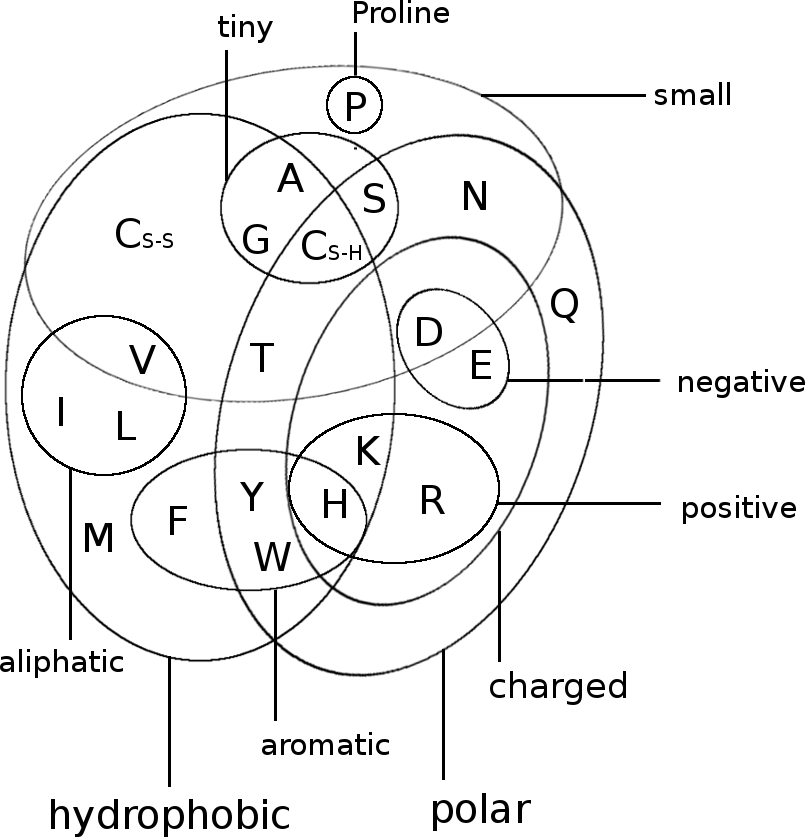
\includegraphics[width=1\linewidth]{img/amino_acid_physico_chemical_properties_venn_diagramm} \caption{Benchmark for CCMpred and
CCMpredPy on a dataset of 3124 proteins. ccmpred-vanilla+apc: CCMpred
{[}\protect\hyperlink{ref-Seemayer2014}{21}{]} with
\protect\hyperlink{abbrev}{APC}. ccmpred-pll-centerv+apc: CCMpredPy with
\protect\hyperlink{abbrev}{APC}. Specific flags that have been used to
run both methods are described in detail in the text (see section
\ref{diff-ccmpred-ccmpredpy}).}\label{fig:cmmpredvanilla-vs-ccmpredpy}
\end{figure}

The benchmark in Figure \ref{fig:cmmpredvanilla-vs-ccmpredpy} as well as
all contacts predicted with CCMpred and CCMPredPy (using
pseudo-likelihood) in my thesis have been computed using the following
flags:

Flags used with CCMpredPy (using pseudo-likelihood objective function):

\begin{verbatim}
--maxit 250                       # Compute a maximum of MAXIT operations
--center-v                        # Use a Gaussian prior for single potentials centered at ML estimate v*
--reg-l2-lambda-single 10         # regularization coefficient for single potentials
--reg-l2-lambda-pair-factor 0.2   # regularization coefficient for pairwise potentials computed as reg-l2-lambda-pair-factor * (L-1)
--pc-uniform                      # use uniform pseudocounts (1/21 for 20 amino acids + 1 gap state) 
--pc-count 1                      # defining pseudo count admixture coefficient rho = pc-count/( pc-count+ Neff)
--epsilon 1e-5                    # convergence criterion for minimum decrease in the last K iterations
--ofn-pll                         # using pseudo-likelihood as objective function
--alg-cg                          # using conjugate gradient to optimize objective function
\end{verbatim}

Flags used with CCMpred:

\begin{verbatim}
-n 250    # NUMITER:  Compute a maximum of NUMITER operations
-l 0.2    # LFACTOR:  Set pairwise regularization coefficients to LFACTOR * (L-1) 
-w 0.8    # IDTHRES:  Set sequence reweighting identity threshold to IDTHRES
-e 1e-5   # EPSILON:  Set convergence criterion for minimum decrease in the last K iterations to EPSILON
\end{verbatim}

\subsection{Sequence Reweighting}\label{seq-reweighting}

As discussed in section \ref{challenges}, sequences in a
\protect\hyperlink{abbrev}{MSA} do not represent independent draws from
a probabilistic model. To reduce the effects of overrepresented
sequences, typically a simple weighting strategy is applied that assigns
a weight to each sequence that is the inverse of the number of similar
sequences according to an identity threshold
{[}\protect\hyperlink{ref-Stein2015a}{22}{]}. It has been found that
reweighting improves contact prediction performance
{[}\protect\hyperlink{ref-Buslje2009}{23}--\protect\hyperlink{ref-Jones2012}{25}{]}
significantly but results are robust against the choice of the identity
threshold in a range between 0.7 and 0.9
{[}\protect\hyperlink{ref-Morcos2011}{24}{]}. We chose an identity
threshold of 0.8.

Every sequence \(x_n\) of length \(L\) in an alignment with \(N\)
sequences has an associated weight \(w_n = 1/m_n\), where \(m_n\)
represents the number of similar sequences:

\begin{equation} 
  w_n = \frac{1}{m_n}, m_n = \sum_{m=1}^N I \left( ID(x_n, x_m) \geq 0.8 \right) \\
  ID(x_n, x_m)=\frac{1}{L} \sum_{i=1}^L I(x_n^i = x_m^i)
  \label{eq:seqweight}
\end{equation}

The number of effective sequences \(\mathbf{\neff}\) of an alignment is
then the number of sequence clusters computed as:

\begin{equation} 
  \neff = \sum_{n=1}^N w_n
  \label{eq:neff}
\end{equation}

TODO: Plot Performance for Seq weighting

\subsection{Computing Amino Acid
Frequencies}\label{amino-acid-frequencies}

Single and pairwise amino acid frequencies are computed from the
alignment by weighting amino acid counts (see section
\ref{seq-reweighting}) and adding pseudocounts for numerical stability.

Let \(a,b \in \{1,\ldots,20\}\) be amino acids,
\(q(x_i=a), q(x_i=a, x_j=b)\) and \(q_0(x_i=a), q_0(x_i=a,x_j=b)\) be
the empirical single and pair frequencies with and without pseudocounts,
respectively. We define

\begin{align}
    q(x_i \eq a) :=& (1-\tau) \;  q_0(x_i \eq a) + \tau \tilde{q}(x_i\eq a) \\
    q(x_i \eq a, x_j \eq b) :=& (1-\tau)^2  \; [ q_0(x_i \eq a, x_j \eq b) - q_0(x_i \eq a)  q_0(x_j \eq b) ] + \\
                            & q(x_i \eq a) \; q(x_j \eq b) 
\label{eq:pseudocounts}
\end{align}

with \(\tilde{q}(x_i \eq a) := f(a)\) being background amino acid
frequencies and \(\tau \in [0,1]\) is a pseudocount admixture
coefficient, which is a function of the diversity of the multiple
sequence alignment:

\begin{equation}
    \tau = \frac{N_\mathrm{pc}}{(N_\mathrm{eff} + N_\mathrm{pc})}
\label{eq:tau}
\end{equation}

where \(N_{pc} > 0\).

The formula for \(q(x_i \eq a, x_j \eq b)\) in the second line in eq
\eqref{eq:pseudocounts} was chosen such that for \(\tau \eq0\) we obtain
\(q(x_i \eq a, x_j \eq b) = q_0(x_i \eq a, x_j \eq b)\), and furthermore
\(q(x_i \eq a, x_j \eq b) = q(x_i \eq a) q(x_j \eq b)\) exactly if
\(q_0(x_i \eq a, x_j \eq b) = q_0(x_i \eq a) q_0(x_j \eq b)\).

\section{Analysis of Coupling
Matrices}\label{analysis-of-coupling-matrices}

\subsection{Correlation of Couplings with Contact
Class}\label{method-coupling-correlation}

Approximately 100000 residue pairs have been filtered for contacts and
non-contacts respectively according to the following criteria:

\begin{itemize}
\tightlist
\item
  consider only residue pairs separated by at least 10 positions in
  sequence
\item
  minimal diversity (\(=\frac{\sqrt{N}}{L}\)) of alignment = 0.3
\item
  minimal number of non-gapped sequences = 1000
\item
  \(\Cb\) distance threshold for contact: \(<8\angstrom\)
\item
  \(\Cb\) distance threshold for noncontact: \(>25\angstrom\)
\end{itemize}

\subsection{Coupling Distribution Plots}\label{method-coupling-profile}

For one-dimensional coupling distribution plots the residue pairs and
respective pseudo-log-likelihood coupling values \(\wijab\) have been
selected as follows:

\begin{itemize}
\tightlist
\item
  consider only residue pairs separated by at least 10 positions in
  sequence
\item
  discard residues that have more than 30\% gaps in the alignment
\item
  discard residue pairs that have insufficient evidence in the
  alignment: \(N_{ij} \cdot q_i(a) \cdot q_j(b) < 100\) with:

  \begin{itemize}
  \tightlist
  \item
    \(N_{ij}\) is the number of sequences with neither a gap at position
    i nor at position j
  \item
    \(q_i(a)\) and \(q_j(b)\) are the frequencies of amino acids a and b
    at positions i and j (computed as described in section
    \ref{amino-acid-frequencies})
  \end{itemize}
\end{itemize}

These criteria ensure that uninformative couplings are neglected,
e.g.~sequence neighbors albeit being contacts according to the \(\Cb\)
contact definition cannot be assumed to express biological meaningful
coupling patterns, or couplings for amino acid pairings that do not have
statistical relevant counts in the alignment.

The same criteria have been applied for selecting couplings for the
two-dimensional distribution plots with the difference that evidence for
a single coupling term has to be
\(N_{ij} \cdot q_i(a) \cdot q_j(b) < 80.\)

\section{Optimizing the
Full-Likelihood}\label{methods-optimizing-full-likelihood}

The following sections will describe the hyperparameter tuning for the
stochastic gradient descent optimization as well as tuning different
aspects of the Gibbs sampling scheme used to approximate the gradient
with \protect\hyperlink{abbrev}{CD}.

In theory the algorithm has converged and the optimum of the objective
function has been reached when the gradient becomes zero. In practice
the gradients will never be exactly zero, especially due to the
stochasticity of the gradient estimates when using stochastic gradient
descent.

For this reason, usually some kind of convergence criterion is designed
and convergence is assumed whenever the criterion is met. A common
criterion is the when the relative change of objective function value
between iterations is close to zero. However, because the evaluation of
the full likelihood function is too expensive, the function value cannot
be used to define a criterion.

Another possibility is to stop learning when the norm of the gradient is
close to zero {[}\protect\hyperlink{ref-Carreira-Perpinan2005}{26}{]}.
For \protect\hyperlink{abbrev}{CD} however, the gradients will be far
off zero depending on how many sequences are used for sampling. Only
when sampling large number of sequences, the gradients will eventually
be close to zero (see section @ref(sampling more seq)). This is however
achieved at the expense of runtine which increases linearly in the
number of sequences for sampling.

An alternative is to check the relative change over the norm of
gradients between iterations and stop the algorithm whenever it falls
below a small threshold \(\epsilon\),

\begin{equation}
  \frac{|\nabla_\theta f(\theta_{t-1}) - \nabla_\theta f(\theta_{t})|}{|\nabla_\theta f(\theta_{t-1})|}  < \; \epsilon \; .
  \label{eq:gradient-convergence-criterion}
\end{equation}

However, as gradient estimates are very noisy for stochastic gradient
descent, gradient fluctuations complicate the proper assessment of this
criterion. It is also possible to monitor the relative change over the
norm of parameter estimates between iterations,

\begin{equation}
  \frac{|\theta_{t-1} - \theta_t|}{|\theta_t|}  < \; \epsilon  \; .
  \label{eq:parameter-convergence-criterion}
\end{equation}

This criterion is more stable as parameter updates are dampened by the
step size are not quite as noisy compared to subsequent gradient
estimates.

Another idea is to monitor the direction of gradients. Once getting
close to the optimum, gradients will start to fluctuate as the optimizer
will oscillate around the true optimum. From my experience, it is hard
to find a general threshold that applies to all proteins, as every
protein reflects a problem of varying complexity (number of parameters
scales with \(L^2\), L being protein length). Furthermore this analysis
is complicated when using momentum, as the computed gradient is not
actually used to change the parameters but it is combined with previous
gradient estimates.

A necessary but not sufficient criterion for convergence is given by
\(\sum_{a,b=1}^{20} \wijab = 0\) as derived in section \ref{prior-v}.
When using plain stochastic gradient descent without momentum and
without adaptive learning rates, this criterion is never violated when
parameters are initialized uniformly. This is due to the fact that the
400 gradients \(\wijab\) for \(a,b \in \{1, \ldots, 20\}\) are not
independent. The sum over the 400 pairwise amino acid counts for two
positions i and j is identical for the observed and sampled alignment,

\begin{equation}
  \sum_{a,b=1}^{20} N_{ij} q(x_i \eq a, q_j \eq b) = N_{ij} \; ,
\end{equation}

and therefore the gradients, computed as the difference of pairwise
counts between observed and sampled alignment, are symmetrical.
Considering residue pair (i,j) and assuming amino acid pair (a,b) has
higher counts in the sampled alignment compared to the true alignment,
then this differnce in counts must be compensated by other amino acid
pairs (c,d) having less counts in the sampled alignment compared to the
true alignment. This symmetry is translated into parameter updates when
the same learning rate is used to update all parameters. However, when
using adaptive learning rates, this symmetry is broken and the condition
\(\sum_{a,b=1}^{20} \wijab = 0\) can be violated during the optimization
processs. It is therefore interesting to monitor
\(\sum_{1 \le 1 < j \le L} \sum_{a,b=1}^{20} \wijab\).

Finally, the simplest strategy is to specify a maximum number of
iterations for the optimization procedure. This also ensures that the
algorithm will stop eventually if none of the other convergence criteria
is met.

In the following, I will set the maximum number of iterations to 5000
and I will stop the optimization when the relative change over the norm
of parameter estimates falls below the threshold of \(\epsilon = 1e-8\).
Furthermore, I will follow the pragmatic standard strategy and run the
optimization algorithm with many hyperparameter settings and pick the
model that gives the best performance on a validation set
{[}\protect\hyperlink{ref-Le2011}{27}{]}.

The performance will be evaluated as the mean precision of the top
ranked contact predictions over a benchmark set of 300 proteins, that is
a subset of the data set described in methods section \ref{dataset}.
Pseudo-likelihood couplings are computed with the tool CCMpredPy that is
introduced in methods section \ref{diff-ccmpred-ccmpredpy}. Contact
scores for couplings obtained with pseudo-likelihood and
\protect\hyperlink{abbrev}{CD} are computed as the
\protect\hyperlink{abbrev}{APC} corrected Frobenius norm as explained in
section \ref{post-processing-heuristics}.

Coupling parameters are initialized at 0.

\subsection{\texorpdfstring{Full Likelihood Optimization with
\emph{ADAM}}{Full Likelihood Optimization with ADAM}}\label{methods-full-likelihood-adam}

\emph{ADAM} {[}\protect\hyperlink{ref-Kingma2014}{28}{]} stores an
exponentially decaying average of past gradients and squared gradients,

\begin{align}
  m_t &= \beta_1 m_{t−1} + (1 − \beta_1) g \\
  v_t &= \beta_2 v_{t−1} + (1 − \beta_2) g^2 \; ,
\end{align}

with \(g = \nabla_w \LLreg(\v,\w)\) and the rate of decay being
determined by hyperparameters \(\beta_1\) and \(\beta_2\). Both terms
\(m_t\) and \(v_t\) represent estimates of the first and second moments
of the gradient, respectively.

The full Adam update also includes a bias correction mechanism, which
compensates for the fact that in the first few time steps the vectors
m,v are both initialized and therefore biased at zero, before they fully
``warm up''. Because \(m_t\) and \(v_t\) are initialized as vectors of
zeros, the following bias correction terms are supposed to counteract
the initialization bias towards zero,

\begin{align}
  \hat{m_t} &= \frac{m_t}{1-\beta_1^t} \\
  \hat{v_t} &= \frac{v_t}{1-\beta_2^t} \; .
\end{align}

Parameters are then updated using step size \(\alpha\), a small noise
term \(\epsilon\) and the corrected moment estimates \(\hat{m_t}\),
\(\hat{v_t}\), according to

\begin{equation}
  x_{t+1} = x_t - \alpha \cdot \frac{\hat{m_t}}{\sqrt{\hat{v_t}} + \epsilon}
\end{equation}

Kingma et al. proposed the default values \(\beta_1=0.9\),
\(\beta_2=0.999\) and \(\epsilon=1e−8\) and a constant learning rate
\(\alpha_0=1e-3\), because \emph{ADAM} performs a kind of step size
annealing by nature. However, popular implementations of \emph{ADAM} in
the
\href{https://github.com/fchollet/keras/blob/master/keras/optimizers.py\#L385}{Keras}
{[}\protect\hyperlink{ref-Chollet2015}{29}{]} and
\href{https://github.com/Lasagne/Lasagne/blob/master/lasagne/updates.py\#L565-L629}{Lasagne}
{[}\protect\hyperlink{ref-Dieleman2015}{30}{]} packages allow the use of
a linear annealing schedule for the learning rate \(\alpha\) of the form
\(\alpha = \frac{\alpha_0}{1 + \gamma t}\), for an initial learning rate
\(\alpha_0\), decay rate \(\gamma\) and timestep \(t\).

I first tested three different constant learning rates
\(\alpha \in \{1e-4, 1e-3, 5e-3\}\) and default parameters
\(\beta_1=0.9\), \(\beta_2=0.999\) and \(\epsilon=1e−8\).

PLOT

As can be seen in the performance: not goot. Looking at individual
proteins:

\subsection{Full Likelihood Optimization with Stochastic Gradient
Descent}\label{full-likelihood-optimization-with-stochastic-gradient-descent}

The coupling parameters \(\w\) will be updated in each iteration \(t\)
by taking a step of size \(\alpha\) along the direction of the negative
gradient of the regularized full log likelihood
\(- \nabla_w \LLreg(\v,\w)\) that has been approximated with
\protect\hyperlink{abbrev}{CD},

\begin{equation}
  \w_{t+1} = \w_t - \alpha \cdot \nabla_w \LLreg(\v,\w) \; .
\end{equation}

In order to get a first intuition of the optimization problem, I tested
initial learning rates
\(\alpha_0 \in \{1\mathrm{e}{-4}, 5\mathrm{e}{-4}, 1\mathrm{e}{-3}, 5\mathrm{e}{-3}\}\)
with a standard learning rate annealing schedule,
\(\alpha = \frac{\alpha_0}{1 + \gamma \cdot t}\) with decay rate
\(\gamma=0.01\) and timestep \(t\)
{[}\protect\hyperlink{ref-Bottou2012}{31}{]}.

Figure \ref{fig:performance-cd-alphaopt} shows the mean precision for
top ranked contacts computed from pseudo-likelihood couplings and the
\protect\hyperlink{abbrev}{CD} couplings optimized with stochastic
gradient descent using the four different learning rates. Overall, mean
precision for \protect\hyperlink{abbrev}{CD} contacts is smaller than
for pseudo-likelihood contacts. Especially the smallest
(\(1\mathrm{e}{-4}\)) and biggest learning (\(5\mathrm{e}{-3}\)) rate
perform bad.










\begin{figure}

{\centering 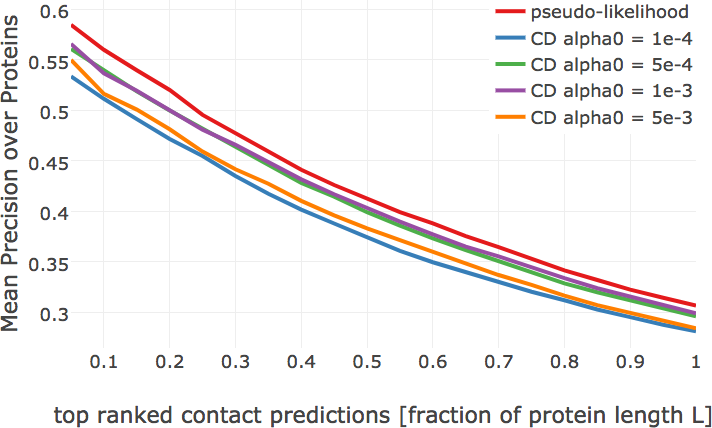
\includegraphics[width=0.9\linewidth]{img/full_likelihood/sgd/precision_vs_rank_learning_rates} 

}

\caption{Mean precision for top ranked
contact predictions over 286 proteins. Contact scores are computed as
the \protect\hyperlink{abbrev}{APC} corrected Frobenius norm of the
couplings \(\wij\). pseudo-likelihood: Contact scores computed from
pseudo-likelihood. The other methods derive contact scores from
couplings computed from \protect\hyperlink{abbrev}{CD} using stochastic
gradient descent with different initial learning rates \(\alpha_0\) as
specified in the legend.}\label{fig:performance-cd-alphaopt}
\end{figure}

Looking at individual proteins it turns out that the optimal learning
rate depends on alignment size. Figure
\ref{fig:sgd-single-proteins-initial-learning-rate} shows convergence
plots for two different proteins, where convergence is measured as the
L2-norm of coupling parameters \(||\w||_2\). For an exemplary protein
with a small alignment (left plot in Figure
\ref{fig:sgd-single-proteins-initial-learning-rate}), a small learning
rate \(1\mathrm{e}{-4}\) lets the optimization run very slowly and not
reach convergence within 5000 iterations. A large learning rate of
\(5\mathrm{e}{-3}\) overshoots the optimum at the beginning of the
optimization but as the learning rate decays over time the parameter
estimates converge. In contrast, for a protein with a big alignment
(right plot in Figure
\ref{fig:sgd-single-proteins-initial-learning-rate}) the learning rate
choice has a more pronounced effect. With a small initial learning rate
of \(1\mathrm{e}{-4}\) the optimization runs slowly but almost converges
within 5000 iterations. A large initial learning rate of
\(5\mathrm{e}{-3}\) lets the parameters diverge quickly and the optimum
cannot be revovered. With learning rates \(5\mathrm{e}{-4}\) and
\(1\mathrm{e}{-3}\), the optimum is well overshot at the beginning of
the optimization but the parameter estimates eventually converge as the
learning rates decreases over time.

These observations are explained by the fact that the magnitude of the
gradient scales with the number of sequences in the alignment. Because
the gradient is computed from amino acid counts (see section
\ref{full-likelihood-gradient}), alignments with many sequences will
generally produce larger gradients compared to alignments with few
sequences, especially at the beginning of the optimization procedure
when the difference in amino acid counts between sampled and observed
sequences is largest. Following these observation,s I defined the
initial learning rate \(\alpha_0\) as a function of
\protect\hyperlink{abbrev}{Neff}.\\
Aiming to obtain values for \(\alpha_0\) around 5e-3 for small
\protect\hyperlink{abbrev}{Neff} and values for \(\alpha_0\) around 1e-4
for large \protect\hyperlink{abbrev}{Neff}, the initial learning rate is
defined as

\begin{equation}
  \alpha_0 = \frac{5\mathrm{e}{-2}}{\sqrt{N_{\text{eff}}}} \; .
  \label{eq:learning-rate-wrt-neff}
\end{equation}

For small \protect\hyperlink{abbrev}{Neff} \(\approx 50\) this yields
\(\alpha_0 \approx 7\mathrm{e}{-3}\) and for big
\protect\hyperlink{abbrev}{Neff} \(\approx 20000\) this yields
\(\alpha_0 \approx 3.5\mathrm{e}{-4}\). Using this learning rate defined
as a function of \protect\hyperlink{bbrev}{Neff}, precision improves
over the previous fixed learning rates (see Figure
\ref{fig:performance-cd-alphaopt}). All following analyses are conducted
using the \protect\hyperlink{abbrev}{Neff} dependent learning rate.














\begin{figure}

{\centering 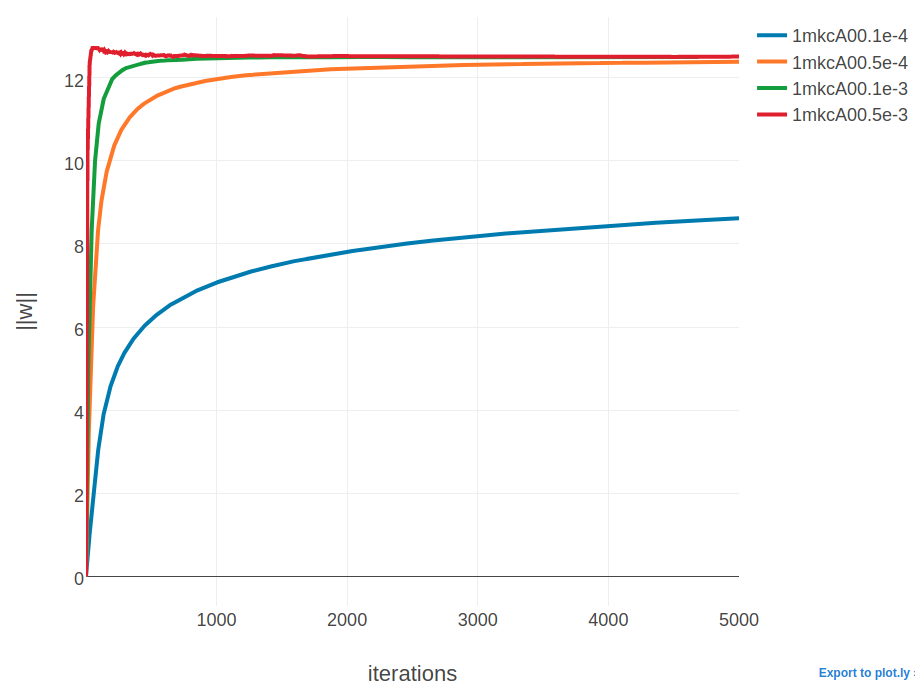
\includegraphics[width=0.5\linewidth]{img/full_likelihood/sgd/parameter_norm_1mkca00_alphas_lindecay001} 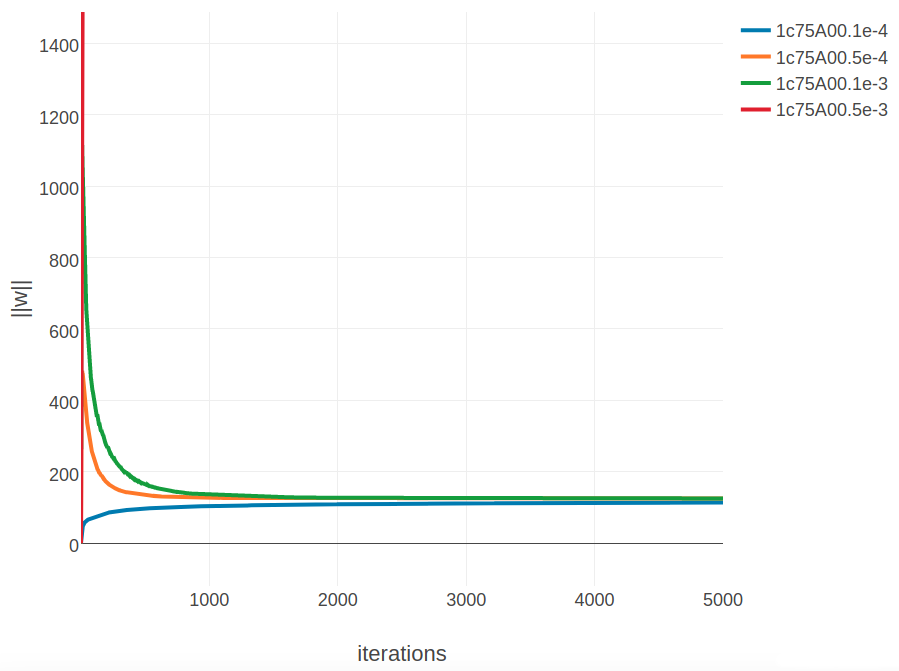
\includegraphics[width=0.5\linewidth]{img/full_likelihood/sgd/parameter_norm_1c75a00_alphas_lindecay001} 

}

\caption{L2-norm of the
coupling parameters \(||\w||_2\) during stochastic gradient descent
optimization with different learning rates. Linear learning rate
annealing schedule has been used with decay rate \(\gamma=0.01\) and
initial learning rates \(\alpha_0\) as stated in the legend.
\textbf{Left} Convergence plot for protein 1mkc\_A\_00 having protein
length L=43 and 142 sequences in the alignment
(\protect\hyperlink{abbrev}{Neff}=96). \textbf{Right} Convergence plot
for protein 1c75\_A\_00 having protein length L=71 and 28078 sequences
in the alignment (\protect\hyperlink{abbrev}{Neff}=16808). Figure is cut
at the yaxis at \(||\w||_2=1500\), but learning rate of
\(5\mathrm{e}{-3}\) reaches \(||\w||_2 \approx 13000\).}\label{fig:sgd-single-proteins-initial-learning-rate}
\end{figure}

In a next step, I tried to find an optimal learning rate annealing
schedule and an optimal decay rate. I evaluated the following learning
rate schedules and decay rates using the
\protect\hyperlink{abbrev}{Neff} dependent definition of the initial
learning given in eq. \eqref{eq:learning-rate-wrt-neff}:

\begin{itemize}
\tightlist
\item
  default linear learning rate schedule
  \(\alpha = \frac{\alpha_0}{1 + \gamma t}\) with
  \(\gamma \in \{1\mathrm{e}{-3}, 1\mathrm{e}{-2}, 1\mathrm{e}{-1}, 1 \}\)
\item
  square root learning rate schedule
  \(\alpha = \frac{\alpha_0}{\sqrt{1 + \gamma t}}\) with
  \(\gamma \in \{1\mathrm{e}{-2}, 1\mathrm{e}{-1}, 1 \}\)
\item
  sigmoidal learning rate schedule
  \(\alpha_{t+1} = \frac{\alpha_{t}}{1 + \gamma t}\) with
  \(\gamma \in \{1\mathrm{e}{-6}, 1\mathrm{e}{-5}, 1\mathrm{e}{-4}, 1\mathrm{e}{-3}\}\)
\item
  exponential learning rate schedule
  \(\alpha_{t+1} = \alpha_0 \cdot\exp(- \gamma t)\) with
  \(\gamma \in \{5\mathrm{e}{-4}, 1\mathrm{e}{-4}, 5\mathrm{e}{-3}\}\)
\end{itemize}

The different learning rate annealing schedules and decay rates are
visualized in Appendix Figure \ref{fig:learning-rate-schedules} and the
respective benchmark plots can be found in Appendix
\ref{benchmark-learning-rate-annealing-schedules}. None of the learning
rate schedules achieves an average precision for the top ranked contacts
that is comparable to the pseudo-likelihood score. The highest
precision, being one to two percentage points below the
pseudo-likelihood score, is obtained with a linear learning rate
schedule and decay rate \(\gamma \eq 1\mathrm{e}{-2}\) and with a
sigmoidal learning rate schedule and decay rates
\(\gamma \eq 1\mathrm{e}{-5}\) and \(\gamma \eq 1\mathrm{e}{-6}\). The
square root learning rate schedule gives ovarally bad results and does
not lead to convergence because the learning rate decays slowly at later
time steps. The exp decay rate TODOOOO.

In contrast to the findings regarding the initial learning rate earlier,
an optimal decay rate is independent of the alignment size. Figure
\ref{fig:sgd-single-proteins-learning-rate-schedule} shows convergence
plots for the same two exemplary proteins with small and big alignments
as in Figure \ref{fig:sgd-single-proteins-initial-learning-rate}. For
proteins with small \protect\hyperlink{abbrev}{Neff}, a quickly decaying
learning rate such as \(\gamma \eq 1\mathrm{e}{-1}\) with a linear
schedule or \(\gamma \eq 1\mathrm{e}{-4}\) with a sigmoidal schedule
guide the optimization closely to the presumed optimum at
\(||w||_2 \approx 12.5\), as can be seen in the left plot in Figure
\ref{fig:sgd-single-proteins-learning-rate-schedule}. Proteins with big
\protect\hyperlink{abbrev}{Neff} are generally stronger adversely
affected by quickly decaying learning rates and the optimum at
\(||w||_2 \approx 125\) is not reached before the learning rate
diminishes, effectively preventing further optimization progress.
Learning rates decaying less quickly, such as
\(\gamma \eq 1\mathrm{e}{-2}\) with a linear schedule or
\(\gamma \eq 1\mathrm{e}{-6}\) with a sigmoidal schedule, guide the
parameter estimates close to the expected optimum, both for proteins
with small and big \protect\hyperlink{abbrev}{Neff}.














\begin{figure}

{\centering 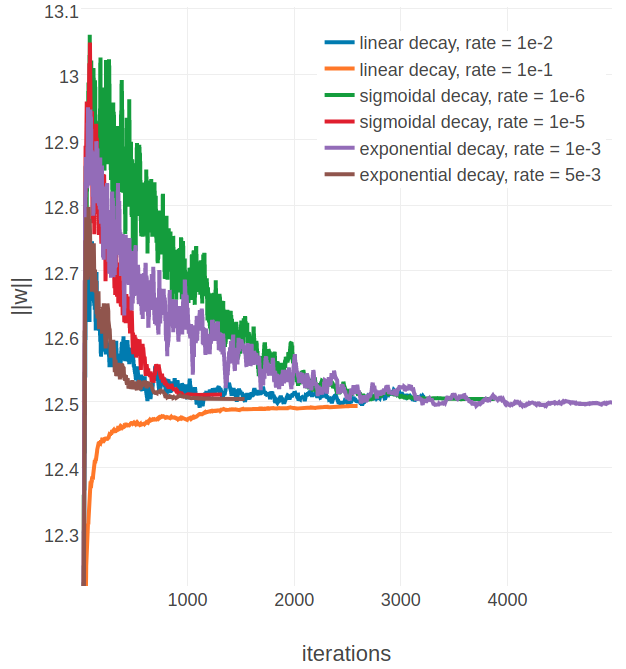
\includegraphics[width=0.5\linewidth]{img/full_likelihood/sgd/parameter_norm_1mkca00_alpha0_different_schedules} 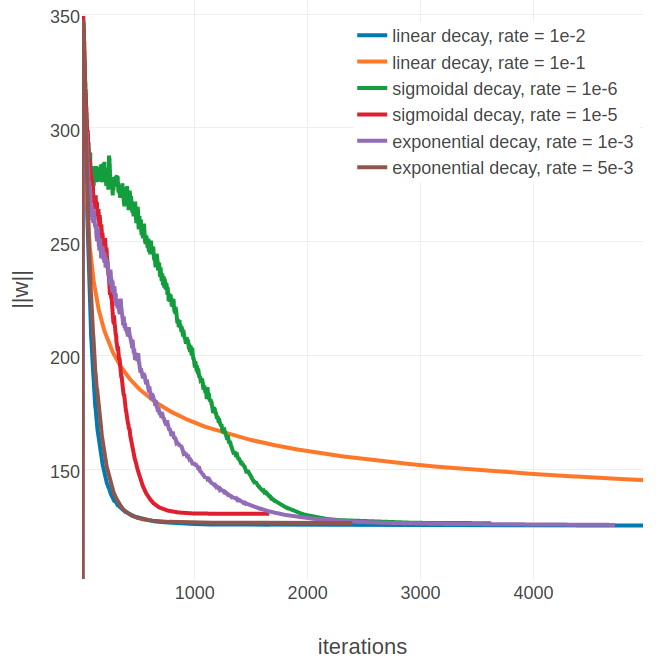
\includegraphics[width=0.5\linewidth]{img/full_likelihood/sgd/parameter_norm_1c75a00_alpha0_different_schedules} 

}

\caption{L2-norm of the
coupling parameters \(||\w||_2\) during stochastic gradient descent
optimization with different learning rates schedules. The initial
learning rate \(\alpha_0\) is defined with respect to
\protect\hyperlink{abbrev}{Neff} as given in eq.
\eqref{eq:learning-rate-wrt-neff}. Learning rate schedules and decay rates
are used according to the legend. \textbf{Left} Convergence plot for
protein 1mkc\_A\_00 having protein length L=43 and 142 sequences in the
alignment (\protect\hyperlink{abbrev}{Neff}=96). \textbf{Right}
Convergence plot for protein 1c75\_A\_00 having protein length L=71 and
28078 sequences in the alignment
(\protect\hyperlink{abbrev}{Neff}=16808).}\label{fig:sgd-single-proteins-learning-rate-schedule}
\end{figure}

While the three learning rate choices, linear learning rate schedule
with decay rate \(\gamma \eq 1\mathrm{e}{-2}\) and sigmoidal learning
rate schedule with decay rates \(\gamma \eq 1\mathrm{e}{-5}\) and
\(\gamma \eq 1\mathrm{e}{-6}\), give almost identical precision in the
benchmarks shown in Appendix
\ref{benchmark-learning-rate-annealing-schedules}, they differ in their
average rate until convergence. Figure
\ref{fig:distribution-num-iterations} shows the distribution over the
number of iterations until convergence for all three choices of learning
rate schedules. Optimization converges on average within 3584 iterations
with a sigmoidal schedule and \(\gamma \eq 1\mathrm{e}{-6}\) and within
1356 iterations when setting the decay rate
\(\gamma \eq 1\mathrm{e}{-5}\). On the contrary, when using a linear
learning rate schedule with \(\gamma \eq 1\mathrm{e}{-2}\), optimization
converges on average within 4276 iterations but the distribution has a
median of 5000. Under these considerations, I chose a sigmoidal learning
rate schedule with \(\gamma \eq 5\mathrm{e}{-6}\) for all further
analysis.












\begin{figure}

{\centering 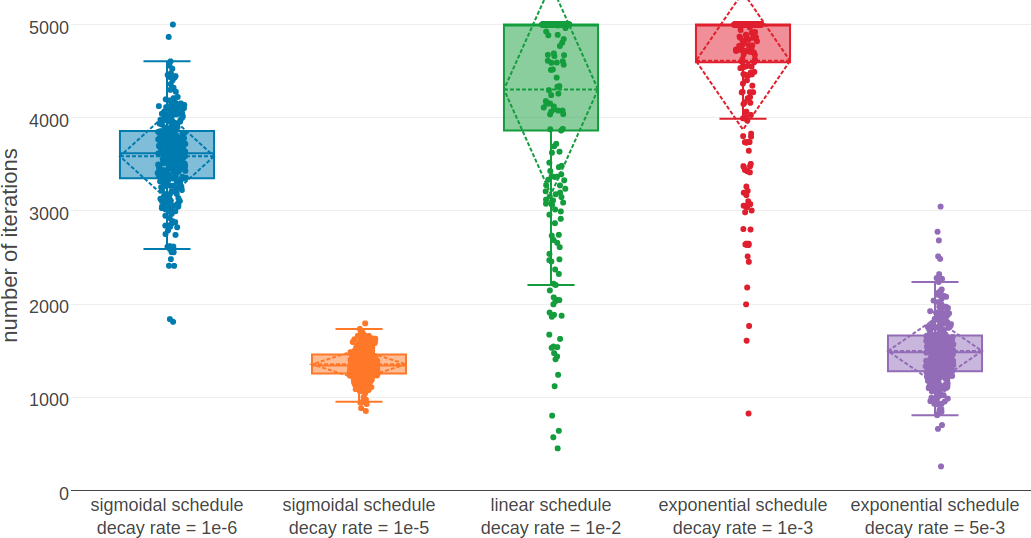
\includegraphics[width=1\linewidth]{img/full_likelihood/sgd/distribution_numiterations_against_selected_learningrate_schedules} 

}

\caption{Distribution of the number of
iterations until convergence for \protect\hyperlink{abbrev}{SGD}
optimizations of the full likelihood for different learning rate
schedules. Convergence is reached when the relative difference of
parameter norms \(||\w||_2\) falls below \(\epsilon \eq 1e-8\). Initial
learning rate \(\alpha_0\) is defined with respect to
\protect\hyperlink{abbrev}{Neff} as given in eq.
\eqref{eq:learning-rate-wrt-neff} and maximum number of iterations is set
to 5000. Learning rate schedules and decay rates are used according to
the legend.}\label{fig:distribution-num-iterations}
\end{figure}

\subsection{Optimizing Regularization Coefficients for Contrastive
Divergence}\label{optimizing-regularization-coefficients-for-contrastive-divergence}

Gaussian priors are put on the single potentials \(\v\) and the
couplings \(\w\) when optimizing the full likelihood with
\protect\hyperlink{abbrev}{CD} just as it is done for pseudo-likelihood
optimization (compare section \ref{pseudo-likelihood}). A difference
compared to pseudo-likelihood optimization that uses zero centered
priors, is the centering of the Gaussian prior for the single potentials
\(\v\) at \(v^*\) as described in section \ref{prior-v}. The
hyperparameter tuning for stochastic gradient descent described in the
last section applied the default pseudo-likelihood regularization
coefficients \(\lambda_v \eq 10\) and \(\lambda_w \eq 0.2\cdot(L-1)\).
The regularization coefficient \(\lambda_w\) for couplings \(\w\) is
defined with respect to protein length \(L\) owing to the fact that the
number of possible contacts in a protein increases quadratically with
\(L\) whereas the number of observed contacts only increases linearly as
can be seen in Figure \ref{fig:number-contacts-against-L}.





\begin{figure}

{\centering 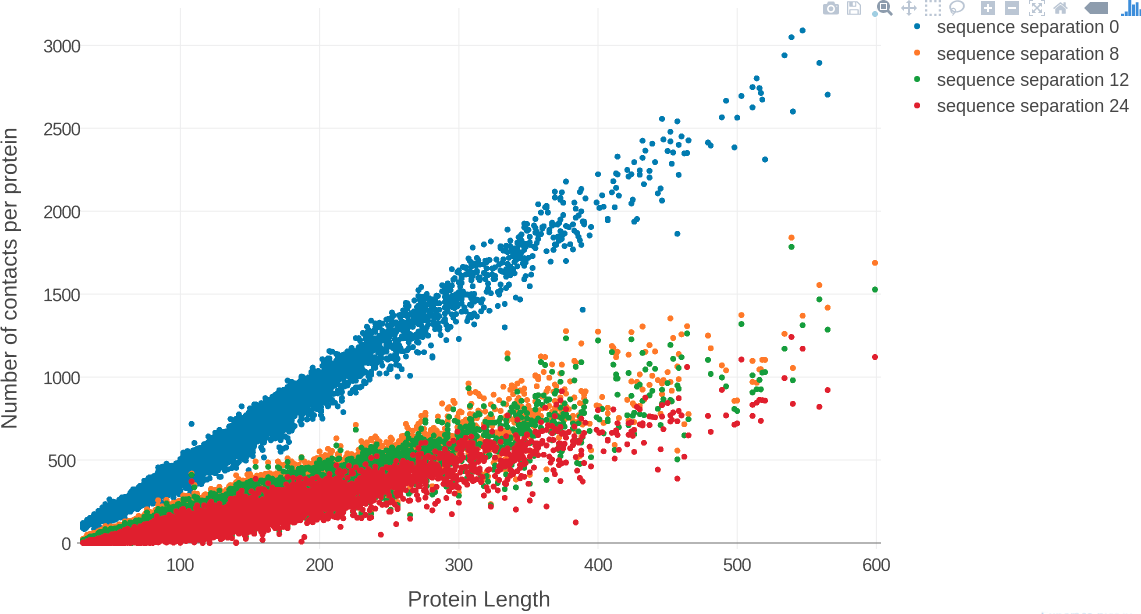
\includegraphics[width=0.9\linewidth]{img/full_likelihood/no_contacts_vs_protein_length_thr8} 

}

\caption{Number of contacts
(\(\Cb < 8 \angstrom\)) with respect to protein length and sequence
separation has a linear relationship.}\label{fig:number-contacts-against-L}
\end{figure}

It is possible that \protect\hyperlink{abbrev}{CD} achieves optimal
performance using stronger or weaker regularization coefficients
compared to pseudo-likelihood. Therefore, I evaluated performance of
contrastive divergence using different regularization coefficients
\(\lambda_w \in \{ 1\mathrm{e}{-2}, 1\mathrm{e}{-1}, 0.2, 1\} \cdot(L-1)\)
while leaving the regularization for single potentials at the default
value \(\lambda_v \eq 10\). Furthermore, I analysed whether precision is
impacted by only optimizing the couplings \(\w\) (with default
regularization) while fixing the single potentials \(\vi\) to their best
estimates \(\vi^*\) as described in section \ref{prior-v}.

As can be seen in Figure \ref{fig:precison-cd-regularization}, using
strong regularization for the couplings \(\lambda_w \eq (L-1)\) results
in a drop of mean precision. Using weaker regularization or fixing the
single potentials hardly has an impact on precision with using
\(\lambda_w \eq 1\mathrm{e}{-2}(L-1)\) yielding slightly improved
precision for the top ranked contacts.

















\begin{figure}

{\centering 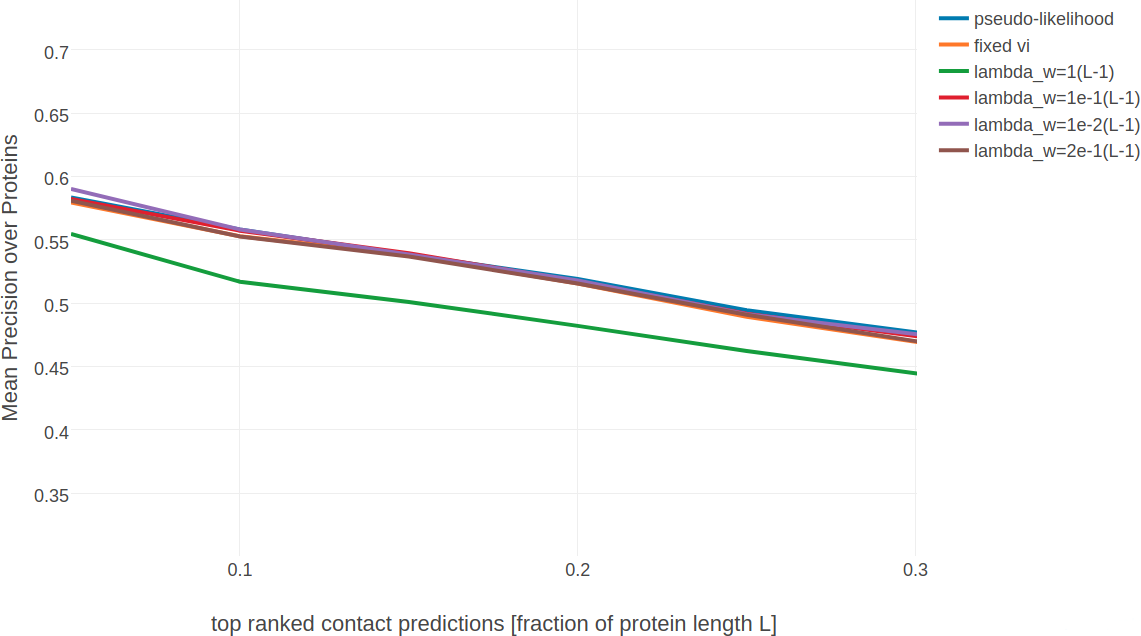
\includegraphics[width=0.9\linewidth]{img/full_likelihood/precision_vs_rank_notitle_cd_comparing_regularizers} 

}

\caption{Performance of contrastive
divergence optimization of the full likelihood with different
regularization settings compared to pseudo-likelihood (blue) for 280
proteins. Contact scores are computed as the
\protect\hyperlink{abbrev}{APC} corrected Frobenius norm of the
couplings \(\wij\). Default regularization coefficients as used with
pseudo-likelihood are \(\lambda_v \eq 10\) and
\(\lambda_w \eq 0.2(L-1)\). ``fixed vi'' (orange) uses
\protect\hyperlink{abbrev}{CD} to optimize only couplings with default
regularization while keeping the single potentials \(\vi\) fixed at
their \protect\hyperlink{abbrev}{MLE} optimum \(\vi^*\). The other
optimization runs with \protect\hyperlink{abbrev}{CD} (green, red,
purple, brown) use default regularization for the single potentials and
a regularization coefficient for the couplings according to legend
description.}\label{fig:precison-cd-regularization}
\end{figure}

\subsection{Optimizing the Sampling Scheme for Contrastive
Divergence}\label{optimizing-the-sampling-scheme-for-contrastive-divergence}

I analysed whether choosing a different number of sequences for the
approximation of the gradient via Gibbs sampling can improve
performance. Randomly selecting only a subset \(N^{\prime}\) of the
\(N\) observed sequences corresponds to the stochastic gradient descent
idea of a minibatch and introduces additional stochasticity over the
random Gibbs sampling process. Using \(N^{\prime} < N\) sequences for
Gibbs sampling has the further advantage of decreasing the runtime at
each iteration. Note, that the reference counts from the observed
sequences \(N_{ij} q(x_i \eq a, x_j \eq b)\) that are part of the
gradient calculation will be kept constant. Therefore it is necessary,
however to rescale the amino acid counts from the sampled sequences in a
way such that the total sample counts match the total observed counts.

I evaluated two different schemes for randomly selecting
\(N^{\prime} \eq xL\) sequences from the \(N\) given sequences of the
alignment at every iteration:

\begin{itemize}
\tightlist
\item
  \textbf{without} replacement (enforcing
  \(N^{\prime} \eq \min(N, xL)\))
\item
  \textbf{with} replacement
\end{itemize}

with \(x \in \{ 1, 5, 10, 50 \}\).

As can be seen in the Figure \ref{fig:cd-sampling-size}, the choice of
minibatch size which corresponds to the number sequences that are
selected to approximate the gradient, has no influence on precision.

PLOT PEFORMANCE SMAPLING SIZE

This results is somewhat unexpected, because using more samples to
approximate the gradient should result in a better gradient
approximation and thus in a better performance. Indeed, the magnitude of
the gradient norms decreases when more sequences are used for sampling
as can be seen in Figure \ref{fig:cd-gradient-norm}. However, this does
apparantly not translate into better parameter values.

PLOT GRADIENT NORMS

The default \protect\hyperlink{abbrev}{CD} algorithm as described by
Hinton in 2002 applies only one full step of Gibbs sampling on each data
sample to generate a sampled data set that will be used to approximate
the gradient {[}\protect\hyperlink{ref-Hinton2002}{32}{]}. One full step
of Gibbs sampling corresponds to sampling each position in a protein
sequence according to the conditional probabilities computed from the
current model probabilties as described in \ref{gibbs-sampling}. The
sampled sequences obtained after only one step of Gibbs sampling will be
very similar to the input sequences. It has been shown that sampling
with \(n>1\) steps gives more precise results but increases
computational cost per gradient evaluation
{[}\protect\hyperlink{ref-Bengio2009}{33},\protect\hyperlink{ref-Tieleman2008}{34}{]}.

In the following I analysed the impact on performance when Gibbs
sampling each sequence with 1, 5 and 10 full steps. As can be seen,
there is hardly an impact on precision while having much longer runtimes
(by a factor or 5 and 10).











\begin{figure}

{\centering 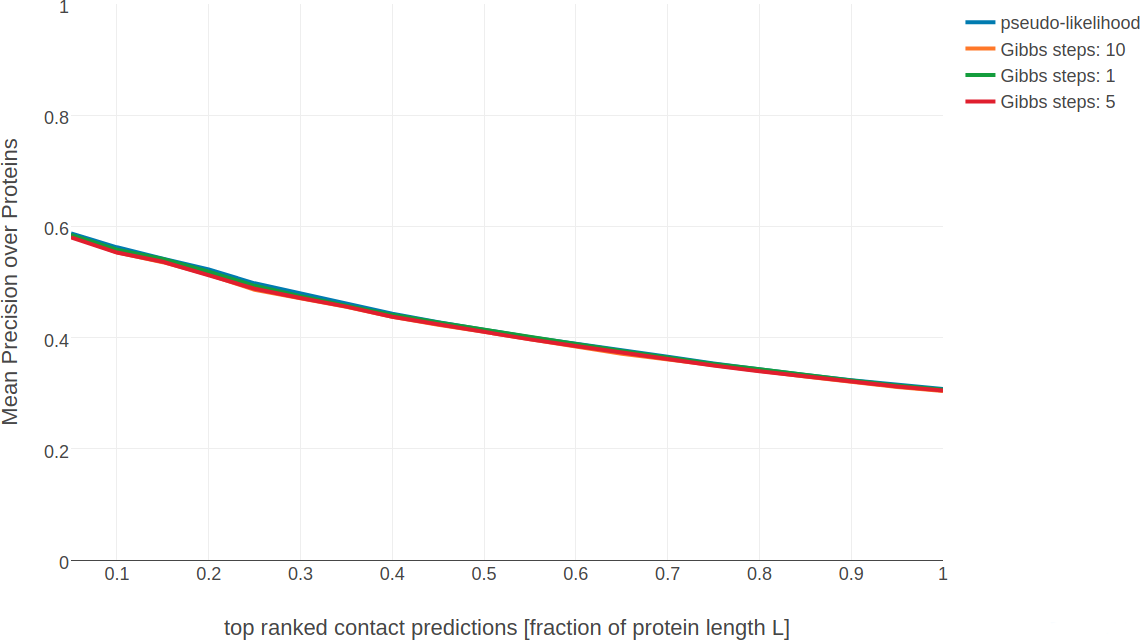
\includegraphics[width=0.9\linewidth]{img/full_likelihood/precision_vs_rank_notitle_cd_comparing_nr_of_gibbs_sampling_steps} 

}

\caption{Performance of contrastive
divergence optimization of the full likelihood with different number of
Gibbs steps compared to pseudo-likelihood (blue) for 287 proteins.
Contact scores are computed as the \protect\hyperlink{abbrev}{APC}
corrected Frobenius norm of the couplings \(\wij\). pseudo-likelihood:
contact scores computed from pseudo-likelihood. The other methods derive
contact scores from couplings computed from
\protect\hyperlink{abbrev}{CD} with different number of Gibbs sampling
steps.}\label{fig:precision-cd-gibbs-steps}
\end{figure}

Another variant of \protect\hyperlink{abbrev}{CD} that has been
suggested by Tieleman in 2008 is
\protect\hyperlink{abbrev}{\emph{PCD}}{[}\protect\hyperlink{ref-Tieleman2008}{34}{]}
that does not reset the Markov Chains at every iteration. The reason
being that when using small learning rates, the model changes only
slightly between iterations and the true data distribution can be better
approximated However, subsequent samples of
\protect\hyperlink{abbrev}{\emph{PCD}} will be highly correlated
creating a kind of momentum effect. Furthermore is has been found that
\protect\hyperlink{abbrev}{\emph{PCD}} should be used with smaller
learning rates and higher minibatch sizes.

As PCD might require samller update steps and larger minibatches, I
analysed the performance of PCD for the default settings of CD and
additionally for smaller learning and decay rates and larger
minibatches. Note that one Markov chain is kept for every sequence of
the input alignment. At each iteration a subset \(N^{\prime} < N\) of
the Markov chains is randomly selected (without replacement) and used to
for another round of Gibss sampling at the current iteration.

PLOT PCD for different LEARNIGN RATEWS and SAMPLE SIZES

\section{Bayesian Model for Residue-Resdiue Contact
Prediction}\label{bayesian-model-for-residue-resdiue-contact-prediction}

\subsection{Efficiently Computing the negative Hessian of the
regularized log-likelihood}\label{neg-Hessian-computation}

Surprisingly, the elements of the Hessian at the mode \(\w^*\) are easy
to compute. Let \(i,j,k,l \in \{1,\ldots,L\}\) be columns in the
\protect\hyperlink{abbrev}{MSA} and let
\(a, b, c, d \in \{1,\ldots,20\}\) represent amino acids.

The partial derivative \(\partial / \partial \w_{klcd}\) of the second
term in the gradient of the couplings in eq.
\eqref{eq:gradient-LLreg-pair} is

\begin{eqnarray}
    \frac{\partial^2 \LLreg(\v^*,\w)}{\partial \wklcd \, \partial \wijab } 
    &=&  - \sum_{n=1}^{N} \, \sum_{\mathbf{y} \in \Sn} \frac{\partial \left( \frac{\exp \left( \sum_{i=1}^L v_i(y_i) + \sum_{1 \le i < j \le L}^L w_{ij}(y_i,y_j) \right) }{Z_n(\v,\w)} \right)}{\partial \wklcd}   I(y_i \eq a, y_j \eq b) \\
    &&- \lambda_w \delta_{ijab,klcd} \,,
\end{eqnarray}

where \(\delta_{ijab,klcd} = I(ijab=klcd)\) is the Kronecker delta.
Applying the product rule, we find

\begin{eqnarray}
    \frac{\partial^2 \LLreg(\v^*,\w)}{\partial \wklcd \, \partial \wijab  } 
    &=&  - \sum_{n=1}^{N} \, \sum_{\mathbf{y} \in \Sn} \frac{\exp \left(\sum_{i=1}^L v_i(y_i) + \sum_{1 \le i < j \le L}^L w_{ij}(y_i,y_j)  \right)}{Z_n(\v,\w)}  I(y_i \eq a, y_j \eq b) \\
    & \times & \left[ \frac{\partial}{\partial \wklcd} \left( \sum_{i=1}^L v_i(y_i) + \sum_{1 \le i < j \le L}  w_{ij}(y_i,y_j)  \right) 
                  - \frac{1}{Z_n(\v,\w)} \frac{\partial  Z_n(\v,\w) }{\partial\wklcd} \right] \\
    &-& \lambda_w \delta_{ijab,klcd} \\
    \frac{\partial^2 \LLreg(\v^*,\w)}{\partial \wklcd \, \partial \wijab  } 
    &=&  - \sum_{n=1}^{N} \, \sum_{\mathbf{y} \in \Sn} \frac{\exp \left(\sum_{i=1}^L v_i(y_i) + \sum_{1 \le i < j \le L}^L w_{ij}(y_i,y_j)  \right)}{Z_n(\v,\w)}  I(y_i \eq a, y_j \eq b) \\
    & \times & \left[ I(y_k \eq c, y_l \eq d) - \frac{\partial}{\partial \wklcd} \log Z_n(\v,\w) \right] \\
    &-& \lambda_w \delta_{ijab,klcd} \,.
\end{eqnarray}

We simplify this expression using

\begin{equation}
    p(\mathbf{y} | \v,\w) = \frac{\exp \left( \sum_{i=1}^L v_i(y_i) + \sum_{1 \le i < j \le L} w_{ij}(y_i,y_j) \right)}{Z_n(\v,\w)}  ,
\end{equation}

yielding

\begin{eqnarray}
    \frac{\partial^2 \LLreg(\v^*,\w)}{\partial \wklcd \, \partial \wijab} 
    &=&  -  \sum_{n=1}^{N} \, \sum_{\mathbf{y} \in \Sn} p(\mathbf{y} | \v,\w) \, I(y_i \eq a, y_j \eq b, y_k \eq c, y_l \eq d)  \\
    &+& \sum_{n=1}^{N} \, \sum_{\mathbf{y} \in \mathcal{S}_n} p(\mathbf{y} | \v,\w) \, I(y_i \eq a, y_j \eq b ) \sum_{\mathbf{y} \in \Sn} p(\mathbf{y} | \v,\w)  I(y_k \eq c, y_l \eq d ) \\
    &-& \lambda_w \delta_{ijab,klcd} \,.
\end{eqnarray}

If \(\X\) does not contain too many gaps, this expression can be
approximated by

\begin{eqnarray}
    \frac{\partial^2 \LLreg(\v^*,\w)}{\partial \wklcd \, \partial \wijab  } 
    &=& - N_{ijkl} \: p(x_i \eq a, x_j \eq b, x_k \eq c, x_l \eq d | \v,\w)  \nonumber \\
    && +  N_{ijkl} \: p(x_i \eq a, x_j \eq b | \v,\w) \, p(x_k \eq c, x_l \eq d | \v,\w) - \lambda_w \delta_{ijab,klcd} \,,
\end{eqnarray}

where \(N_{ijkl}\) is the number of sequences that have a residue in
\(i\), \(j\), \(k\) and \(l\).

Looking at three cases separately:

\begin{itemize}
\tightlist
\item
  case 1: \((k,l) = (i,j)\) and \((c,d) = (a,b)\)
\item
  case 2: \((k,l) = (i,j)\) and \((c,d) \ne (a,b)\)
\item
  case 3: \((k,l) \ne (i,j)\) and \((c,d) \ne (a,b)\),
\end{itemize}

the elements of \(\H\), which are the negative second partial
derivatives of \(\LLreg(\v^*,\w)\) with respect to the components of
\(\w\), are

\begin{eqnarray}
    \mathrm{case~1:} (\H)_{ijab, ijab}  
    &=&  N_{ij} \, p(x_i \eq a, x_j \eq b| \v^*,\w^*) \, ( 1 - p(x_i \eq a, x_j \eq b| \v^*,\w^*) \,) \\
    &&   + \lambda_w \\
    \mathrm{case~2:} (\H)_{ijcd, ijab}  
    &=&  - N_{ij} \, p(x_i \eq a, x_j \eq b |\v^*,\w^*) \, p(x_i \eq c, x_j \eq d |\v^*,\w^*) \\
    \mathrm{case~3:} (\H)_{klcd, ijab}  
    &=&   N_{ijkl} \, p(x_i \eq a, x_j \eq b, x_k \eq c, x_l \eq d  | \v^*,\w^*) \nonumber \\
    &&    - N_{ijkl} \, p(x_i \eq a, x_j \eq b | \v^*,\w^*)\, p(x_k \eq c, x_l \eq d | \v^*,\w^*) \,.
\label{eq:Hw-offdiag}
\end{eqnarray}

We know from eq. \eqref{eq:gradient-LLreg-approx} that at the mode
\(\w^*\) the model probabilities match the empirical frequencies up to a
small regularization term,

\begin{equation}
    p(x_i \eq a, x_j \eq b | \v^*,\w^*) = q(x_i \eq a, x_j \eq b) - \frac{\lambda_w}{N_{ij}}  \wijab^* \,,
\end{equation}

and therefore the negative Hessian elements in cases 1 and 2 can be
expressed as

\begin{align}
   (\H)_{ijab, ijab} =& N_{ij} \left( q(x_i \eq a, x_j \eq b)  - \frac{\lambda_w}{N_{ij}} \wijab^* \right) \left( 1 - q(x_i \eq a, x_j \eq b) +\frac{\lambda_w}{N_{ij}} \wijab^* \right) \\
   & + \lambda_w \\
   (\H)_{ijcd, ijab} =& -N_{ij} \left(\,q(x_i \eq a, x_j \eq b)  - \frac{\lambda_w}{N_{ij}} \wijab^* \right) \left( q(x_i \eq c, x_j \eq d) -\frac{\lambda_w}{N_{ij}} \wijcd^* \right) .
\label{eq:Hw-diag}
\end{align}

In order to write the previous eq. \eqref{eq:Hw-diag} in matrix form, the
\emph{regularised} empirical frequencies \(\qij\) will be defined as

\begin{equation}
    (\qij)_{ab} = q'_{ijab} := q(x_i \eq a, x_j \eq b) - \lambda_w  \wijab^* / N_{ij} \,,
\end{equation}

and the \(400 \times 400\) diagonal matrix \(\Qij\) will be defined as

\begin{equation}
    \Qij := \text{diag}(\qij) \; .
\end{equation}

Now eq. \eqref{eq:Hw-diag} can be written in matrix form

\begin{equation}
     \H_{ij} = N_{ij} \left( \Qij -  \qij \qij^{\mathrm{T}} \right)  + \lambda_w \I \; .
\label{eq:mat-Hij}
\end{equation}

\subsection{\texorpdfstring{Efficiently Computing the Inverse of Matrix
\(\Lijk\)}{Efficiently Computing the Inverse of Matrix \textbackslash{}Lijk}}\label{inv-lambda-ij-k}

It is possible to efficiently invert the matrix
\(\Lijk = \H_{ij} - \lambda_w \I + \Lambda_k\), that is introduced in
\ref{coupling-prior} where \(\H_{ij}\) is the \(400 \times 400\)
diagonal block submatrix \((\H_{ij})_{ab,cd} := (\H)_{ijab,ijcd}\) and
\(\Lambda_k\) is an invertible diagonal precision matrix that is
introduced in section \ref{modeling-dep-of-wij}.

Equation \eqref{eq:mat-Hij} can be used to write \(\Lijk\) in matrix form
as

\begin{equation}
     \Lijk = \H_{ij} - \lambda_w \I + \Lk = N_{ij} \Qij- N_{ij} \qij \qij^{\mathrm{T}} + \Lk \,.
\label{eq:mat-Lijk}
\end{equation}

Owing to eqs. \eqref{eq:normalized-emp-freq} and \eqref{eq:zero-sum-wij},
\(\sum_{a,b=1}^{20} q'_{ijab} = 1\). The previous equation
\eqref{eq:mat-Lijk} facilitates the calculation of the inverse of this
matrix using the \emph{Woodbury identity} for matrices

\begin{equation}
    (\mathbf{A} + \mathbf{B} \mathbf{D}^{-1} \mathbf{C})^{-1} = \mathbf{A}^{-1} - \mathbf{A}^{-1} \mathbf{B} (\mathbf{D} + \mathbf{C} \mathbf{A}^{-1} \mathbf{B}) ^{-1} \mathbf{C} \mathbf{A}^{-1} \;. 
\end{equation}

by setting

\begin{align}
  \mathbf{A} &= N_{ij} \Qij + \Lk \\
  \mathbf{B} &= \qij \\
  \mathbf{C} &= \qij^\mathrm{T} \\
  \mathbf{D} &=- N_{ij}^{-1} \\
\end{align}

\begin{align}
      \left( \H_{ij} - \lambda_w \I + \Lk \right)^{-1} & = \mathbf{A}^{-1} - \mathbf{A}^{-1} \qij  \left( -N_{ij}^{-1}  + \qij^\mathrm{T} \mathbf{A}^{-1} \qij \right)^{-1}  \qij^\mathrm{T} \mathbf{A}^{-1} \\
     & = \mathbf{A}^{-1} + \frac{ (\mathbf{A}^{-1} \qij) (\mathbf{A}^{-1} \qij)^{\mathrm{T}} }{ N_{ij}^{-1} - \qij^\mathrm{T} \mathbf{A}^{-1} \qij} \,.
\label{eq:fast-inverse-mat-Lijk}
\end{align}

Note that \(\mathbf{A}\) is diagonal as \(\Qij\) and \(\Lk\) are
diagonal matrices:
\(\mathbf{A} = \text{diag}(N_{ij} q'_{ijab} + (\Lk)_{ab,ab})\).
Moreover, \(\mathbf{A}\) has only positive diagonal elements, because
\(\Lk\) is invertible and has only positive diagonal elements and
because \(q'_{ijab} = p(x_i \eq a, x_j \eq b | \v^*,\w^*) \ge 0\).

Therefore \(\mathbf{A}\) is invertible:
\(\mathbf{A}^{-1} = \text{diag}(N_{ij} q'_{ijab} + (\Lk)_{ab,ab} )^{-1}\).

Because \(\sum_{a,b=1}^{20} q'_{ijab} = 1\), the denominator of the
second term is

\begin{equation}
    N_{ij}^{-1} - \sum_{a,b=1}^{20}  \frac{{q'}_{ijab}^2}{N_{ij} q'_{ijab} + {(\Lk)}_{ab,ab} } > N_{ij}^{-1} - \sum_{a,b=1}^{20} \frac{{q'}^2_{ijab}}{N_{ij} q'_{ijab}} = 0
\end{equation}

and therefore the inverse of \(\Lijk\) in eq.
\eqref{eq:fast-inverse-mat-Lijk} is well defined.

The log determinant of \(\Lijk\) is necessary to compute the ratio of
Gaussians (see equation \eqref{eq:p-X-r-final}) and can be computed using
the matrix determinant lemma:

\begin{equation}
  \det(\mathbf{A} + \mathbf{uv}^\mathrm{T}) = (1+\mathbf{v}^\mathrm{T} \mathbf{A}^{-1} \mathbf{u}) \det(\mathbf{A})
\end{equation}

Setting \(\mathbf{A} = N_{ij} \Qij + \Lk\) and \(\v = \qij\) and
\(\mathbf{u} = - N_{ij} \qij\) yields

\begin{equation}
  \det(\Lijk ) = \det(\H_{ij} - \lambda_w \I + \Lk) = (1 - N_{ij}\qij^\mathrm{T} \mathbf{A}^{-1}\qij) \det(\mathbf{A}) \,.
\end{equation}

\(\mathbf{A}\) is diagonal and has only positive diagonal elements so
that
\(\log(\det(\mathbf{A})) = \sum \log \left( \text{diag}(\mathbf{A}) \right)\).

\subsection{\texorpdfstring{Training the Hyperparameters \(\muk\),
\(\Lk\) and
\(\gamma_k\)}{Training the Hyperparameters \textbackslash{}muk, \textbackslash{}Lk and \textbackslash{}gamma\_k}}\label{training-hyperparameters}

The model parameters
\(\mathbf{\mu} = (\mathbf{\mu}_{1},\ldots,\mathbf{\mu}_K)\),
\(\mathbf{\Lambda} = (\mathbf{\Lambda}_1,\ldots,\mathbf{\Lambda}_K)\)
and \(\mathbf{\gamma} = (\mathbf{\gamma}_1,\ldots,\mathbf{\gamma}_K)\)
will be trained by maximizing the logarithm of the full likelihood over
a set of training \protect\hyperlink{abbrev}{MSAs} \(\X^1,\ldots,\X^N\)
and associated structures with distance vectors \(\r^1,\ldots,\r^N\)
plus a regularizer \(R(\mathbf{\mu}, \mathbf{\Lambda})\):

\begin{equation}
    L\!L(\mathbf{\mu}, \mathbf{\Lambda}, \mathbf{\gamma}) + R(\mathbf{\mu}, \mathbf{\Lambda}) = \sum_{n=1}^N  \log p(\X^n | \r^n, \mathbf{\mu}, \mathbf{\Lambda}, \mathbf{\gamma} ) + R(\mathbf{\mu}, \mathbf{\Lambda})  \rightarrow \max \, .
\end{equation}

The regulariser penalizes values of \(\muk\) and \(\Lk\) that deviate
too far from zero:

\begin{align}
    R(\mathbf{\mu}, \mathbf{\Lambda}) = -\frac{1}{2 \sigma_{\mu}^2} \sum_{k=1}^K \sum_{ab=1}^{400} \mu_{k,ab}^2 
                        -\frac{1}{2 \sigma_\text{diag}^2} \sum_{k=1}^K \sum_{ab=1}^{400} \Lambda_{k,ab,ab}^2
\label{eq:reg}
\end{align}

Reasonable values are \(\sigma_{\mu}=0.1\),
\(\sigma_\text{diag} = 100\).

The log likelihood can be optimized using LBFG-S-B{[}{\textbf{???}}{]},
which requires the computation of the gradient of the log likelihood.
For simplicity of notation, the following calculations consider the
contribution of the log likelihood for just one protein, which allows to
drop the index \(n\) in \(\rij^n\), \((\wij^n)^*\) and \(\Hij^n\).

From eq. \eqref{eq:pXr-final} the log likelihood for a single protein is

\begin{equation}
    L\!L(\mathbf{\mu}, \mathbf{\Lambda}, \gamma_k) =  \sum_{1 \le i < j \le L}  \log \sum_{k=0}^K g_{k}(\rij) \frac{\Gauss( \mathbf{0} | \muk, \Lk^{-1})}{\Gauss(\mathbf{0} | \muijk, \Lijk^{-1})}  + R(\mathbf{\mu}, \mathbf{\Lambda}) + \text{const.}\,.
\label{eq:ll-coupling-prior}
\end{equation}

\subsection{\texorpdfstring{The gradient of the log likelihood with
respect to
\(\mathbf{\mu}\)}{The gradient of the log likelihood with respect to \textbackslash{}mathbf\{\textbackslash{}mu\}}}\label{the-gradient-of-the-log-likelihood-with-respect-to-mathbfmu}

By applying the formula \(d f(x) / dx = f(x) \, d \log f(x) / dx\) to
compute the gradient of eq. \eqref{eq:ll-coupling-prior} (neglecting the
regularization term) with respect to \(\mu_{k,ab}\), one obtains

\begin{equation}
 \frac{\partial}{\partial \mu_{k,ab}} L\!L(\mathbf{\mu}, \mathbf{\Lambda}, \gamma_k)
    = \sum_{1\le i<j\le L}  
    \frac{ 
        g_{k}(\rij) \frac{  \Gauss ( \mathbf{0} | \muk, \Lk^{-1})}{\Gauss( \mathbf{0} | \muijk, \Lijk^{-1})} 
             \frac{\partial}{\partial \mu_{k,ab}}  \log \left( \frac{ \Gauss(\mathbf{0} | \muk, \Lk^{-1})}{\Gauss( \mathbf{0} | \muijk, \Lijk^{-1})} \right)  
     } { \sum_{k'=0}^K g_{k'}(\rij) \, \frac{ \Gauss(\mathbf{0} | \muk', \Lk'^{-1})}{\Gauss( \mathbf{0} | \muijk, \Lijk^{-1})}  } .
\label{eq:gradient-mukab}
\end{equation}

To simplify this expression, we define the responsibility of component
\(k\) for the posterior distribution of \(\wij\), the probability that
\(\wij\) has been generated by component \(k\):

\begin{align}
      p(k|ij)  = 
      \frac{ g_{k}(\rij) \frac{ \Gauss( \mathbf{0} | \muk, \Lk^{-1})}{\Gauss(\mathbf{0} | \muijk, \Lijk^{-1})} } 
    {\sum_{k'=0}^K g_{k'}(\rij) \frac{ \Gauss(\mathbf{0} | \muk', \Lk'^{-1})}{\Gauss( \mathbf{0} | \muijk', \Lijk'^{-1})} }  \,.
\label{eq:responsibilities}
\end{align}

By substituting the definition for responsibility,
\eqref{eq:gradient-mukab} simplifies

\begin{equation}
  \frac{\partial}{\partial \mu_{k,ab}}  L\!L(\mathbf{\mu}, \mathbf{\Lambda}, \gamma_k)
    = \sum_{1\le i<j\le L}  p(k | ij)  \frac{\partial}{\partial \mu_{k,ab}} \log \left( \frac{ \Gauss(\mathbf{0} | \muk, \Lk^{-1})}{\Gauss( \mathbf{0} | \muijk, \Lijk^{-1})} \right) ,
\label{eq:gradient-LL-mukab}
\end{equation}

and analogously for partial derivatives with respect to
\(\Lambda_{k,ab,cd}\).

The partial derivative inside the sum can be written

\begin{equation}
     \frac{\partial}{\partial \mu_{k,ab}} \log \left( \frac{ \Gauss(\mathbf{0} | \muk, \Lk^{-1})}{\Gauss( \mathbf{0} | \muijk, \Lijk^{-1})} \right)
    = \frac{1}{2}  \frac{\partial}{\partial \mu_{k,ab}}   \left( \log | \Lk | - \muk^\mathrm{T} \Lk \muk - \log | \Lijk | + \muijk^\mathrm{T} \Lijk \muijk \right)\,.
\end{equation}

Using the following formula for a matrix \(\mathbf{A}\), a real variable
\(x\) and a vector \(\mathbf{y}\) that depends on \(x\),

\begin{equation}
    \frac{\partial}{\partial x} \left( \mathbf{y}^\mathrm{T} \mathbf{A} \mathbf{y} \right) = \frac{\partial \mathbf{y}^\mathrm{T}}{\partial x}  \mathbf{A} \mathbf{y} + \mathbf{y}^\mathrm{T} \mathbf{A} \frac{\partial \mathbf{y}}{\partial x}  =  \mathbf{y}^\mathrm{T} (\mathbf{A} + \mathbf{A}^\mathrm{T}) \frac{\partial \mathbf{y}}{\partial x} 
\label{eq:matrix-gradient}
\end{equation}

the partial derivative therefore becomes

\begin{align}
     \frac{\partial}{\partial \mu_{k,ab}} \log \left( \frac{ \Gauss(\mathbf{0} | \muk, \Lk^{-1})}{\Gauss( \mathbf{0} | \muijk, \Lijk^{-1})} \right)
    =& \left( -\muk^\mathrm{T} \Lk \mathbf{e}_{ab} \, +  \muijk^\mathrm{T} \Lijk \Lijk^{-1} \Lk \mathbf{e}_{ab} \right) \\
    =& \mathbf{e}^\mathrm{T}_{ab} \Lk ( \muijk - \muk ) \; . 
\end{align}

Finally, the gradient of the log likelihood with respect to
\(\mathbf{\mu}\) becomes

\begin{align}
    \nabla_{\muk} L\!L(\mathbf{\mu}, \mathbf{\Lambda}, \gamma_k)
    =  \sum_{1\le i<j\le L}  p(k|ij)  \,  \Lk \left(  \muijk  - \muk \right) \; .
\label{eq:gradient-muk-final}
\end{align}

\subsection{\texorpdfstring{The gradient of the log likelihood with
respect to
\(\Lk\)}{The gradient of the log likelihood with respect to \textbackslash{}Lk}}\label{the-gradient-of-the-log-likelihood-with-respect-to-lk}

Analogously to eq. \eqref{eq:gradient-LL-mukab} one first needs to solve

\begin{align}
     & \frac{\partial}{\partial \Lambda_{k,ab,cd}} \log \frac{\Gauss( \mathbf{0} | \muk, \Lk^{-1})}{\Gauss( \mathbf{0} | \muijk, \Lijk^{-1})} 
    = \\
    &\frac{1}{2}  \frac{\partial}{\partial \Lambda_{k,ab,cd}}  \left( \log |\Lk| - \muk^\mathrm{T} \Lk \muk - \log |\Lijk| + \muijk^\mathrm{T} \Lijk \muijk \right) \,,
\label{eq:grad-log-N-N-lambdakabcd}
\end{align}

by applying eq. \eqref{eq:matrix-gradient} as before as well as the
formulas

\begin{align}
    \frac{\partial}{\partial x} \log |\mathbf{A} | &= \text{Tr}\left( \mathbf{A}^{-1} \frac{\partial \mathbf{A}}{\partial x}  \right) , \\
    \frac{\partial \mathbf{A}^{-1}}{\partial x} &= - \mathbf{A}^{-1} \frac{\partial \mathbf{A}}{\partial x} \mathbf{A}^{-1} \,.
\end{align}

This yields

\begin{align}
\frac{\partial}{\partial \Lambda_{k,ab,cd}}  \log |\Lk|
     &= \text{Tr} \left( \Lk^{-1} \frac{\partial \Lk}{\partial \Lambda_{k,ab,cd}} \right) 
     = \text{Tr} \left( \Lk^{-1} \mathbf{e}_{ab} \mathbf{e}_{cd}^\mathrm{T} \right) 
     = \Lambda^{-1}_{k,cd,ab} \\
\frac{\partial}{\partial \Lambda_{k,ab,cd}}  \log |\Lijk|
     &= \text{Tr} \left( \Lijk^{-1} \frac{\partial (\H_{ij} - \lambda_w \I + \Lk)}{\partial \Lambda_{k,ab,cd}}   \right) 
     = \Lambda^{-1}_{ij,k,cd,ab} \\
\frac{\partial (\muk^\mathrm{T} \Lk \muk)}{\partial \Lambda_{k,ab,cd}} 
    &= \muk^\mathrm{T} \mathbf{e}_{ab} \mathbf{e}_{cd}^\mathrm{T} \muk 
    = \mathbf{e}_{ab}^\mathrm{T} \muk \muk^\mathrm{T} \mathbf{e}_{cd} = (\muk \muk^\mathrm{T})_{ab,cd} \\
\frac{\partial ( \muijk^\mathrm{T} \Lijk \muijk) }{\partial \Lambda_{k,ab,cd}} 
    &= \muijk^\mathrm{T} \frac{\partial \Lijk}{\partial \Lambda_{k,ab,cd}} \muijk 
    + 2 \muijk^\mathrm{T} \Lijk \frac{\partial \Lijk^{-1}}{\partial \Lambda_{k,ab,cd}}  (\Hij \wij^* + \Lk \muk) 
    + 2 \muijk^\mathrm{T} \frac{\partial \Lk}{\partial \Lambda_{k,ab,cd}} \muk \nonumber \\
    &= (\muijk \muijk^\mathrm{T} + 2 \muijk \muk^\mathrm{T})_{ab,cd} 
    - 2 \muijk^\mathrm{T} \Lijk  \Lijk^{-1} \frac{\partial \Lijk}{\partial \Lambda_{k,ab,cd}} \Lijk^{-1} (\Hij\wij^* + \Lk \muk) \\
    &= (\muijk \muijk^\mathrm{T} + 2 \muijk \muk^\mathrm{T})_{ab,cd} 
    - 2 \muijk^\mathrm{T}  \frac{\partial \Lijk}{\partial \Lambda_{k,ab,cd}} \muijk\\
    &= (- \muijk \muijk^\mathrm{T} + 2 \muijk \muk^\mathrm{T})_{ab,cd} \,.
\end{align}

Inserting these results into eq. \eqref{eq:grad-log-N-N-lambdakabcd}
yields

\begin{align}
     \frac{\partial}{\partial \Lambda_{k,ab,cd}} \log \frac{  \Gauss(\mathbf{0} | \muk, \Lk^{-1})}{\Gauss( \mathbf{0} | \muijk, \Lijk^{-1})} 
    = \frac{1}{2} \left( \Lk^{-1} - \Lijk^{-1} - (\muijk - \muk) (\muijk - \muk)^\mathrm{T} \right)_{ab,cd}\,.
\end{align}

Substituting this expression into the equation
\eqref{eq:gradient-LL-mukab} analogous to the derivation of gradient for
\(\mu_{k,ab}\) yields the equation

\begin{align}
    \nabla_{\Lk}  L\!L(\mathbf{\mu}, \mathbf{\Lambda}, \gamma_k)
    =  \frac{1}{2} \sum_{1\le i<j\le L}  p(k|ij)  \, 
        \left( \Lk^{-1} - \Lijk^{-1} - (\muijk - \muk) (\muijk - \muk)^\mathrm{T} \right). 
\label{eq:gradient-lambdak-final}
\end{align}

\subsection{\texorpdfstring{The gradient of the log likelihood with
respect to
\(\gamma_k\)}{The gradient of the log likelihood with respect to \textbackslash{}gamma\_k}}\label{the-gradient-of-the-log-likelihood-with-respect-to-gamma_k}

With \(\rij \in \{0,1\}\) defining a residue pair in physical contact or
not in contact, the mixing weights can be modelled as a softmax function
according to eq. \eqref{eq:def-g-k-binary}. The derivative of the mixing
weights \(g_k(\rij)\) is:

\begin{eqnarray}
\frac{\partial g_{k'}(\rij)} {\partial \gamma_k} = \left\{
  \begin{array}{lr}
    g_k(\rij) (1 - g_k(\rij)) & : k' = k\\
    g_{k'}(\rij) - g_k(\rij)  & : k' \neq k
  \end{array}
  \right.
\end{eqnarray}

The partial derivative of the likelihood function with respect to
\(\gamma_k\) is:

\begin{align}
\frac{\partial} {\partial \gamma_k}     L\!L(\mathbf{\mu}, \mathbf{\Lambda}, \gamma_k) 
  =&  \sum_{1\le i<j\le L} \frac{\sum_{k'=0}^K  \frac{\partial}{\partial \gamma_k} g_{k'}(\rij)  
  \frac{\Gauss(\mathbf{0} | \muk, \Lk^{-1})}{\Gauss( 0 | \muijk, \Lijk^{-1})}}
  {\sum_{k'=0}^K g_{k'}(\rij)  \frac{  \Gauss(\mathbf{0} | \muk, \Lk^{-1})}{\Gauss( \mathbf{0} | \muijk, \Lijk^{-1})}} \\
  =&  \sum_{1\le i<j\le L} \frac{\sum_{k'=0}^K  g_{k'}(\rij)  
  \frac{  \Gauss(\mathbf{0} | \muk, \Lk^{-1})}{\Gauss( \mathbf{0} | \muijk, \Lijk^{-1})} \cdot 
  \begin{cases} 
   1-g_k(\rij) & \text{if } k' = k \\
   -g_k(\rij)  & \text{if } k' \neq k
  \end{cases}}
  {\sum_{k'=0}^K g_{k'}(\rij)  \frac{  \Gauss(\mathbf{0} | \muk, \Lk^{-1})}{\Gauss( \mathbf{0} | \muijk, \Lijk^{-1})}} \\
  =& \sum_{1\le i<j\le L} \sum_{k'=0}^K p(k'|ij) 
  \begin{cases} 
    1-g_k(\rij) & \text{if } k' = k \\
    -g_k(\rij)  & \text{if } k' \neq k 
  \end{cases} \\
  =& \sum_{1 \leq i<j\leq L} p(k|ij) - g_k(\rij) \sum_{k'=0}^K p(k'|ij) \nonumber\\
  =& \sum_{1 \leq i<j\leq L} p(k|ij) - g_k(\rij)
\end{align}

\section{Bayesian Statistical Model for Prediction of Protein
Residue-Residue
Distances}\label{bayesian-statistical-model-for-prediction-of-protein-residue-residue-distances}

\subsection{\texorpdfstring{Modelling the dependence of \(\wij\) on
distance}{Modelling the dependence of \textbackslash{}wij on distance}}\label{modelling-the-dependence-of-wij-on-distance}

It is straightforward to extend the model presented in
\ref{coupling-prior} for distances.

The mixture weights \(g_k(\rij)\) in eq.
\eqref{eq:definition-mixture-coupling-prior} are modelled as softmax over
linear functions \(\gamma_k(\rij)\) (Figure
\ref(fig:softmax-linear-fct):

\begin{align}
      g_k(\rij)        &= \frac{\exp \gamma_k(\rij)}{\sum_{k'=0}^K \exp \gamma_{k'}(\rij)} \, , \\
      \gamma_k(\rij)   &= - \sum_{k'=0}^{k} \alpha_{k'} ( \rij - \rho_{k'}) .
\label{eq:definition-mixture-weights}
\end{align}








\begin{figure}
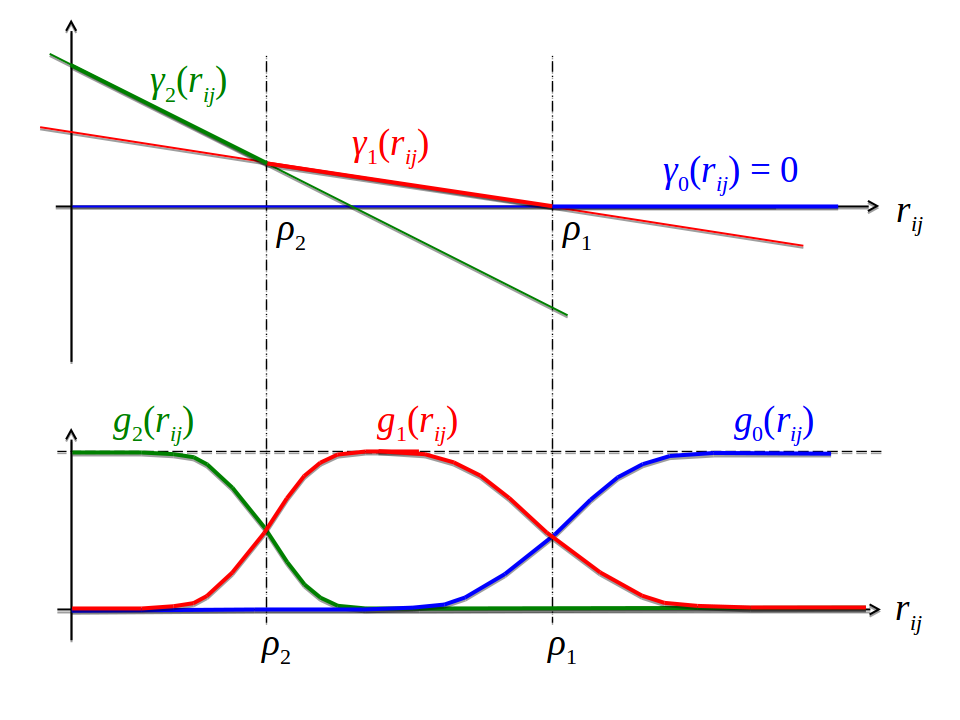
\includegraphics[width=0.5\linewidth]{img/theory/softmax_linear_fct} \caption{The Gaussian mixture coefficients
\(g_k(\rij)\) of \(p(\wij|\rij)\) are modelled as softmax over linear
functions \(\gamma_k(\rij)\). \(\rho_k\) sets the transition point
between neighbouring components \(g_{k-1}(\rij)\) and \(g_k(\rij)\),
while \(\alpha_k\) quantifies the abruptness of the transition between
\(g_{k-1}(\rij)\) and \(g_k(\rij)\).}\label{fig:softmax-linear-fct}
\end{figure}

The functions \(g_k(\rij)\) remain invariant when adding an offset to
all \(\gamma_k(\rij)\). This degeneracy can be removed by setting
\(\gamma_0(\rij) = 0\) (i.e., \(\alpha_0 = 0\) and \(\rho_0=0\)).
Further, the components are ordered, \(\rho_1> \ldots > \rho_K\) and it
is demanded that \(\alpha_k > 0\) for all \(k\). This ensures that for
\(\rij \rightarrow \infty\) we will obtain \(g_0(\rij) \rightarrow 1\)
and hence \(p(\w | \X) \rightarrow \Gauss(0, \sigma_0^2 \I )\).

The parameters \(\rho_k\) mark the transition points between the two
Gaussian mixture components \(k-1\) and \(k\), i.e., the points at which
the two components obtain equal weights. This follows from
\(\gamma_k(\rij) - \gamma_{k-1}(r) = \alpha_{t} ( \rij - \rho_{t})\) and
hence \(\gamma_{k-1}(\rho_k) = \gamma_k(\rho_k)\). A change in
\(\rho_k\) or \(\alpha_k\) only changes the behaviour of
\(g_{k-1}(\rij)\) and \(g_k(\rij)\) in the transition region around
\(\rho_k\). Therefore, this particular definition of \(\gamma_k(\rij)\)
makes the parameters \(\alpha_k\) and \(\rho_k\) as independent of each
other as possible, rendering the optimisation of these parameters more
efficient.

\subsection{\texorpdfstring{Training the Hyperparameters \(\rho_k\) and
\(\alpha_k\) for distance-dependent
prior}{Training the Hyperparameters \textbackslash{}rho\_k and \textbackslash{}alpha\_k for distance-dependent prior}}\label{training-the-hyperparameters-rho_k-and-alpha_k-for-distance-dependent-prior}

\section{Training Random Forest Contat
Prior}\label{training-random-forest-contat-prior}

\subsection{Sequence Derived Features}\label{seq-features}

Given a multiple sequence alignment of a protein family, various
sequence features can be derived that have been found to be informative
of a residue-residue contact.

In total there are \textbf{250} features that can be divided into
global, single position and pairwise features and are described in the
following sections. If not stated otherwise, \emph{weighted} features
have been computed using amino acid counts or amino acid frequencies
based on weighted sequences as described in section
\ref{seq-reweighting}.

\subsubsection{Global Features}\label{seq-features-global}

These features describe alignment characteristics. Every pair of
residues \((i,j)\) from the same protein will be attributed the same
feature.

\begin{longtable}[]{@{}rlc@{}}
\caption{Features characterizing the total alignment}\tabularnewline
\toprule
\begin{minipage}[b]{0.23\columnwidth}\raggedleft\strut
Feature\strut
\end{minipage} & \begin{minipage}[b]{0.50\columnwidth}\raggedright\strut
Description\strut
\end{minipage} & \begin{minipage}[b]{0.18\columnwidth}\centering\strut
No. Features per residue pair \((i, j)\)\strut
\end{minipage}\tabularnewline
\midrule
\endfirsthead
\toprule
\begin{minipage}[b]{0.23\columnwidth}\raggedleft\strut
Feature\strut
\end{minipage} & \begin{minipage}[b]{0.50\columnwidth}\raggedright\strut
Description\strut
\end{minipage} & \begin{minipage}[b]{0.18\columnwidth}\centering\strut
No. Features per residue pair \((i, j)\)\strut
\end{minipage}\tabularnewline
\midrule
\endhead
\begin{minipage}[t]{0.23\columnwidth}\raggedleft\strut
L\strut
\end{minipage} & \begin{minipage}[t]{0.50\columnwidth}\raggedright\strut
log of protein length\strut
\end{minipage} & \begin{minipage}[t]{0.18\columnwidth}\centering\strut
1\strut
\end{minipage}\tabularnewline
\begin{minipage}[t]{0.23\columnwidth}\raggedleft\strut
N\strut
\end{minipage} & \begin{minipage}[t]{0.50\columnwidth}\raggedright\strut
number of sequences\strut
\end{minipage} & \begin{minipage}[t]{0.18\columnwidth}\centering\strut
1\strut
\end{minipage}\tabularnewline
\begin{minipage}[t]{0.23\columnwidth}\raggedleft\strut
Neff\strut
\end{minipage} & \begin{minipage}[t]{0.50\columnwidth}\raggedright\strut
number of effective sequences Neff computed as the sum over sequence
weights (see section \ref{seq-reweighting})\strut
\end{minipage} & \begin{minipage}[t]{0.18\columnwidth}\centering\strut
1\strut
\end{minipage}\tabularnewline
\begin{minipage}[t]{0.23\columnwidth}\raggedleft\strut
gaps\strut
\end{minipage} & \begin{minipage}[t]{0.50\columnwidth}\raggedright\strut
average percentage of gaps over all positions\strut
\end{minipage} & \begin{minipage}[t]{0.18\columnwidth}\centering\strut
1\strut
\end{minipage}\tabularnewline
\begin{minipage}[t]{0.23\columnwidth}\raggedleft\strut
diversity\strut
\end{minipage} & \begin{minipage}[t]{0.50\columnwidth}\raggedright\strut
\(\frac{\sqrt{N}}{L}\), N=number of sequences, L=protein length\strut
\end{minipage} & \begin{minipage}[t]{0.18\columnwidth}\centering\strut
1\strut
\end{minipage}\tabularnewline
\begin{minipage}[t]{0.23\columnwidth}\raggedleft\strut
amino acid composition\strut
\end{minipage} & \begin{minipage}[t]{0.50\columnwidth}\raggedright\strut
weighted amino acid frequencies in alignment\strut
\end{minipage} & \begin{minipage}[t]{0.18\columnwidth}\centering\strut
20\strut
\end{minipage}\tabularnewline
\begin{minipage}[t]{0.23\columnwidth}\raggedleft\strut
secondary structure prediction\strut
\end{minipage} & \begin{minipage}[t]{0.50\columnwidth}\raggedright\strut
average three state propensities PSIPRED
(v4.0){[}\protect\hyperlink{ref-Jones1999}{18}{]}\strut
\end{minipage} & \begin{minipage}[t]{0.18\columnwidth}\centering\strut
3\strut
\end{minipage}\tabularnewline
\begin{minipage}[t]{0.23\columnwidth}\raggedleft\strut
secondary structure prediction\strut
\end{minipage} & \begin{minipage}[t]{0.50\columnwidth}\raggedright\strut
average three state propensities Netsurfp
(v1.0){[}\protect\hyperlink{ref-Petersen2009a}{17}{]}\strut
\end{minipage} & \begin{minipage}[t]{0.18\columnwidth}\centering\strut
3\strut
\end{minipage}\tabularnewline
\begin{minipage}[t]{0.23\columnwidth}\raggedleft\strut
contact prior protein length\strut
\end{minipage} & \begin{minipage}[t]{0.50\columnwidth}\raggedright\strut
simple contact predictor based on expected number of contacts per
protein with respect to protein length (see next subsection
\ref{contact-prior-protein-length})\strut
\end{minipage} & \begin{minipage}[t]{0.18\columnwidth}\centering\strut
1\strut
\end{minipage}\tabularnewline
\bottomrule
\end{longtable}

There are in total \textbf{32} global alignment features.

\subsubsection{Single Position Features}\label{seq-features-single}

These features describe characteristics of a single alignment column.
Every residue pair \((i,j)\) will be described by two features, once for
each position.

\begin{longtable}[]{@{}rlc@{}}
\caption{Single Position Sequence Features}\tabularnewline
\toprule
\begin{minipage}[b]{0.23\columnwidth}\raggedleft\strut
Feature\strut
\end{minipage} & \begin{minipage}[b]{0.50\columnwidth}\raggedright\strut
Description\strut
\end{minipage} & \begin{minipage}[b]{0.18\columnwidth}\centering\strut
No. Features per residue pair \((i, j)\)\strut
\end{minipage}\tabularnewline
\midrule
\endfirsthead
\toprule
\begin{minipage}[b]{0.23\columnwidth}\raggedleft\strut
Feature\strut
\end{minipage} & \begin{minipage}[b]{0.50\columnwidth}\raggedright\strut
Description\strut
\end{minipage} & \begin{minipage}[b]{0.18\columnwidth}\centering\strut
No. Features per residue pair \((i, j)\)\strut
\end{minipage}\tabularnewline
\midrule
\endhead
\begin{minipage}[t]{0.23\columnwidth}\raggedleft\strut
shannon entropy (20 states)\strut
\end{minipage} & \begin{minipage}[t]{0.50\columnwidth}\raggedright\strut
\(- \sum_{a=1}^{20} p_a \log p_a\)\strut
\end{minipage} & \begin{minipage}[t]{0.18\columnwidth}\centering\strut
2\strut
\end{minipage}\tabularnewline
\begin{minipage}[t]{0.23\columnwidth}\raggedleft\strut
shannon entropy (21 states)\strut
\end{minipage} & \begin{minipage}[t]{0.50\columnwidth}\raggedright\strut
\(- \sum_{a=1}^{21} p_a \log p_a\)\strut
\end{minipage} & \begin{minipage}[t]{0.18\columnwidth}\centering\strut
2\strut
\end{minipage}\tabularnewline
\begin{minipage}[t]{0.23\columnwidth}\raggedleft\strut
kullback leibler divergence\strut
\end{minipage} & \begin{minipage}[t]{0.50\columnwidth}\raggedright\strut
between weighted observed and background amino acid frequencies
{[}\protect\hyperlink{ref-Robinson1991}{35}{]}\strut
\end{minipage} & \begin{minipage}[t]{0.18\columnwidth}\centering\strut
2\strut
\end{minipage}\tabularnewline
\begin{minipage}[t]{0.23\columnwidth}\raggedleft\strut
jennson shannon divergence\strut
\end{minipage} & \begin{minipage}[t]{0.50\columnwidth}\raggedright\strut
between weighted observed and background amino acid frequencies
{[}\protect\hyperlink{ref-Robinson1991}{35}{]}\strut
\end{minipage} & \begin{minipage}[t]{0.18\columnwidth}\centering\strut
2\strut
\end{minipage}\tabularnewline
\begin{minipage}[t]{0.23\columnwidth}\raggedleft\strut
PSSM\strut
\end{minipage} & \begin{minipage}[t]{0.50\columnwidth}\raggedright\strut
log odds ratio of weighted observed and background amino acid
frequencies {[}\protect\hyperlink{ref-Robinson1991}{35}{]}\strut
\end{minipage} & \begin{minipage}[t]{0.18\columnwidth}\centering\strut
40\strut
\end{minipage}\tabularnewline
\begin{minipage}[t]{0.23\columnwidth}\raggedleft\strut
secondary structure prediction\strut
\end{minipage} & \begin{minipage}[t]{0.50\columnwidth}\raggedright\strut
three state propensities PSIPRED (v4.0)
{[}\protect\hyperlink{ref-Jones1999}{18}{]}\strut
\end{minipage} & \begin{minipage}[t]{0.18\columnwidth}\centering\strut
6\strut
\end{minipage}\tabularnewline
\begin{minipage}[t]{0.23\columnwidth}\raggedleft\strut
secondary structure prediction\strut
\end{minipage} & \begin{minipage}[t]{0.50\columnwidth}\raggedright\strut
three state propensities Netsurfp (v1.0)
{[}\protect\hyperlink{ref-Petersen2009a}{17}{]}\strut
\end{minipage} & \begin{minipage}[t]{0.18\columnwidth}\centering\strut
6\strut
\end{minipage}\tabularnewline
\begin{minipage}[t]{0.23\columnwidth}\raggedleft\strut
solvent accessibility prediction\strut
\end{minipage} & \begin{minipage}[t]{0.50\columnwidth}\raggedright\strut
RSA and RSA Z-score Netsurfp (v1.0)
{[}\protect\hyperlink{ref-Petersen2009a}{17}{]}\strut
\end{minipage} & \begin{minipage}[t]{0.18\columnwidth}\centering\strut
4\strut
\end{minipage}\tabularnewline
\begin{minipage}[t]{0.23\columnwidth}\raggedleft\strut
relative position in sequence\strut
\end{minipage} & \begin{minipage}[t]{0.50\columnwidth}\raggedright\strut
\(\frac{i}{L}\) for a protien of length \(L\)\strut
\end{minipage} & \begin{minipage}[t]{0.18\columnwidth}\centering\strut
2\strut
\end{minipage}\tabularnewline
\begin{minipage}[t]{0.23\columnwidth}\raggedleft\strut
number of ungapped sequences\strut
\end{minipage} & \begin{minipage}[t]{0.50\columnwidth}\raggedright\strut
\(\sum_n w_n I(x_{ni} \neq 20)\) for sequences \(x_n\) and sequence
weights \(w_n\)\strut
\end{minipage} & \begin{minipage}[t]{0.18\columnwidth}\centering\strut
2\strut
\end{minipage}\tabularnewline
\begin{minipage}[t]{0.23\columnwidth}\raggedleft\strut
percentage of gaps\strut
\end{minipage} & \begin{minipage}[t]{0.50\columnwidth}\raggedright\strut
\(\frac{\sum_n w_n I(x_{ni} = 20)}{N_{\text{eff}}}\) for sequences
\(x_n\) and sequence weights \(w_n\)\strut
\end{minipage} & \begin{minipage}[t]{0.18\columnwidth}\centering\strut
2\strut
\end{minipage}\tabularnewline
\begin{minipage}[t]{0.23\columnwidth}\raggedleft\strut
Average physico-chemical properties\strut
\end{minipage} & \begin{minipage}[t]{0.50\columnwidth}\raggedright\strut
Atchley Factors 1-5 {[}\protect\hyperlink{ref-Atchley2005}{36}{]}\strut
\end{minipage} & \begin{minipage}[t]{0.18\columnwidth}\centering\strut
10\strut
\end{minipage}\tabularnewline
\begin{minipage}[t]{0.23\columnwidth}\raggedleft\strut
Average physico-chemical properties\strut
\end{minipage} & \begin{minipage}[t]{0.50\columnwidth}\raggedright\strut
Polarity according to Grantham, 1974. Data taken from
\href{http://www.genome.jp/dbget-bin/www_bget?aaindex:GRAR740102}{AAindex
Database} {[}\protect\hyperlink{ref-Kawashima2008}{37}{]}.\strut
\end{minipage} & \begin{minipage}[t]{0.18\columnwidth}\centering\strut
2\strut
\end{minipage}\tabularnewline
\begin{minipage}[t]{0.23\columnwidth}\raggedleft\strut
Average physico-chemical properties\strut
\end{minipage} & \begin{minipage}[t]{0.50\columnwidth}\raggedright\strut
Polarity according to Zimmermann et al., 1986. Data taken from
\href{http://www.genome.jp/dbget-bin/www_bget?aaindex:ZIMJ680103}{AAindex
Database} {[}\protect\hyperlink{ref-Kawashima2008}{37}{]}.\strut
\end{minipage} & \begin{minipage}[t]{0.18\columnwidth}\centering\strut
2\strut
\end{minipage}\tabularnewline
\begin{minipage}[t]{0.23\columnwidth}\raggedleft\strut
Average physico-chemical properties\strut
\end{minipage} & \begin{minipage}[t]{0.50\columnwidth}\raggedright\strut
Isoelectric point according to Zimmermann et al., 1968. Data taken from
\href{http://www.genome.jp/dbget-bin/www_bget?aaindex:ZIMJ680104}{AAindex
Database} {[}\protect\hyperlink{ref-Kawashima2008}{37}{]}.\strut
\end{minipage} & \begin{minipage}[t]{0.18\columnwidth}\centering\strut
2\strut
\end{minipage}\tabularnewline
\begin{minipage}[t]{0.23\columnwidth}\raggedleft\strut
Average physico-chemical properties\strut
\end{minipage} & \begin{minipage}[t]{0.50\columnwidth}\raggedright\strut
Hydrophobicity scale according to Wimley \& White, 1996. Data taken from
\href{https://www.cgl.ucsf.edu/chimera/docs/ContributedSoftware/defineattrib/wwHydrophobicity.txt}{UCSF
Chimera} {[}\protect\hyperlink{ref-Wimley1996}{38}{]}.\strut
\end{minipage} & \begin{minipage}[t]{0.18\columnwidth}\centering\strut
2\strut
\end{minipage}\tabularnewline
\begin{minipage}[t]{0.23\columnwidth}\raggedleft\strut
Average physico-chemical properties\strut
\end{minipage} & \begin{minipage}[t]{0.50\columnwidth}\raggedright\strut
Hydrophobicity index according to Kyte \& Doolittle, 1982. Data taken
from
\href{http://www.genome.jp/dbget-bin/www_bget?aaindex:KYTJ820101}{AAindex
Database} {[}\protect\hyperlink{ref-Kawashima2008}{37}{]}.\strut
\end{minipage} & \begin{minipage}[t]{0.18\columnwidth}\centering\strut
2\strut
\end{minipage}\tabularnewline
\begin{minipage}[t]{0.23\columnwidth}\raggedleft\strut
Average physico-chemical properties\strut
\end{minipage} & \begin{minipage}[t]{0.50\columnwidth}\raggedright\strut
Hydrophobicity according to Cornette
{[}\protect\hyperlink{ref-Cornette1987}{39}{]}.\strut
\end{minipage} & \begin{minipage}[t]{0.18\columnwidth}\centering\strut
2\strut
\end{minipage}\tabularnewline
\begin{minipage}[t]{0.23\columnwidth}\raggedleft\strut
Average physico-chemical properties\strut
\end{minipage} & \begin{minipage}[t]{0.50\columnwidth}\raggedright\strut
Bulkiness according to Zimmerman et al., 1968. Data taken from
\href{http://www.genome.jp/dbget-bin/www_bget?aaindex:ZIMJ680102}{AAindex
Database} {[}\protect\hyperlink{ref-Kawashima2008}{37}{]}.\strut
\end{minipage} & \begin{minipage}[t]{0.18\columnwidth}\centering\strut
2\strut
\end{minipage}\tabularnewline
\begin{minipage}[t]{0.23\columnwidth}\raggedleft\strut
Average physico-chemical properties\strut
\end{minipage} & \begin{minipage}[t]{0.50\columnwidth}\raggedright\strut
Average volumes of residues according to Pontius et al., 1996. Data
taken from
\href{http://www.genome.jp/dbget-bin/www_bget?aaindex:PONJ960101}{AAindex
Database} {[}\protect\hyperlink{ref-Kawashima2008}{37}{]}.\strut
\end{minipage} & \begin{minipage}[t]{0.18\columnwidth}\centering\strut
2\strut
\end{minipage}\tabularnewline
\bottomrule
\end{longtable}

There are in total \textbf{96} single sequence features.

Additionally, all single features will be computed within a window of
size 5. The window feature for center residue \(i\) will be computed as
the mean feature over residues \([i-2, \ldots, i, \ldots, i+2]\).
Whenever the window extends the range of the sequence (for \(i\!<\!2\)
and \(i\!>\!(L-2)\)), the window feature will be computed only for valid
sequence positions. This results in additional \textbf{96} window
features.

\subsubsection{Pairwise Features}\label{seq-features-pairwise}

These features are computed for every pair of columns \((i, j)\) in the
alignment with \(i<j\).

\begin{longtable}[]{@{}rlc@{}}
\caption{Pairwise Sequence Features}\tabularnewline
\toprule
\begin{minipage}[b]{0.23\columnwidth}\raggedleft\strut
Feature\strut
\end{minipage} & \begin{minipage}[b]{0.50\columnwidth}\raggedright\strut
Description\strut
\end{minipage} & \begin{minipage}[b]{0.18\columnwidth}\centering\strut
No. Features per residue pair \((i, j)\)\strut
\end{minipage}\tabularnewline
\midrule
\endfirsthead
\toprule
\begin{minipage}[b]{0.23\columnwidth}\raggedleft\strut
Feature\strut
\end{minipage} & \begin{minipage}[b]{0.50\columnwidth}\raggedright\strut
Description\strut
\end{minipage} & \begin{minipage}[b]{0.18\columnwidth}\centering\strut
No. Features per residue pair \((i, j)\)\strut
\end{minipage}\tabularnewline
\midrule
\endhead
\begin{minipage}[t]{0.23\columnwidth}\raggedleft\strut
sequence separation\strut
\end{minipage} & \begin{minipage}[t]{0.50\columnwidth}\raggedright\strut
\(j-i\)\strut
\end{minipage} & \begin{minipage}[t]{0.18\columnwidth}\centering\strut
1\strut
\end{minipage}\tabularnewline
\begin{minipage}[t]{0.23\columnwidth}\raggedleft\strut
gaps\strut
\end{minipage} & \begin{minipage}[t]{0.50\columnwidth}\raggedright\strut
pairwise percentage of gaps using weighted sequences\strut
\end{minipage} & \begin{minipage}[t]{0.18\columnwidth}\centering\strut
1\strut
\end{minipage}\tabularnewline
\begin{minipage}[t]{0.23\columnwidth}\raggedleft\strut
number of ungapped sequences\strut
\end{minipage} & \begin{minipage}[t]{0.50\columnwidth}\raggedright\strut
\(\sum_n w_n I(x_{ni} \! \neq \! 20, x_{nj} \! \neq \! 20)\) for
sequences \(x_n\) and sequence weights \(w_n\)\strut
\end{minipage} & \begin{minipage}[t]{0.18\columnwidth}\centering\strut
1\strut
\end{minipage}\tabularnewline
\begin{minipage}[t]{0.23\columnwidth}\raggedleft\strut
correlation physico-chemical features\strut
\end{minipage} & \begin{minipage}[t]{0.50\columnwidth}\raggedright\strut
pairwise correlation of all physico-chemical properties listed in
\ref{seq-features-single}\strut
\end{minipage} & \begin{minipage}[t]{0.18\columnwidth}\centering\strut
13\strut
\end{minipage}\tabularnewline
\begin{minipage}[t]{0.23\columnwidth}\raggedleft\strut
pairwise potential\strut
\end{minipage} & \begin{minipage}[t]{0.50\columnwidth}\raggedright\strut
Average quasi-chemical energy of interactions in an average buried
environment. Data taken from
\href{http://www.genome.jp/dbget-bin/www_bget?aaindex:MIYS990107}{AAindex
Database} {[}\protect\hyperlink{ref-Kawashima2008}{37}{]}.\strut
\end{minipage} & \begin{minipage}[t]{0.18\columnwidth}\centering\strut
1\strut
\end{minipage}\tabularnewline
\begin{minipage}[t]{0.23\columnwidth}\raggedleft\strut
pairwise potential\strut
\end{minipage} & \begin{minipage}[t]{0.50\columnwidth}\raggedright\strut
Average quasi-chemical energy of transfer of amino acids from water to
the protein environment. Data taken from
\href{http://www.genome.jp/dbget-bin/www_bget?aaindex:MIYS990106}{AAindex
Database} {[}\protect\hyperlink{ref-Kawashima2008}{37}{]}.\strut
\end{minipage} & \begin{minipage}[t]{0.18\columnwidth}\centering\strut
1\strut
\end{minipage}\tabularnewline
\begin{minipage}[t]{0.23\columnwidth}\raggedleft\strut
pairwise potential\strut
\end{minipage} & \begin{minipage}[t]{0.50\columnwidth}\raggedright\strut
Average general contact potential by Li\&Fang
{[}\protect\hyperlink{ref-Li2011}{16}{]}\strut
\end{minipage} & \begin{minipage}[t]{0.18\columnwidth}\centering\strut
1\strut
\end{minipage}\tabularnewline
\begin{minipage}[t]{0.23\columnwidth}\raggedleft\strut
pairwise potential\strut
\end{minipage} & \begin{minipage}[t]{0.50\columnwidth}\raggedright\strut
Average statistical potential from residue pairs in beta-sheets by
Zhu\&Braun {[}\protect\hyperlink{ref-Zhu1999}{40}{]}\strut
\end{minipage} & \begin{minipage}[t]{0.18\columnwidth}\centering\strut
1\strut
\end{minipage}\tabularnewline
\begin{minipage}[t]{0.23\columnwidth}\raggedleft\strut
joint\_shannon\_entropy (20 state)\strut
\end{minipage} & \begin{minipage}[t]{0.50\columnwidth}\raggedright\strut
\(- \sum_{a=1}^{20}\sum_{b=1}^{20} p(a,b) \log p(a,b)\)\strut
\end{minipage} & \begin{minipage}[t]{0.18\columnwidth}\centering\strut
1\strut
\end{minipage}\tabularnewline
\begin{minipage}[t]{0.23\columnwidth}\raggedleft\strut
joint\_shannon\_entropy (21 state)\strut
\end{minipage} & \begin{minipage}[t]{0.50\columnwidth}\raggedright\strut
\(- \sum_{a=1}^{21}\sum_{b=1}^{21} p(a,b) \log p(a,b)\)\strut
\end{minipage} & \begin{minipage}[t]{0.18\columnwidth}\centering\strut
1\strut
\end{minipage}\tabularnewline
\begin{minipage}[t]{0.23\columnwidth}\raggedleft\strut
mutual information (MI)\strut
\end{minipage} & \begin{minipage}[t]{0.50\columnwidth}\raggedright\strut
mutual information of amino acid counts at two positions; several
variants: MI with pseudo-counts, MI with pseudo-counts +
\protect\hyperlink{abbrev}{APC}, normalized MI\strut
\end{minipage} & \begin{minipage}[t]{0.18\columnwidth}\centering\strut
3\strut
\end{minipage}\tabularnewline
\begin{minipage}[t]{0.23\columnwidth}\raggedleft\strut
OMES\strut
\end{minipage} & \begin{minipage}[t]{0.50\columnwidth}\raggedright\strut
according to Fodor\&Aldrich {[}\protect\hyperlink{ref-Fodor2004a}{14}{]}
with and without \protect\hyperlink{abbrev}{APC}\strut
\end{minipage} & \begin{minipage}[t]{0.18\columnwidth}\centering\strut
2\strut
\end{minipage}\tabularnewline
\bottomrule
\end{longtable}

There are in total \textbf{26} pairwise sequence features.

\subsubsection{Protein length dependent Contact
Prior}\label{contact-prior-protein-length}

The average number of contats per residue, computed as the observed
number of contacts divided by protein length L, has a non-linear
relationship with protein length L as can be seen in Figure
\ref{fig:avg-nr-contacts-per-residue-vs-protein-length}.






\begin{figure}

{\centering 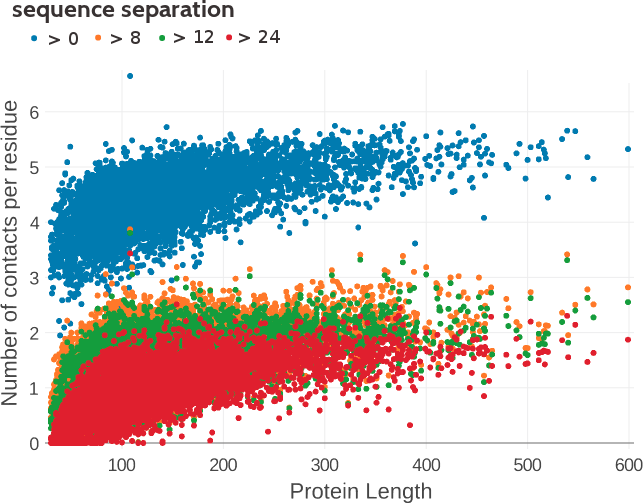
\includegraphics[width=0.8\linewidth]{img/random_forest_contact_prior/no_contacts_per_residue_vs_protein_length_thr8} 

}

\caption{Observed
number of contacts per residue has a non-linear relationship with
protein length. Distribution is shown for several thresholds of sequence
separation.}\label{fig:avg-nr-contacts-per-residue-vs-protein-length}
\end{figure}

In log space, the average number of contats per residue can be fitted
with a linear regression (see Figure
\ref{fig:avg-nr-contacts-per-residue-vs-log-protein-length-linfit}) and
yields the following functions:

\begin{itemize}
\tightlist
\item
  \(f(L) = 1.556 + 0.596 \log (L)\) for sequence separation of 0
  positions
\item
  \(f(L) = -1.273 + 0.59 \log (L)\) for sequence separation of 8
  positions
\item
  \(f(L) = -1.567 + 0.615 \log (L)\) for sequence separation of 12
  positions
\item
  \(f(L) = -2.0 + 0.624 \log (L)\) for sequence separation of 24
  positions
\end{itemize}

A simple contact predictor can be formulated as the ratio of the
expected number of contacts per residue, given by \(f(L)\), and the
possible number of contacts per residue which is \(L-1\),

\[
p(r_{ij} = 1 | L) = \frac{f(L)}{L-1} \; ,
\]

with \(r_{ij}=1\) representing a contact between residue \(i\) and
\(j\).

(ref:caption-avg-nr-contacts-per-residue-vs-log-protein-length-linfit)
Linear regression fits for average number of contats per residue on
logarithm of protein length. Distribution and linear regression fits are
shown for different sequence separation thresholds.

\begin{figure}

{\centering 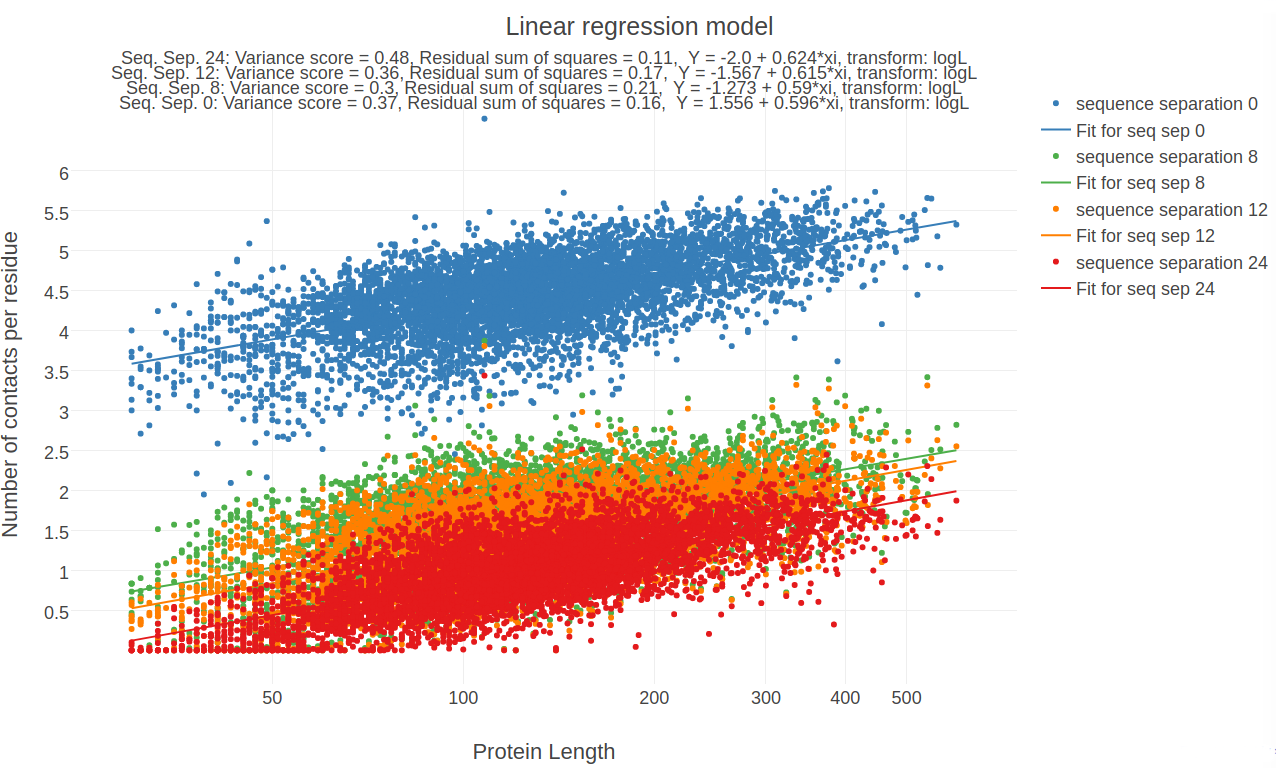
\includegraphics[width=0.9\linewidth]{img/random_forest_contact_prior/model_linreg_transformlogL_no_contacts_per_residue_vs_protein_length_thr8} 

}

\caption{(ref:caption-avg-nr-contacts-per-residue-vs-log-protein-length-linfit)}\label{fig:avg-nr-contacts-per-residue-vs-log-protein-length-linfit}
\end{figure}

\subsection{Hyperparameter Optimization for Random Forest
Prior}\label{rf-hyperparameter-optimization}

There are several hyperparameters in a random forest model that need to
be tuned to achieve best balance between predictive power and runtime.
While more trees in the random forest generally improve performance of
the model, they will slow down training and prediction. A crucial
hyperparamter is the number of features that is randomly selected for a
split at each node in a tree
{[}\protect\hyperlink{ref-Bernard2009}{41}{]}. Stochasticity introduced
by the random selection of features is a key characteristic of random
forests as it reduces correlation between the trees and thus the
variance of the predictor. Selecting many features typically increases
performance as more options can be considered for each split, but at the
same time increases risk of overfitting and decreases speed of the
algorithm. In general, random forests are robust to overfitting, as long
as there are enough trees in the ensemble and the selection of features
for splitting a node introduces sufficient stochasticity. Overfitting
can furthermore be prevented by restricting the depth of the trees,
which is known as pruning or by enforcing a minimal node size with
respect to the number of features per node. A positive side-effect of
taking these measures is a speedup of the algorithm.
{[}\protect\hyperlink{ref-Louppe2014}{12}{]}

In the following, I use 5-fold cross-validation to identify the optimal
architecture of the random forest. I used the module
\href{http://scikit-learn.org/stable/modules/generated/sklearn.ensemble.RandomForestClassifier.html\#sklearn.ensemble.RandomForestClassifier}{RandomForestClassifier}
in the Python package \texttt{sklearn\ (v.\ 0.19)}
{[}\protect\hyperlink{ref-Pedregosa2011}{42}{]} and trained the models
on sequence features extracted from \protect\hyperlink{abbrev}{MSAs} as
described in section \ref{seq-features}. Single position features are
computed with a window of size five as described in section
\ref{seq-features-single}.

Proteins constitute highly imbalanced datasets with respect to the
number of residue pairs that form and form not physical contacts. As can
be seen in Figure \ref{fig:fraction-contacts-vs-protein-length},
depending on the enforced sequence separation threshold the percentage
of contacts varies between approximately 1\% and 5\%.








\begin{figure}

{\centering 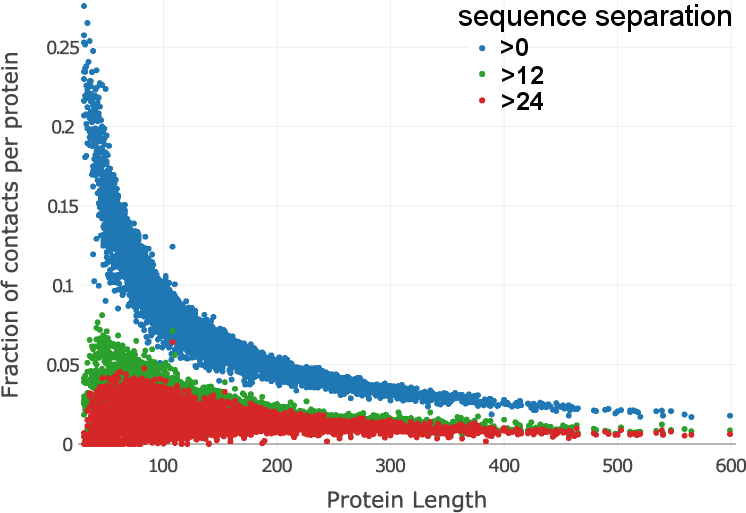
\includegraphics[width=0.8\linewidth]{img/random_forest_contact_prior/fraction_contacts_vs_protein_length_thr8} 

}

\caption{Fraction of contacts
among all possible contacts (\(\frac{L(L-1)}{2}\)) in a protein against
protein length L. The distribution has a non-linear relationship. At a
sequence separation threshold \textgreater{}8 positions the fraction of
contacts for intermediate size proteins with length \textgreater{}100 is
approximately 2\%.}\label{fig:fraction-contacts-vs-protein-length}
\end{figure}














\begin{figure}

{\centering 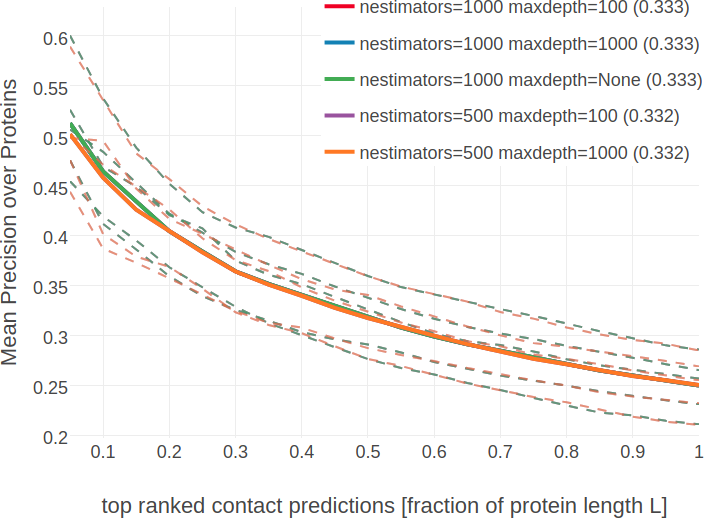
\includegraphics[width=1\linewidth]{img/random_forest_contact_prior/new_gridsearch/precision_vs_rank_cv_on_test_random_forest_nestimators_maxdepth_top5_notitle} 

}

\caption{Mean precision over
200 proteins against highest scoring contact predictions from random
forest models for different settings of \emph{n\_estimators} and
\emph{max\_depth}. Dashed lines show the performance of models that have
been learned on the five different subsets of training data. Solid lines
give the mean precision over the five models. Only those models are
shown that yielded the five highest mean precision values (given in
parantheses in the legend). Random forest models with 1000 trees and
maximum depth of trees of either 100, 1000 or unrestricted tree depth
perform nearly identical (lines overlap). Random forest models with 500
trees and \emph{max\_depth}=10 or \emph{max\_depth}=100 perform slightly
worse.}\label{fig:rf-gridsearch-nestimators-maxfeatures}
\end{figure}

Most studies applying machine learning algorithms to the problem of
predicting residue-residue contacts, chose the standard approach of
rebalancing the data set by undersampling of the majority class.

\begin{longtable}[]{@{}rcc@{}}
\toprule
Study & Proportion of Contacts & Proportion of
Non-contacts\tabularnewline
\midrule
\endhead
Wu et al. (2008) {[}\protect\hyperlink{ref-Wu2008}{43}{]} & 1 &
4\tabularnewline
Li et al. (2011) {[}\protect\hyperlink{ref-Li2011}{16}{]} & 1 & 1,
2\tabularnewline
Wang et al. (2011) {[}\protect\hyperlink{ref-Wang2011}{44}{]} & 1 &
4\tabularnewline
DiLena et al. (2012) {[}\protect\hyperlink{ref-DiLena2012a}{45}{]} & 1 &
\textasciitilde{}4\tabularnewline
Wang et al. (2013) {[}\protect\hyperlink{ref-Wang2013}{46}{]} & 1 &
\textasciitilde{}4\tabularnewline
\bottomrule
\end{longtable}

I followed the same strategy and undersampled residue pairs that are not
physical contacts with a proportion of contacts to non-contacts of 1:5.
The training set is comprised of 50.000 residue pairs \(< 8 \angstrom\)
(``contacts''``) and 250.000 residue pairs \(> 8 \angstrom\)
(''non-contacts``) so that each of the five cross-validation models will
be trained on 40.000 contacts and 200.000 non-contacts. As the training
set has been undersampled for non-contacts, it is not representative of
real world proteins and the models should be validated on a more
realistic validation set. Each of the five models is therefore
cross-validated on an own independent dataset of residue pairs extracted
from 40 proteins by means of the standard contact prediction benchmark
(mean precision against top ranked contacts).

\pagebreak

First I assessed performance of models for combinations of the parameter
\emph{n\_estimators}, defining the number of trees in the forest and the
parameter \emph{max\_depth} defining the maximum depth of the trees:

\begin{itemize}
\tightlist
\item
  \emph{n\_estimators} \(\in \{100,500,1000\}\)
\item
  \emph{max\_depth} \(\in \{10, 100, 1000, None\}\)
\end{itemize}

Figure \ref{fig:rf-gridsearch-nestimators-maxfeatures} shows that the
top five parameter combinations perform nearly identical. Random forests
with 1000 trees perform slightly better than models constituting 500
trees, irrespective of the depth of the trees. In order to keep model
complexity small, \texttt{n\_estimators=1000} and
\texttt{max\_depth=100} for further analysis.

Next, I optimized the parameters \emph{min\_samples\_leaf}, defining the
minimum number of samples required to be at a leaf node and
\emph{max\_features}, defining the number of randomly selected features
considered for each split using the following settings:

\begin{itemize}
\tightlist
\item
  \emph{min\_samples\_leaf} \(\in \{1, 10, 100\}\)
\item
  \emph{max\_features} \(\in \{\text{sqrt}, \text{log2}, 0.15, 0.3\}\)
\end{itemize}

Randomly selecting 39\% of features (=75 features) and requiring at
least 10 samples per leaf gives highest mean precision as can be seen in
Figure \ref{fig:rf-gridsearch-maxdepth-minsampleleaf}. I chose
\texttt{max\_features\ =\ 0.30} and \texttt{min\_samples\_leaf\ =\ 10}
for further analysis. Tuning the hyperparameters in a different order or
on a larger dataset gives similar results.










\begin{figure}

{\centering 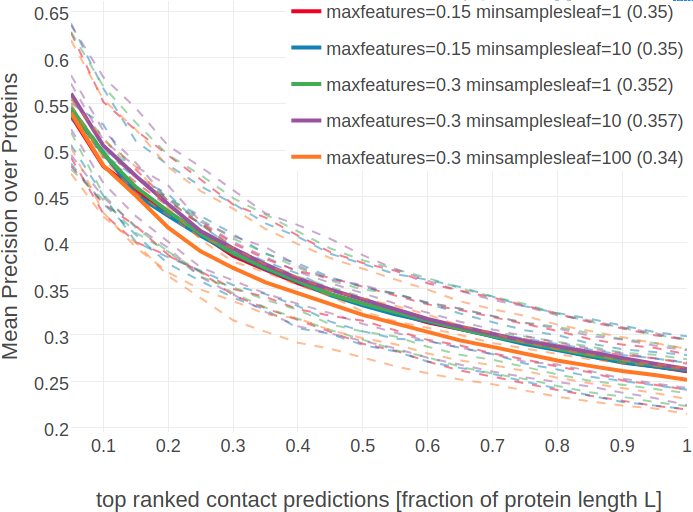
\includegraphics[width=1\linewidth]{img/random_forest_contact_prior/new_gridsearch/precision_vs_rank_cv_on_test_random_forest_maxfeatures_minsampleleaf_top5_notitle} 

}

\caption{Mean precision over 200
proteins against highest scoring contact predictions from random forest
models with different settings of \emph{min\_samples\_leaf} and
\emph{max\_features}. Dashed lines show the performance of models that
have been learned on the five different subsets of training data. Solid
lines give the mean precision over the five models. Only those models
are shown that yielded the five best mean precision values (given in
parantheses in the legend).}\label{fig:rf-gridsearch-maxdepth-minsampleleaf}
\end{figure}

In a next step I assessed dataset specific settings, such as the window
size over which single positions features will be computed, the distance
threshold to define non-contacts and the optimal proportions of contacts
and non-contacts in the training set. I used the previously identified
settings of random forest hyperparameters
(\texttt{n\_estimators=1000,\ min\_samples\_leaf=10,\ max\_depth=100,\ max\_features=0.30}).

\begin{itemize}
\tightlist
\item
  ratio of non-contacts/contacts \(\in \{2, 5, 10, 20 \}\) within a
  fixed total dataset size of 300 000 residue pairs
\item
  window size: \(\in \{5, 7, 9, 11\}\)
\item
  non-contact threshold \(\in \{8, 15, 20\}\)
\end{itemize}

As can be seen in appendix \ref{rf-window-size} and
\ref{rf-noncontact-threshold}, the default choice of using a window size
of five positions and the non-contact threshold of \(8 \angstrom\)
proves to be the optimal setting. Furthermore, using five-times as many
non-contacts as contacts in the training set results in highest mean
precision as can be seen in appendix \ref{rf-ratio-noncontacts}. These
estimates might be biased in a way since the random forest
hyperparameters have been optimized on a dataset using exactly these
optimal settings.

\subsection{Feature Selection}\label{rf-feature-selection}

Many features obtain low \emph{Gini importance} scores and can most
likely be removed from the data set which will also reduce model
complexity. It has been found, that prediction performance might even
increase after removing the most irrelevant features
{[}\protect\hyperlink{ref-Menze2009}{11}{]}. For example, during the
development of \emph{EPSILON-CP}, a deep neural network method for
contact prediction, the authors performed feature selection using
boosted trees. By removing 75\% of the most non-informative features
(mostly features related to amino acid composition), the performance of
their predictor increased slightly
{[}\protect\hyperlink{ref-Stahl2017}{5}{]}. Other studies have also
emphasized the importance of feature selection to improve performance
and reduce model complexity
{[}\protect\hyperlink{ref-Li2011}{16},\protect\hyperlink{ref-Cheng2007}{47}{]}.

I therefore developed a feature selection pipeline that retrains the
random forest model on subsets of features. The subsets are composed of
those features having \emph{Gini importance} larger than the
\(\{10, 30, 50, 70, 90\}\)-percentile of the distribution of \emph{Gini
importance} values obtained by training a model on all features.
Performance of the models trained on these subsets of features is
evaluated on a validation set.

\subsection{Using Pseudo-likelihood Coevolution Score as Additional
Feature}\label{rf-with-pll-score}

Besides the 250 sequence derived features, the pseudo-likelihood contact
score (\protect\hyperlink{abbrev}{APC} corrected Frobenius norm of
couplings) is used as an additional feature. The random forest was
trained on 100.000 residue pairs in physical contact
(\(\Delta \Cb < 8 \angstrom \; \;\)) and 500.000 residue pairs not in
physical contact (\(\Delta \Cb > 8 \angstrom \; \;\)) using the
cross-validated hyperparameters as described earlier.

The pseudo-likelihood contact score comprises by far the most important
feature as can be seen in the Figure
\ref{fig:feature-importance-rf-with-pll-score}. Other important features
include the local statistical contact scores OMES and mutual
information, the mean pairwise potentials according to Miyasawa \&
Jernigan {[}\protect\hyperlink{ref-Miyazawa1999a}{15}{]} and Li \& Fang
{[}\protect\hyperlink{ref-Li2011}{16}{]}, relative solvent accessibilty
predictions (with NetsurfP
{[}\protect\hyperlink{ref-Petersen2009a}{17}{]}). The most important
features apart from the pseudo-likelihood contact score, are the same
features that are highly relevant for the basic random forest model (see
Figure \ref{fig:rf-feature-importance}).

























\begin{figure}

{\centering 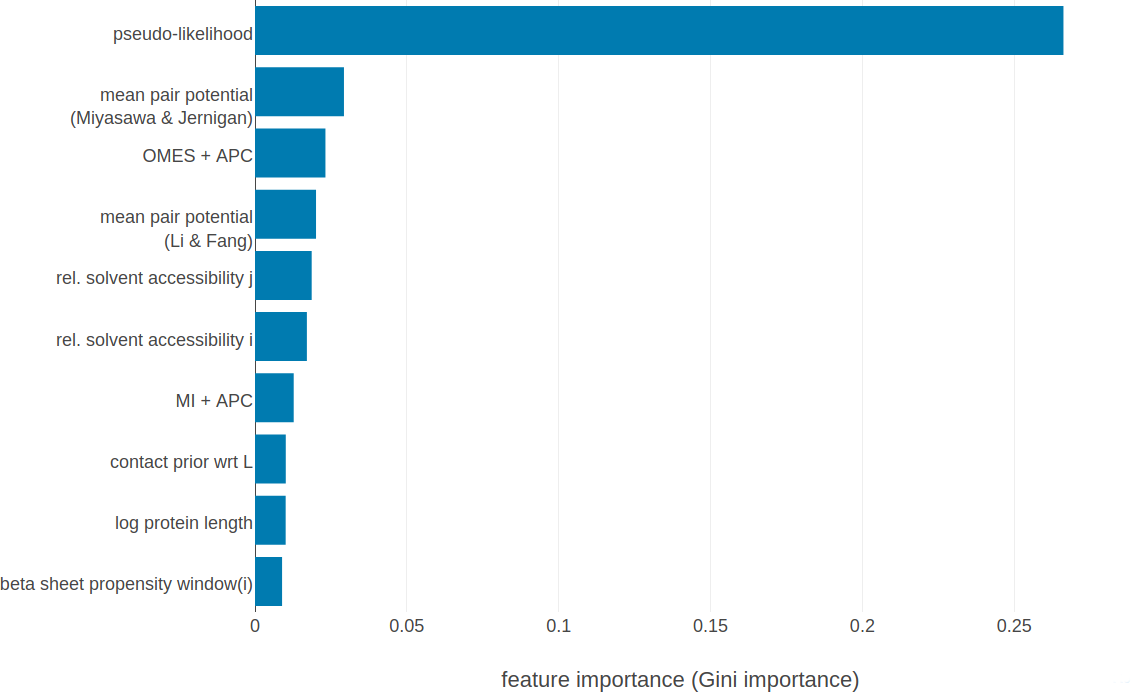
\includegraphics[width=1\linewidth]{img/random_forest_contact_prior/pll_feature/feature_random_forest_top_pLLfeature} 

}

\caption{Top ten features
ranked according to \emph{Gini importance}. \textbf{pseudo-likelihood}:
\protect\hyperlink{abbrev}{APC} corrected Frobenius norm of couplings
computed with pseudo-likelihood. \textbf{mean pair potential (Miyasawa
\& Jernigan)}: average quasi-chemical energy of transfer of amino acids
from water to the protein environment
{[}\protect\hyperlink{ref-Miyazawa1999a}{15}{]}. \textbf{OMES+APC}:
\protect\hyperlink{abbrev}{APC} corrected OMES score according to
Fodor\&Aldrich {[}\protect\hyperlink{ref-Fodor2004a}{14}{]}.
\textbf{mean pair potential (Li\&Fang)}: average general contact
potential by Li \& Fang {[}\protect\hyperlink{ref-Li2011}{16}{]}.
\textbf{rel. solvent accessibilty i(j)}: RSA score computed with
Netsurfp (v1.0) {[}\protect\hyperlink{ref-Petersen2009a}{17}{]} for
position i(j). \textbf{MI+APC}: \protect\hyperlink{abbrev}{APC}
corrected mutual information between amino acid counts (using
pseudo-counts). \textbf{contact prior wrt L}: simple contact prior based
on expected number of contacts wrt protein length (see methods section
\ref{contact-prior-protein-length}). \textbf{log protein length}:
logarithm of protein length. \textbf{beta sheet propensity window(i)}:
beta-sheet propensity according to Psipred
{[}\protect\hyperlink{ref-Jones1999}{18}{]} computed within a window of
five positions around i. Features are described in detail in methods
section \ref{seq-features}.}\label{fig:feature-importance-rf-with-pll-score}
\end{figure}

Models that have been trained on subsets of features, comprising 226,
176, 126 or 76 of the most important features with respect to \emph{Gini
importance}, perform equally well as the model trained on the complete
set of features (see Figure
\ref{fig:feature-selection-rf-with-pll-score}). Only the model trained
on the 26 most important features has slighlty decreased precision for
the top L/10 ranked contacts.






\begin{figure}

{\centering 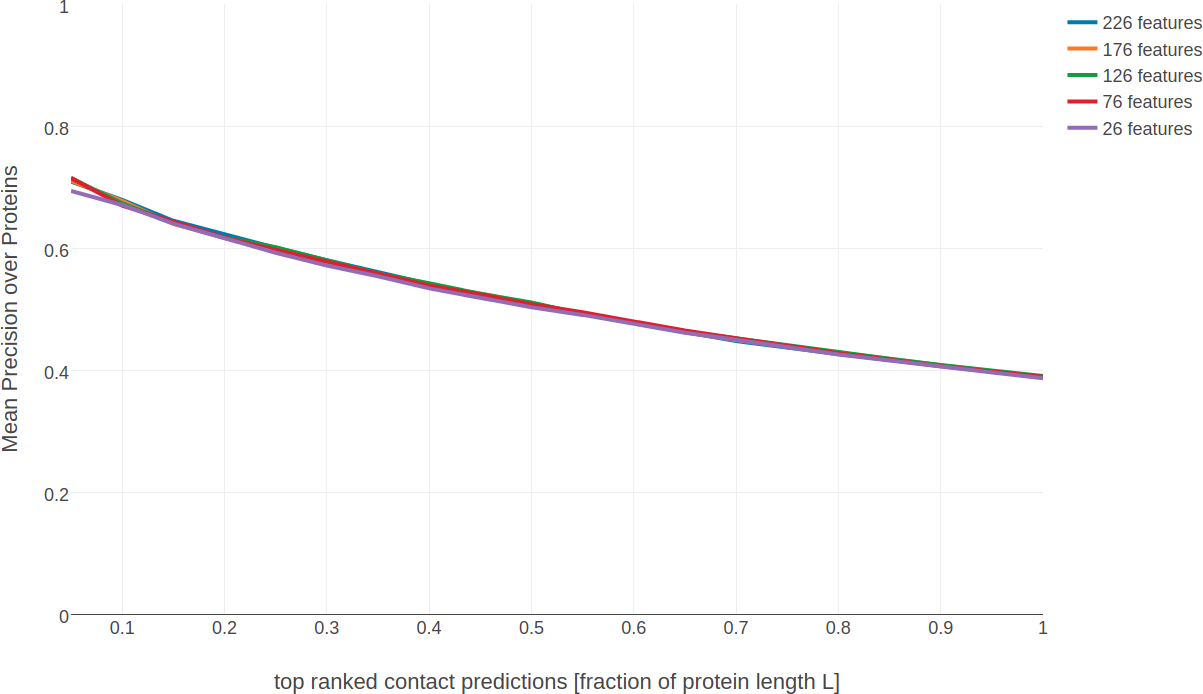
\includegraphics[width=1\linewidth]{img/random_forest_contact_prior/pll_feature/precision_vs_rank_featureselection_random_forest_nestimators1000_maxfeatures03_maxdepth100_minsamplesleaf10_pLLfeature} 

}

\caption{Mean precision for top
ranked contacts over 200 proteins for variaous random forest models
trained on subsets of features. Subsets of features have been selected
as described in section \ref{rf-feature-selection}.}\label{fig:feature-selection-rf-with-pll-score}
\end{figure}

\appendix


\hypertarget{abbrev}{\chapter{Abbreviations}\label{abbrev}}

\textbf{APC} Avarage Product Correction

\textbf{CASP} Critical Assessment of protein Structure Prediction

\textbf{CD} Contrastive Divergence

\textbf{DCA} Direct Coupling Analysis

\textbf{DI} Direct Information

\textbf{EM} electron microscopy

\textbf{IDP} intrinsically disordered proteins

\textbf{MAP} Maximum a posteriori

\textbf{MCMC} Markov Chain Monte Carlo

\textbf{MI} mutual information

\textbf{ML} Maximum-Likelihood

\textbf{MLE} Maximum-Likelihood Estimate

\textbf{MRF} Markov-Random Field

\textbf{MSA} Multiple Sequence Alignment

\textbf{Neff} Number of effective sequences

\textbf{PCD} Persistent Contrastive Divergence

\textbf{PDB} protein data bank

\textbf{SGD} stochastic gradient descent

\pagebreak

\section{Amino Acid Alphabet}\label{amino-acids}

\begin{longtable}[]{@{}ccll@{}}
\toprule
One-letter Code & Three-letter Code & Amino Acid & Physico-chemical
properties\tabularnewline
\midrule
\endhead
A & Ala & \textbf{A}lanine & tiny, hydrophobic\tabularnewline
C & Cys & \textbf{C}ysteine & small, hydrophobic, polar
(\(C_{S-H}\))\tabularnewline
D & Asp & Aspartic Aci\textbf{D} & small, negatively charged,
polar\tabularnewline
E & Glu & Glutamic Acid & negatively charged, polar\tabularnewline
F & Phe & Phenylalanine & aromatic, hydrophobic\tabularnewline
G & Gly & \textbf{G}lycine & tiny, hydrophobic\tabularnewline
H & His & \textbf{H}istidine & hydrophobic, aromatic, polar, (positively
charged)\tabularnewline
I & Ile & \textbf{I}soleucine & aliphatic, hydrophobic\tabularnewline
K & Lys & Lysine & positively charged, polar\tabularnewline
L & Leu & \textbf{L}eucine & aliphatic, hydrophobic\tabularnewline
M & Met & \textbf{M}ethionine & hydrophobic\tabularnewline
N & Asn & Asparagi\textbf{N}e & small, polar\tabularnewline
P & Pro & \textbf{P}roline & small\tabularnewline
Q & Gln & Glutamine & tiny, hydrophobic\tabularnewline
R & Arg & A\textbf{R}ginine & positively charged, polar\tabularnewline
S & Ser & \textbf{S}erine & tiny, polar\tabularnewline
T & Thr & \textbf{T}hreonine & hydrophobic, polar\tabularnewline
V & Val & \textbf{V}aline & small, aliphatic\tabularnewline
W & Trp & \textbf{T}ryptophan & aromatic, hydrophobic,
polar\tabularnewline
Y & Tyr & T\textbf{Y}rosine & aromatic, hydrophobic,
polar\tabularnewline
\bottomrule
\end{longtable}

\chapter{Dataset Properties}\label{dataset-properties}

The following figures display various statistics about the dataset used
throughout this thesis. See section \ref{dataset} for information on how
this dataset has been generated.

\section{Alignment Diversity}\label{alignment-diversity}




\begin{figure}
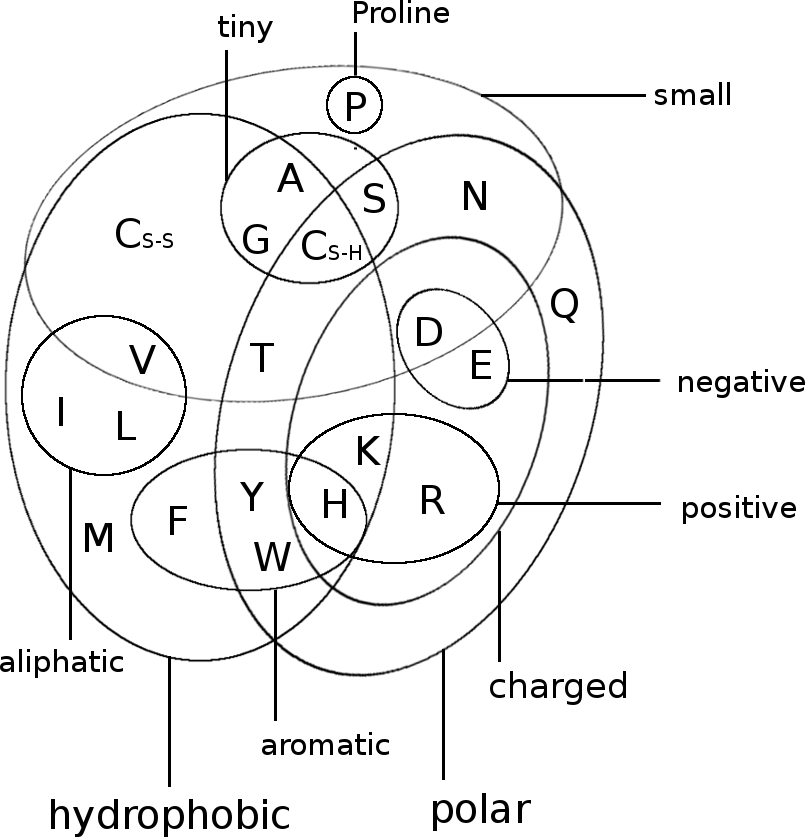
\includegraphics[width=1\linewidth]{img/amino_acid_physico_chemical_properties_venn_diagramm} \caption{Distribution of alignment diversity
(\(=\sqrt(\frac{N}{L})\)) in the dataset an its ten subsets.}\label{fig:dataset-diversity}
\end{figure}

\section{Proportion of Gaps in
Alignment}\label{proportion-of-gaps-in-alignment}




\begin{figure}
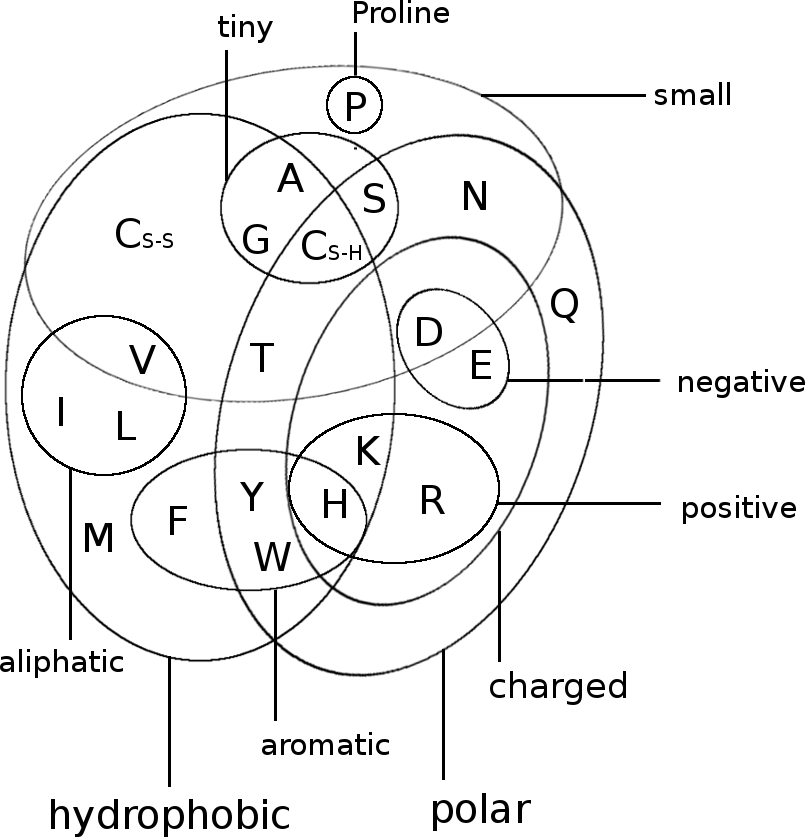
\includegraphics[width=1\linewidth]{img/amino_acid_physico_chemical_properties_venn_diagramm} \caption{Distribution of gap percentage of alignments in the
dataset an its ten subsets.}\label{fig:dataset-gaps}
\end{figure}

\section{Alignment Size (number of
sequences)}\label{alignment-size-number-of-sequences}




\begin{figure}
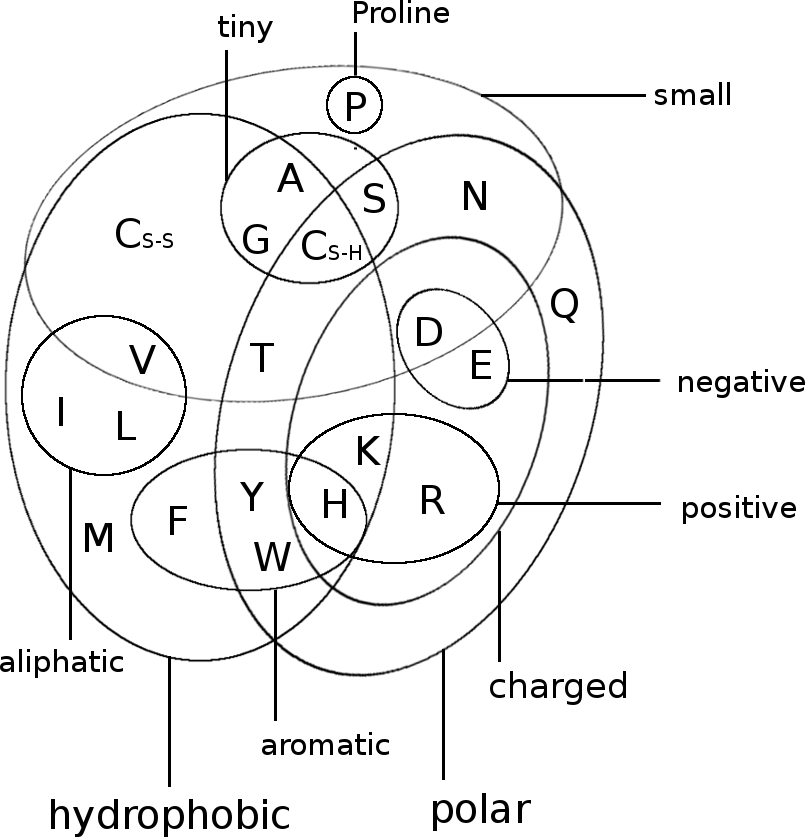
\includegraphics[width=1\linewidth]{img/amino_acid_physico_chemical_properties_venn_diagramm} \caption{Distribution of alignment size (number of
sequences N) in the dataset an its ten subsets.}\label{fig:dataset-alignment-size}
\end{figure}

\section{Protein Length}\label{protein-length}




\begin{figure}
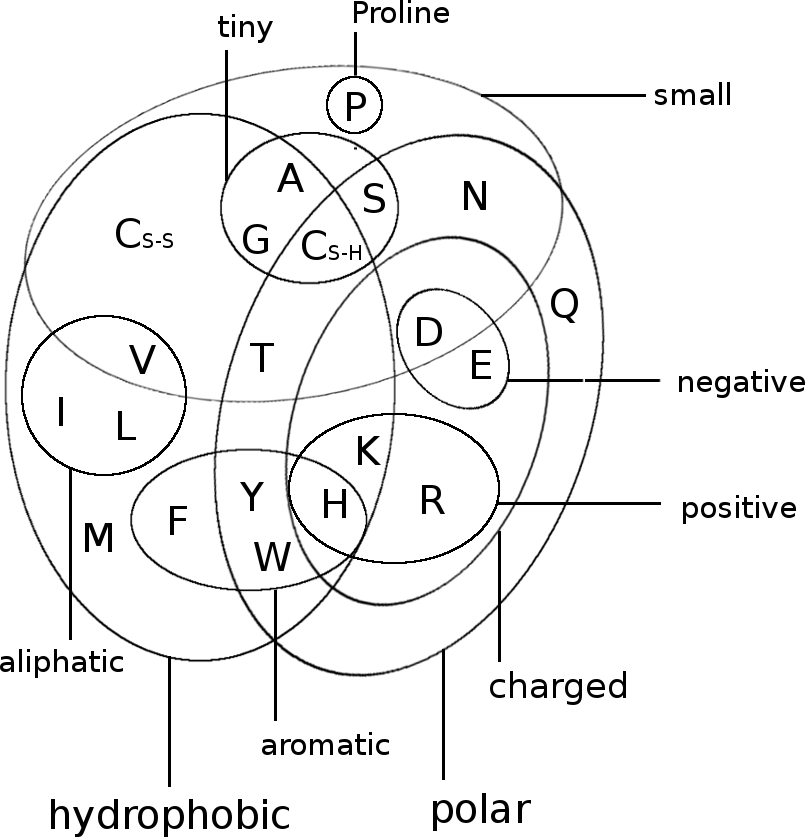
\includegraphics[width=1\linewidth]{img/amino_acid_physico_chemical_properties_venn_diagramm} \caption{Distribution of protein length L in the
dataset an its ten subsets.}\label{fig:dataset-protein-length}
\end{figure}

\chapter{Amino Acid Interaction Preferences Reflected in Coupling
Matrices}\label{amino-acid-interaction-preferences-reflected-in-coupling-matrices}

\section{Pi-Cation interactions}\label{pi-cation}

Figure \ref{fig:coupling-matrix-pication-pymol} shows a Tyrosine and a
Lysine residue forming a cation-\(\pi\) interaction in protein 2ayd. The
corresponding coupling matrix in figure
\ref{fig:coupling-matrix-pication-interaction} reflects the strong
interaction preference.





\begin{figure}
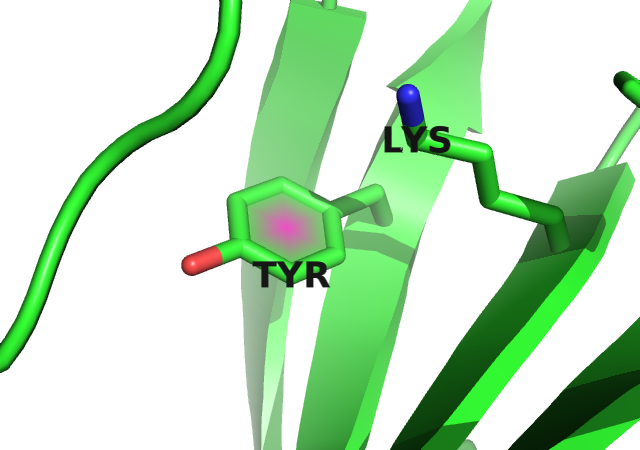
\includegraphics[width=0.5\linewidth]{img/coupling_matrix_analysis/2ayda01_37_48} \caption{Tyrosing (residue 37) and
Lysine (residue 48) forming a cation-\(\pi\) interaction in protein
2ayd.}\label{fig:coupling-matrix-pication-pymol}
\end{figure}










\begin{figure}
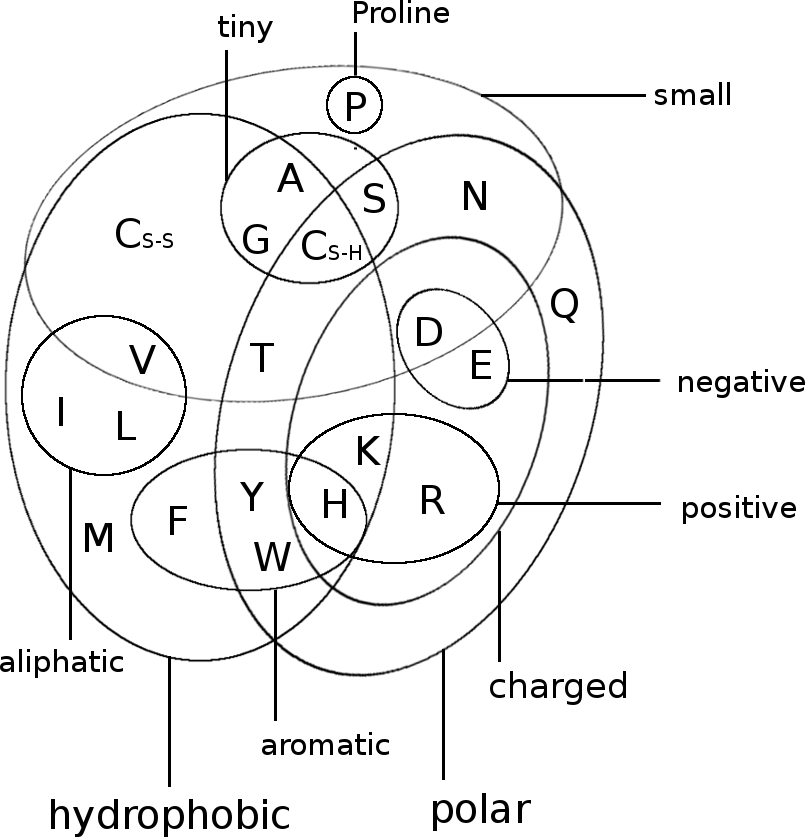
\includegraphics[width=1\linewidth]{img/amino_acid_physico_chemical_properties_venn_diagramm} \caption{Coupling Matrix for
residue pair i=37 and j=48 of PDB 2ayd chain A domain 1. Size of the
bubbles represents coupling strength and color represents the direction
of coupling: red = positive coupling, blue = negative coupling. Bars at
the x-axis represent single potentials for residue i=37 and bars at the
y-axis represent single potentials for residue j=48. Height of the bars
represents potential strength and color represents positive (red) and
negative (blue) values.}\label{fig:coupling-matrix-pication-interaction}
\end{figure}

\section{Disulfide Bonds}\label{disulfide}

Figure \ref{fig:coupling-matrix-disulfide-pymol} shows two cysteine
residues forming a covalent disulfide bond in protein 1alu. The
corresponding coupling matrix in figure
\ref{fig:coupling-matrix-disulfide-interaction} reflects the strong
interaction preference of cysteines.




\begin{figure}
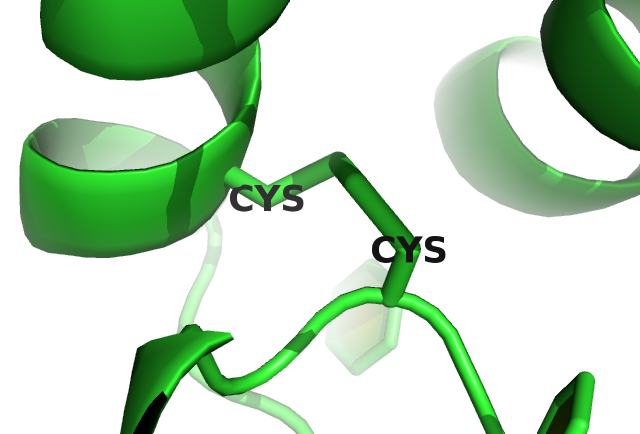
\includegraphics[width=0.5\linewidth]{img/coupling_matrix_analysis/1aluA00_54_64} \caption{Two cystein residues
(residues 54 and 64) forming a covalent disulfide bond in protein 1alu.}\label{fig:coupling-matrix-disulfide-pymol}
\end{figure}










\begin{figure}
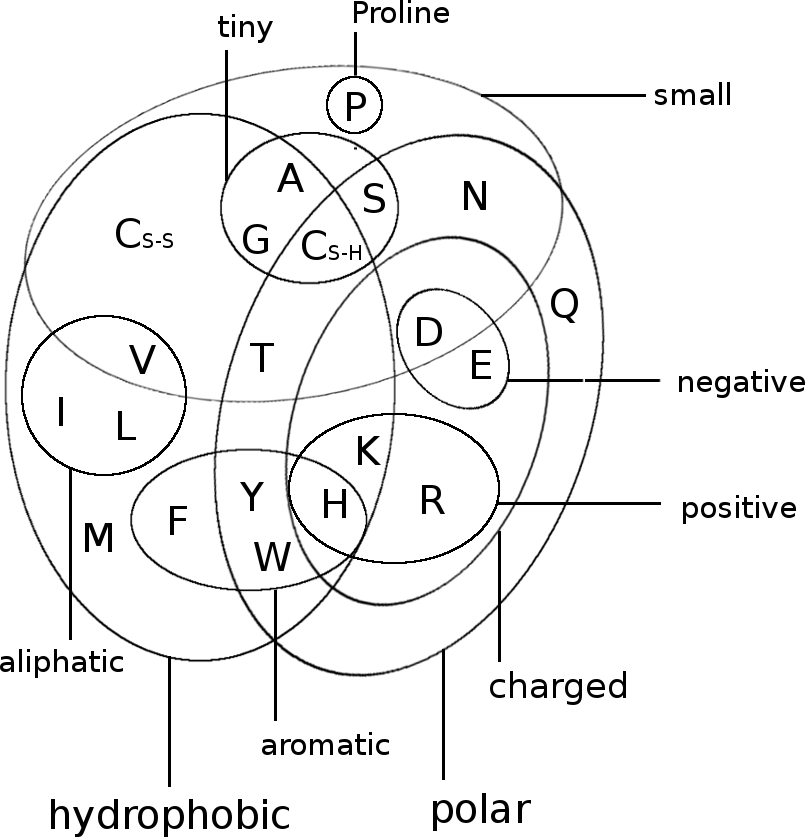
\includegraphics[width=1\linewidth]{img/amino_acid_physico_chemical_properties_venn_diagramm} \caption{Coupling Matrix for
residue pair i=54 and j=64 of PDB 1alu chain A. Size of the bubbles
represents coupling strength and color represents the direction of
coupling: red = positive coupling, blue = negative coupling. Bars at the
x-axis represent single potentials for residue i=54 and bars at the
y-axis represent single potentials for residue j=64. Height of the bars
represents potential strength and color represents positive (red) and
negative (blue) values.}\label{fig:coupling-matrix-disulfide-interaction}
\end{figure}

\section{Aromatic-Proline Interactions}\label{aromatic-proline}

Figure @ref(fig:coupling-matrix-aromatic-proline-pymol )shows a proline
and a tryptophan residue forming such a CH/\(\pi\) interaction in
protein 1aol. The corresponding coupling matrix in figure
\ref{fig:coupling-matrix-aromatic-proline} reflects this interaction
with strong positive coupling between proline and tryptophan.





\begin{figure}
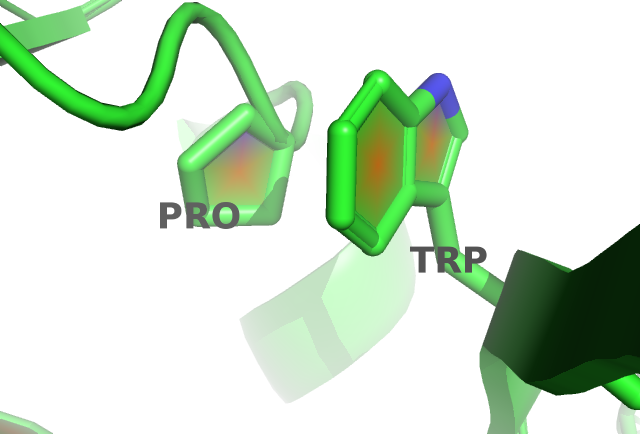
\includegraphics[width=0.5\linewidth]{img/coupling_matrix_analysis/1aolA00_17_34} \caption{Proline and
tryptophan (residues 17 and 34) stacked on top of each otherengaging in
a CH/\(\pi\) interaction in protein 1alu.}\label{fig:coupling-matrix-aromatic-proline-pymol}
\end{figure}










\begin{figure}
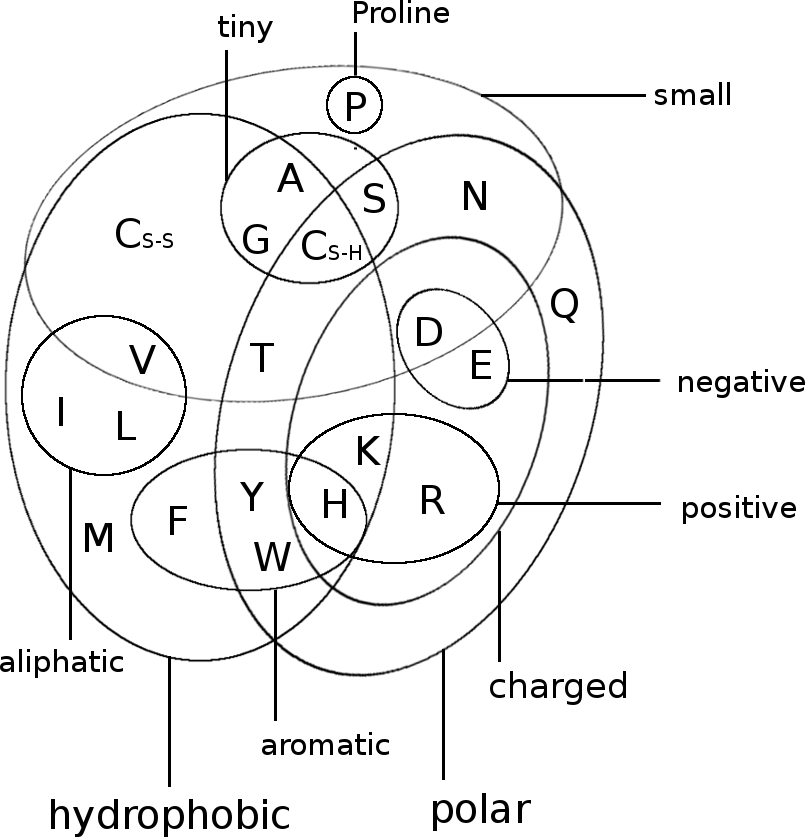
\includegraphics[width=1\linewidth]{img/amino_acid_physico_chemical_properties_venn_diagramm} \caption{Coupling Matrix for
residue pair i=17 and j=34 of PDB 1aol chain A. Size of the bubbles
represents coupling strength and color represents the direction of
coupling: red = positive coupling, blue = negative coupling. Bars at the
x-axis represent single potentials for residue i=17 and bars at the
y-axis represent single potentials for residue j=34. Height of the bars
represents potential strength and color represents positive (red) and
negative (blue) values.}\label{fig:coupling-matrix-aromatic-proline}
\end{figure}

\section{Network-like structure of aromatic
residues}\label{aromatic-network}






\begin{figure}
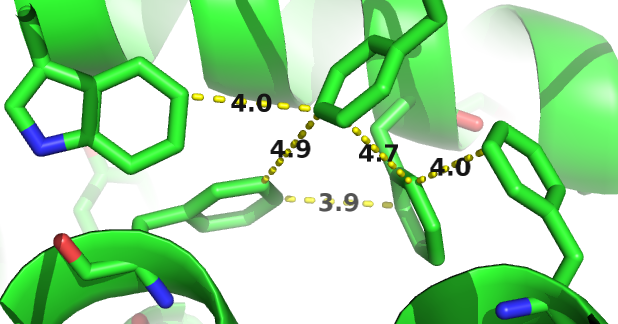
\includegraphics[width=0.5\linewidth]{img/coupling_matrix_analysis/aromatic_bundle} \caption{Network-like structure of aromatic
residues in the protein core. 80\% of aromatic residues are involved in
such networks that are important for protein stability
{[}\protect\hyperlink{ref-Burley1985}{2}{]}.}\label{fig:aromatic-network}
\end{figure}

\chapter{Optimizing Full Likelihood with Gradient
Descent}\label{optimizing-full-likelihood-with-gradient-descent}

\section{Visualisation of learning rate
schedules}\label{visualisation-of-learning-rate-schedules}















\begin{figure}

{\centering 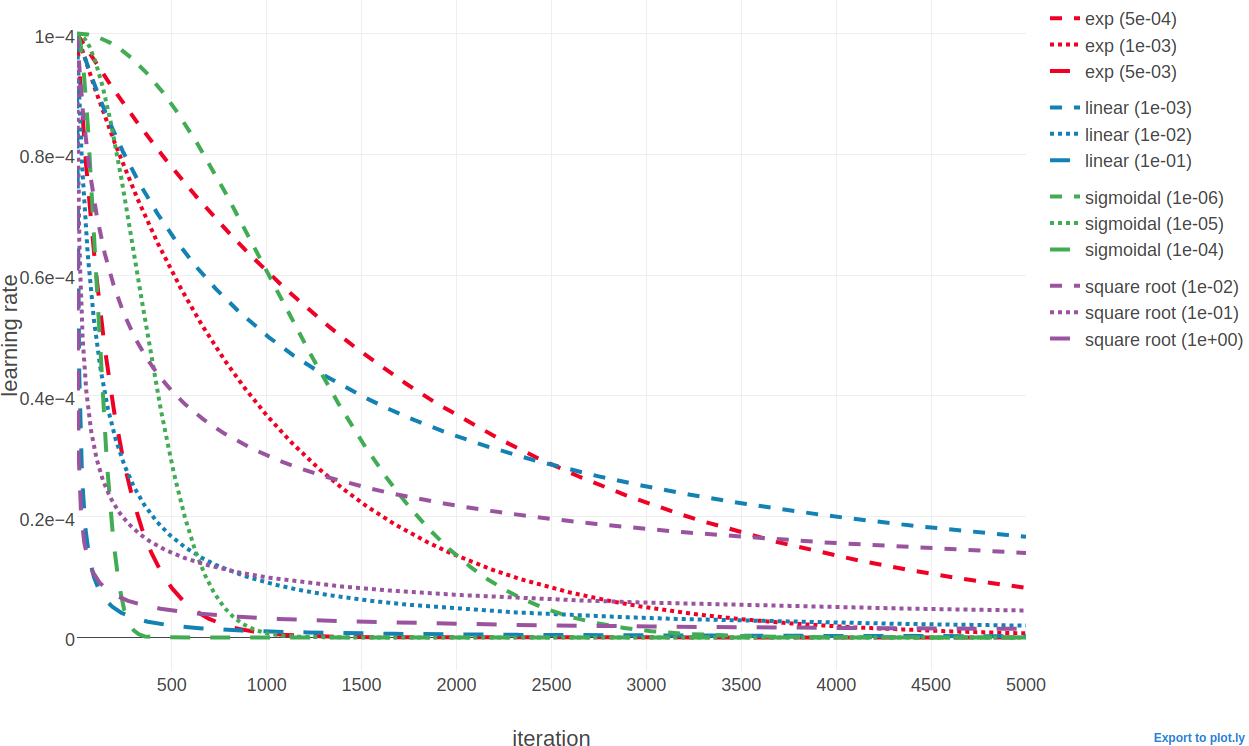
\includegraphics[width=1\linewidth]{img/full_likelihood/appendix/learning_rate_schedules_alpha0_1e-4_notitle} 

}

\caption{Value of learning rate against the
number of iterations for different learning rate schedules. Red legend
group represents the \textbf{exponential} learning rate schedule
\(\alpha_{t+1} = \alpha_0 \cdot\exp(- \gamma t)\). Blue legend group
represents the \textbf{linear} learning rate schedule
\(\alpha = \alpha_0 / (1 + \gamma \cdot t)\). Green legend group
represents the \textbf{sigmoidal} learning rate schedule
\(\alpha_{t+1} = \alpha_{t} / (1 + \gamma \cdot t)\) with \(\gamma\).
Purple legend group represents the \textbf{square root} learning rate
schedule \(\alpha = \alpha_0 / \sqrt{1 + \gamma \cdot t}\). The
iteration number is given by \(t\). Initial learning rate \(\alpha_0\)
is set to 1e-4 and \(\gamma\) is the decay rate and its value is given
in brackets in the legend.}\label{fig:learning-rate-schedules}
\end{figure}

\section{Benchmarking learning rate
schedules}\label{benchmark-learning-rate-annealing-schedules}

\subsection{Linear learning rate
schedule}\label{linear-learning-rate-schedule}












\begin{figure}

{\centering \includegraphics[width=1\linewidth]{img/full_likelihood/appendix/precision_vs_rank_alpha0_0_linear_learninrate_schedule} 

}

\caption{Mean precision for top ranked
contact predictions over 288 proteins. Contact scores are computed as
the \protect\hyperlink{abbrev}{APC} corrected Frobenius norm of the
couplings \(\wij\). pseudo-likelihood: Contact scores computed from
pseudo-likelihood. The other methods derive contact scores from
couplings computed from \protect\hyperlink{abbrev}{CD} using stochastic
gradient descent with an initial learning rate defined with respect tp
\protect\hyperlink{abbrev}{Neff} and a \emph{linear} learning rate
annealing schedule \(\alpha = \frac{\alpha_0}{1 + \gamma t}\) with decay
rate \(\gamma\) as specified in the legend.}\label{fig:performance-cd-linschedule}
\end{figure}

\subsection{Sigmoidal learning rate
schedule}\label{sigmoidal-learning-rate-schedule}













\begin{figure}

{\centering \includegraphics[width=1\linewidth]{img/full_likelihood/appendix/precision_vs_rank_alpha0_0_sigmoidal_learninrate_schedule} 

}

\caption{Mean precision for top ranked
contact predictions over 288 proteins. Contact scores are computed as
the \protect\hyperlink{abbrev}{APC} corrected Frobenius norm of the
couplings \(\wij\). pseudo-likelihood: Contact scores computed from
pseudo-likelihood. The other methods derive contact scores from
couplings computed from \protect\hyperlink{abbrev}{CD} using stochastic
gradient descent with an initial learning rate defined with respect tp
\protect\hyperlink{abbrev}{Neff} and a \emph{sigmoidal} learning rate
annealing schedule \(\alpha_{t+1} = \frac{\alpha_{t}}{1 + \gamma t}\)
with t being the iteration number and decay rate \(\gamma\) as specified
in the legend.}\label{fig:performance-cd-sigschedule}
\end{figure}

\subsection{Square root learning rate
schedule}\label{square-root-learning-rate-schedule}

\subsection{Exponential learning rate
schedule}\label{exponential-learning-rate-schedule}

\section{Number of iterations until convergence for different learning
rate schedules}\label{learning-rate-schedules-distribution-iterations}

\subsection{Linear learning rate
schedule}\label{linear-learning-rate-schedule-1}

(ref:caption-full-likelihood-opt-numit\_lin\_learning-rate-schedule)
Distribution of the number of iterations until convergence for gradient
descent optimizations of the full likelihood using different decay rates
with a \emph{linear} learning rate schedule
\(\alpha = \alpha_0 / (1 + \gamma \cdot t)\) with t being the iteration
number and the decay rate \(\gamma\) as specified in the legend. Initial
learning rate \(\alpha_0\) defined with respect tp
\protect\hyperlink{abbrev}{Neff} and maximum number of iterations is set
to 5000.

\begin{figure}

{\centering \includegraphics[width=0.9\linewidth]{img/full_likelihood/appendix/distribution_numiterations_against_linear_learningrate_schedule} 

}

\caption{(ref:caption-full-likelihood-opt-numit-lin-learning-rate-schedule)}\label{fig:full-likelihood-opt-numit-lin-learning-rate-schedule}
\end{figure}

\subsection{Sigmoidal learning rate
schedule}\label{sigmoidal-learning-rate-schedule-1}

(ref:caption-numit\_convergence-sig\_learning-rate-schedule)
Distribution of the number of iterations until convergence for gradient
descent optimizations of the full likelihood using different decay rates
with a \emph{sigmoidal} learning rate schedule
\(\alpha_{t+1} = \alpha_{t} / (1 + \gamma \cdot t)\) with t being the
iteration number and the decay rate \(\gamma\) as specified in the
legend. Initial learning rate \(\alpha_0\) defined with respect tp
\protect\hyperlink{abbrev}{Neff} and maximum number of iterations is set
to 5000.

\begin{figure}

{\centering \includegraphics[width=1\linewidth]{img/full_likelihood/appendix/distribution_numiterations_against_sigmoidal_learningrate_schedule} 

}

\caption{(ref:caption-numit_convergence-sig_learning-rate-schedule)}(\#fig:numit_convergence-sig_learning-rate-schedule)
\end{figure}

\subsection{Square root learning rate
schedule}\label{square-root-learning-rate-schedule-1}

(ref:caption-full-likelihood-opt-numit\_sqrt\_learning-rate-schedule)
Distribution of the number of iterations until convergence for gradient
descent optimizations of the full likelihood using different decay rates
with a square root learning rate schedule. Initial learning rate
\(\alpha_0\) is fixed to 1e-4 and maximum number of iterations is set to
5000. The learning rate is decreased according to
\(\alpha_{t+1} = \alpha_{t} / (1 + \gamma \cdot t)\) with t being the
iteration number and \(\gamma\) the decay rate and its value is given
after the underscore in the legend names.

\begin{figure}

{\centering \includegraphics[width=0.9\linewidth]{img/full_likelihood/appendix/distribution_numiterations_against_alpha1e-4_sqrtdecay} 

}

\caption{(ref:caption-full-likelihood-opt-numit-sqrt-learning-rate-schedule)}\label{fig:full-likelihood-opt-numit-sqrt-learning-rate-schedule}
\end{figure}

\subsection{Exponential learning rate
schedule}\label{exponential-learning-rate-schedule-1}

\chapter{Training of the Random Forest Contact
Prior}\label{training-of-the-random-forest-contact-prior}

\section{Evaluating window size with 5-fold
Cross-validation}\label{rf-window-size}








\begin{figure}

{\centering \includegraphics[width=0.9\linewidth]{img/random_forest_contact_prior/cross_validation/precision_vs_rank_cv_on_test_random_forest_nestimators1000_maxfeatureslog2_maxdepth10_minsamplesleaf100_windowsize} 

}

\caption{Mean precision over
validation set of 200 proteins for top ranked contact predictions for
different choices of window size for single position features. Dashed
lines represent the models trained on four subsets of the training data
according to the 5-fold cross-validation scheme. Solid lines represent
the mean over the five cross-validation models.}\label{fig:random-forest-window-size-cv}
\end{figure}

\section{Evaluating non-contact threshold with 5-fold
Cross-validation}\label{rf-noncontact-threshold}








\begin{figure}

{\centering \includegraphics[width=0.9\linewidth]{img/random_forest_contact_prior/cross_validation/precision_vs_rank_cv_on_test_random_forest_nestimators1000_maxfeatureslog2_maxdepth10_minsamplesleaf100_noncontactthr} 

}

\caption{Mean precision over
validation set of 200 proteins for top ranked contact predictions for
different choices of the non-contact threshold to define non-contacts.
Dashed lines represent the models trained on four subsets of the
training data according to the 5-fold cross-validation scheme. Solid
lines represent the mean over the five cross-validation models.}\label{fig:random-forest-noncontactthr-cv}
\end{figure}

\section{Evaluating ratio of non-contacts and contacts in the training
set with 5-fold Cross-validation}\label{rf-ratio-noncontacts}









\begin{figure}

{\centering \includegraphics[width=0.9\linewidth]{img/random_forest_contact_prior/cross_validation/precision_vs_rank_cv_on_test_random_forest_nestimators1000_maxfeatureslog2_maxdepth10_minsamplesleaf100_ratio} 

}

\caption{Mean precision over
validation set of 200 proteins for top ranked contact predictions for
different choices of dataset composition with respect to the ratio of
contacts and non-contacts. Dashed lines represent the models trained on
four subsets of the training data according to the 5-fold
cross-validation scheme. Solid lines represent the mean over the five
cross-validation models.}\label{fig:random-forest-rationoncontactthr-cv}
\end{figure}

\backmatter

\listoffigures
\addcontentsline{toc}{chapter}{List of Figures}

\listoftables
\addcontentsline{toc}{chapter}{List of Tables}

\chapter*{References}\label{references}
\addcontentsline{toc}{chapter}{References}

\hypertarget{refs}{}
\hypertarget{ref-Coucke2016}{}
1. Coucke, A., Uguzzoni, G., Oteri, F., Cocco, S., Monasson, R., and
Weigt, M. (2016). Direct coevolutionary couplings reflect biophysical
residue interactions in proteins. J. Chem. Phys. \emph{145}, 174102.
Available at:
\url{http://scitation.aip.org/content/aip/journal/jcp/145/17/10.1063/1.4966156}.

\hypertarget{ref-Burley1985}{}
2. Burley, S., and Petsko, G. (1985). Aromatic-aromatic interaction: a
mechanism of protein structure stabilization. Science (80-. ).
\emph{229}, 23--28. Available at:
\url{http://www.sciencemag.org/cgi/doi/10.1126/science.3892686}.

\hypertarget{ref-Jones2015a}{}
3. Jones, D.T., Singh, T., Kosciolek, T., and Tetchner, S. (2015).
MetaPSICOV: combining coevolution methods for accurate prediction of
contacts and long range hydrogen bonding in proteins. Bioinformatics
\emph{31}, 999--1006. Available at:
\url{http://bioinformatics.oxfordjournals.org/content/31/7/999.short}.

\hypertarget{ref-He2017}{}
4. He, B., Mortuza, S.M., Wang, Y., Shen, H.-B., and Zhang, Y. (2017).
NeBcon: Protein contact map prediction using neural network training
coupled with naïve Bayes classifiers. Bioinformatics. Available at:
\url{https://academic.oup.com/bioinformatics/article-lookup/doi/10.1093/bioinformatics/btx164}.

\hypertarget{ref-Stahl2017}{}
5. Stahl, K., Schneider, M., and Brock, O. (2017). EPSILON-CP: using
deep learning to combine information from multiple sources for protein
contact prediction. BMC Bioinformatics \emph{18}, 303. Available at:
\url{http://bmcbioinformatics.biomedcentral.com/articles/10.1186/s12859-017-1713-x}.

\hypertarget{ref-Skwark2016}{}
6. Skwark, M.J., Michel, M., Menendez Hurtado, D., Ekeberg, M., and
Elofsson, A. (2016). Accurate contact predictions for thousands of
protein families using PconsC3. bioRxiv.

\hypertarget{ref-Ma2015a}{}
7. Ma, J., Wang, S., Wang, Z., and Xu, J. (2015). Protein contact
prediction by integrating joint evolutionary coupling analysis and
supervised learning. Bioinformatics, btv472. Available at:
\url{http://bioinformatics.oxfordjournals.org/content/early/2015/09/04/bioinformatics.btv472}.

\hypertarget{ref-Ho1998}{}
8. Ho, T.K. (1998). The random subspace method for constructing decision
forests. IEEE Trans. Pattern Anal. Mach. Intell. \emph{20}, 832--844.
Available at: \url{http://ieeexplore.ieee.org/document/709601/}.

\hypertarget{ref-TinKamHo}{}
9. Tin Kam Ho (1995). Random decision forests. In Proc. 3rd int. conf.
doc. anal. recognit. (IEEE Comput. Soc. Press), pp. 278--282. Available
at: \url{http://ieeexplore.ieee.org/document/598994/}.

\hypertarget{ref-Breiman2001}{}
10. Breiman, L. (2001). Random Forests. Mach. Learn. \emph{45}, 5--32.
Available at: \url{http://link.springer.com/10.1023/A:1010933404324}.

\hypertarget{ref-Menze2009}{}
11. Menze, B.H., Kelm, B.M., Masuch, R., Himmelreich, U., Bachert, P.,
Petrich, W., and Hamprecht, F.A. (2009). A comparison of random forest
and its Gini importance with standard chemometric methods for the
feature selection and classification of spectral data. BMC
Bioinformatics \emph{10}, 213. Available at:
\href{http://www.ncbi.nlm.nih.gov/pubmed/19591666\%20http://www.pubmedcentral.nih.gov/articlerender.fcgi?artid=PMC2724423}{http://www.ncbi.nlm.nih.gov/pubmed/19591666 http://www.pubmedcentral.nih.gov/articlerender.fcgi?artid=PMC2724423}.

\hypertarget{ref-Louppe2014}{}
12. Louppe, G. (2014). Understanding Random Forests: From Theory to
Practice. Available at: \url{http://arxiv.org/abs/1407.7502}.

\hypertarget{ref-Strobl2007}{}
13. Strobl, C., Boulesteix, A.-L., Zeileis, A., and Hothorn, T. (2007).
Bias in random forest variable importance measures: Illustrations,
sources and a solution. BMC Bioinformatics \emph{8}, 25. Available at:
\url{http://bmcbioinformatics.biomedcentral.com/articles/10.1186/1471-2105-8-25}.

\hypertarget{ref-Fodor2004a}{}
14. Fodor, A.A., and Aldrich, R.W. (2004). Influence of conservation on
calculations of amino acid covariance in multiple sequence alignments.
Proteins \emph{56}, 211--21. Available at:
\url{http://www.ncbi.nlm.nih.gov/pubmed/15211506}.

\hypertarget{ref-Miyazawa1999a}{}
15. Miyazawa, S., and Jernigan, R.L. (1999). Self-consistent estimation
of inter-residue protein contact energies based on an equilibrium
mixture approximation of residues. Proteins \emph{34}, 49--68. Available
at: \url{http://www.ncbi.nlm.nih.gov/pubmed/10336383}.

\hypertarget{ref-Li2011}{}
16. Li, Y., Fang, Y., and Fang, J. (2011). Predicting residue-residue
contacts using random forest models. Bioinformatics \emph{27}, 3379--84.
Available at:
\url{http://bioinformatics.oxfordjournals.org/content/27/24/3379.long}.

\hypertarget{ref-Petersen2009a}{}
17. Petersen, B., Petersen, T.N., Andersen, P., Nielsen, M., and
Lundegaard, C. (2009). BMC Structural Biology A generic method for
assignment of reliability scores applied to solvent accessibility
predictions. BMC Struct. Biol. \emph{9}. Available at:
\url{http://www.biomedcentral.com/1472-6807/9/51}.

\hypertarget{ref-Jones1999}{}
18. Jones, D.T. (1999). Protein secondary structure prediction based on
position-specific scoring matrices 1 1Edited by G. Von Heijne. J. Mol.
Biol. \emph{292}, 195--202. Available at:
\href{http://www.ncbi.nlm.nih.gov/pubmed/10493868\%20http://linkinghub.elsevier.com/retrieve/pii/S0022283699930917}{http://www.ncbi.nlm.nih.gov/pubmed/10493868 http://linkinghub.elsevier.com/retrieve/pii/S0022283699930917}.

\hypertarget{ref-Sillitoe2015}{}
19. Sillitoe, I., Lewis, T.E., Cuff, A., Das, S., Ashford, P., Dawson,
N.L., Furnham, N., Laskowski, R.A., Lee, D., and Lees, J.G. \emph{et
al.} (2015). CATH: comprehensive structural and functional annotations
for genome sequences. Nucleic Acids Res. \emph{43}, D376--D381.
Available at:
\url{https://academic.oup.com/nar/article-lookup/doi/10.1093/nar/gku947}.

\hypertarget{ref-Remmert2012}{}
20. Remmert, M., Biegert, A., Hauser, A., and Söding, J. (2012).
HHblits: lightning-fast iterative protein sequence searching by HMM-HMM
alignment. Nat. Methods \emph{9}, 173--5. Available at:
\url{http://dx.doi.org/10.1038/nmeth.1818}.

\hypertarget{ref-Seemayer2014}{}
21. Seemayer, S., Gruber, M., and Söding, J. (2014). CCMpred-fast and
precise prediction of protein residue-residue contacts from correlated
mutations. Bioinformatics, btu500. Available at:
\url{http://bioinformatics.oxfordjournals.org/content/early/2014/08/12/bioinformatics.btu500}.

\hypertarget{ref-Stein2015a}{}
22. Stein, R.R., Marks, D.S., and Sander, C. (2015). Inferring Pairwise
Interactions from Biological Data Using Maximum-Entropy Probability
Models. PLOS Comput. Biol. \emph{11}, e1004182. Available at:
\href{http://www.pubmedcentral.nih.gov/articlerender.fcgi?artid=4520494\%7B/\&\%7Dtool=pmcentrez\%7B/\&\%7Drendertype=abstract}{http://www.pubmedcentral.nih.gov/articlerender.fcgi?artid=4520494\{\textbackslash{}\&\}tool=pmcentrez\{\textbackslash{}\&\}rendertype=abstract}.

\hypertarget{ref-Buslje2009}{}
23. Buslje, C.M., Santos, J., Delfino, J.M., and Nielsen, M. (2009).
Correction for phylogeny, small number of observations and data
redundancy improves the identification of coevolving amino acid pairs
using mutual information. Bioinformatics \emph{25}, 1125--31. Available
at:
\href{http://www.ncbi.nlm.nih.gov/pubmed/19276150\%20http://www.pubmedcentral.nih.gov/articlerender.fcgi?artid=PMC2672635}{http://www.ncbi.nlm.nih.gov/pubmed/19276150 http://www.pubmedcentral.nih.gov/articlerender.fcgi?artid=PMC2672635}.

\hypertarget{ref-Morcos2011}{}
24. Morcos, F., Pagnani, A., Lunt, B., Bertolino, A., Marks, D.S.,
Sander, C., Zecchina, R., Onuchic, J.N., Hwa, T., and Weigt, M. (2011).
Direct-coupling analysis of residue coevolution captures native contacts
across many protein families. Proc. Natl. Acad. Sci. U. S. A.
\emph{108}, E1293--301. Available at:
\url{http://www.pnas.org/content/108/49/E1293.full}.

\hypertarget{ref-Jones2012}{}
25. Jones, D.T., Buchan, D.W.A., Cozzetto, D., and Pontil, M. (2012).
PSICOV: precise structural contact prediction using sparse inverse
covariance estimation on large multiple sequence alignments.
Bioinformatics \emph{28}, 184--90. Available at:
\url{http://bioinformatics.oxfordjournals.org/content/28/2/184.full}.

\hypertarget{ref-Carreira-Perpinan2005}{}
26. Carreira-Perpiñán, M. a, and Hinton, G.E. (2005). On Contrastive
Divergence Learning. Artif. Intell. Stat. \emph{0}, 17. Available at:
\href{http://learning.cs.toronto.edu/\%7B~\%7Dhinton/absps/cdmiguel.pdf}{http://learning.cs.toronto.edu/\{\textasciitilde{}\}hinton/absps/cdmiguel.pdf}.

\hypertarget{ref-Le2011}{}
27. Le, Q.V., Ngiam, J., Coates, A., Lahiri, A., Prochnow, B., and Ng,
A.Y. (2011). On optimization methods for deep learning ({[}International
Machine Learning Society{]}) Available at:
\url{https://dl.acm.org/citation.cfm?id=3104516}.

\hypertarget{ref-Kingma2014}{}
28. Kingma, D., and Ba, J. (2014). Adam: A Method for Stochastic
Optimization. Available at: \url{http://arxiv.org/abs/1412.6980}.

\hypertarget{ref-Chollet2015}{}
29. Chollet, F. and others (2015). Keras. Available at:
\url{https://github.com/fchollet/keras}.

\hypertarget{ref-Dieleman2015}{}
30. Dieleman, S., Schlüter, J., Raffel, C., Olson, E., Sønderby, S.K.,
Nouri, D., Maturana, D., Thoma, M., Battenberg, E., and Kelly, J.
\emph{et al.} (2015). Lasagne: First release. Available at:
\url{https://zenodo.org/record/27878}.

\hypertarget{ref-Bottou2012}{}
31. Bottou, L. (2012). Stochastic Gradient Descent Tricks. In Neural
networks: Tricks of the trade (Springer, Berlin, Heidelberg), pp.
421--436. Available at:
\href{http://link.springer.com/10.1007/978-3-642-35289-8\%7B/_\%7D25}{http://link.springer.com/10.1007/978-3-642-35289-8\{\textbackslash{}\_\}25}.

\hypertarget{ref-Hinton2002}{}
32. Hinton, G.E. (2002). Training Products of Experts by Minimizing
Contrastive Divergence. Neural Comput. \emph{14}, 1771--1800. Available
at: \url{http://www.gatsby.ucl.ac.uk/publications/tr/tr00-004.pdf}.

\hypertarget{ref-Bengio2009}{}
33. Bengio, Y., and Delalleau, O. (2009). Justifying and Generalizing
Contrastive Divergence. Neural Comput. \emph{21}, 1601--21. Available
at:
\href{http://www.iro.umontreal.ca/\%7B~\%7Dlisa/publications2/index.php/attachments/single/105}{http://www.iro.umontreal.ca/\{\textasciitilde{}\}lisa/publications2/index.php/attachments/single/105}.

\hypertarget{ref-Tieleman2008}{}
34. Tieleman, T. (2008). Training Restricted Boltzmann Machines using
Approximations to the Likelihood Gradient. Proc. 25th Int. Conf. Mach.
Learn. \emph{307}, 7.

\hypertarget{ref-Robinson1991}{}
35. Robinson, A.B., and Robinson, L.R. (1991). Distribution of glutamine
and asparagine residues and their near neighbors in peptides and
proteins. Proc. Natl. Acad. Sci. U. S. A. \emph{88}, 8880--4. Available
at:
\href{http://www.ncbi.nlm.nih.gov/pubmed/1924347\%20http://www.pubmedcentral.nih.gov/articlerender.fcgi?artid=PMC52614}{http://www.ncbi.nlm.nih.gov/pubmed/1924347 http://www.pubmedcentral.nih.gov/articlerender.fcgi?artid=PMC52614}.

\hypertarget{ref-Atchley2005}{}
36. Atchley, W.R., Zhao, J., Fernandes, A.D., and Drüke, T. (2005).
Solving the protein sequence metric problem. Proc. Natl. Acad. Sci. U.
S. A. \emph{102}, 6395--400. Available at:
\url{http://www.pnas.org/content/102/18/6395.abstract}.

\hypertarget{ref-Kawashima2008}{}
37. Kawashima, S., Pokarowski, P., Pokarowska, M., Kolinski, A.,
Katayama, T., and Kanehisa, M. (2008). AAindex: amino acid index
database, progress report 2008. Nucleic Acids Res. \emph{36}, D202--5.
Available at:
\href{http://www.ncbi.nlm.nih.gov/pubmed/17998252\%20http://www.pubmedcentral.nih.gov/articlerender.fcgi?artid=PMC2238890}{http://www.ncbi.nlm.nih.gov/pubmed/17998252 http://www.pubmedcentral.nih.gov/articlerender.fcgi?artid=PMC2238890}.

\hypertarget{ref-Wimley1996}{}
38. Wimley, W.C., and White, S.H. (1996). Experimentally determined
hydrophobicity scale for proteins at membrane interfaces. Nat. Struct.
Biol. \emph{3}, 842--8. Available at:
\url{http://www.ncbi.nlm.nih.gov/pubmed/8836100}.

\hypertarget{ref-Cornette1987}{}
39. Cornette, J.L., Cease, K.B., Margalit, H., Spouge, J.L., Berzofsky,
J.A., and DeLisi, C. (1987). Hydrophobicity scales and computational
techniques for detecting amphipathic structures in proteins. J. Mol.
Biol. \emph{195}, 659--685. Available at:
\url{http://linkinghub.elsevier.com/retrieve/pii/0022283687901896}.

\hypertarget{ref-Zhu1999}{}
40. Zhu, H., and Braun, W. (1999). Sequence specificity, statistical
potentials, and three-dimensional structure prediction with
self-correcting distance geometry calculations of beta-sheet formation
in proteins. Protein Sci. \emph{8}, 326--42. Available at:
\href{http://www.pubmedcentral.nih.gov/articlerender.fcgi?artid=2144259\%7B/\&\%7Dtool=pmcentrez\%7B/\&\%7Drendertype=abstract}{http://www.pubmedcentral.nih.gov/articlerender.fcgi?artid=2144259\{\textbackslash{}\&\}tool=pmcentrez\{\textbackslash{}\&\}rendertype=abstract}.

\hypertarget{ref-Bernard2009}{}
41. Bernard, S., Heutte, L., and Adam, S. (2009). Influence of
Hyperparameters on Random Forest Accuracy. In (Springer, Berlin,
Heidelberg), pp. 171--180. Available at:
\href{http://link.springer.com/10.1007/978-3-642-02326-2\%7B/_\%7D18}{http://link.springer.com/10.1007/978-3-642-02326-2\{\textbackslash{}\_\}18}.

\hypertarget{ref-Pedregosa2011}{}
42. Pedregosa, F., Varoquaux, G., Gramfort, A., Michel, V., Thirion, B.,
Grisel, O., Blondel, M., Prettenhofer, P., Weiss, R., and Dubourg, V.
\emph{et al.} (2011). Scikit-learn: Machine Learning in Python. J. Mach.
Learn. Res. \emph{12}, 2825--2830. Available at:
\url{http://jmlr.csail.mit.edu/papers/v12/pedregosa11a.html}.

\hypertarget{ref-Wu2008}{}
43. Wu, S., and Zhang, Y. (2008). A comprehensive assessment of
sequence-based and template-based methods for protein contact
prediction. Bioinformatics \emph{24}, 924--31. Available at:
\href{http://www.pubmedcentral.nih.gov/articlerender.fcgi?artid=2648832\%7B/\&\%7Dtool=pmcentrez\%7B/\&\%7Drendertype=abstract}{http://www.pubmedcentral.nih.gov/articlerender.fcgi?artid=2648832\{\textbackslash{}\&\}tool=pmcentrez\{\textbackslash{}\&\}rendertype=abstract}.

\hypertarget{ref-Wang2011}{}
44. Wang, X.-F., Chen, Z., Wang, C., Yan, R.-X., Zhang, Z., and Song, J.
(2011). Predicting residue-residue contacts and helix-helix interactions
in transmembrane proteins using an integrative feature-based random
forest approach. PLoS One \emph{6}, e26767. Available at:
\href{http://www.pubmedcentral.nih.gov/articlerender.fcgi?artid=3203928\%7B/\&\%7Dtool=pmcentrez\%7B/\&\%7Drendertype=abstract}{http://www.pubmedcentral.nih.gov/articlerender.fcgi?artid=3203928\{\textbackslash{}\&\}tool=pmcentrez\{\textbackslash{}\&\}rendertype=abstract}.

\hypertarget{ref-DiLena2012a}{}
45. Di Lena, P., Nagata, K., and Baldi, P. (2012). Deep architectures
for protein contact map prediction. Bioinformatics \emph{28}, 2449--57.
Available at:
\href{http://bioinformatics.oxfordjournals.org/content/28/19/2449.full\%7B/\#\%7Dsec-14}{http://bioinformatics.oxfordjournals.org/content/28/19/2449.full\{\textbackslash{}\#\}sec-14}.

\hypertarget{ref-Wang2013}{}
46. Wang, Z., and Xu, J. (2013). Predicting protein contact map using
evolutionary and physical constraints by integer programming.
Bioinformatics \emph{29}, i266--73. Available at:
\href{http://www.pubmedcentral.nih.gov/articlerender.fcgi?artid=3694661\%7B/\&\%7Dtool=pmcentrez\%7B/\&\%7Drendertype=abstract}{http://www.pubmedcentral.nih.gov/articlerender.fcgi?artid=3694661\{\textbackslash{}\&\}tool=pmcentrez\{\textbackslash{}\&\}rendertype=abstract}.

\hypertarget{ref-Cheng2007}{}
47. Cheng, J., and Baldi, P. (2007). Improved residue contact prediction
using support vector machines and a large feature set. BMC
Bioinformatics \emph{8}, 113. Available at:
\href{http://www.pubmedcentral.nih.gov/articlerender.fcgi?artid=1852326\%7B/\&\%7Dtool=pmcentrez\%7B/\&\%7Drendertype=abstract}{http://www.pubmedcentral.nih.gov/articlerender.fcgi?artid=1852326\{\textbackslash{}\&\}tool=pmcentrez\{\textbackslash{}\&\}rendertype=abstract}.


\end{document}
